\documentclass[10pt]{article}

\usepackage{fullpage,amsmath,amssymb,amsfonts,booktabs,float,graphicx,longtable,parskip}
\usepackage[colorlinks=true, linkcolor=black]{hyperref}

\usepackage{pdfpages,graphics}
\usepackage{booktabs}
\usepackage{multicol,fullpage}
\usepackage[margin=0.7in]{geometry}
\usepackage[utf8x]{inputenc}
\usepackage[T1]{fontenc}
\usepackage{textcomp}
\usepackage{textgreek}
\usepackage{bm}

\usepackage{afterpage,adjustbox}
\usepackage{url}

\usepackage{microtype}

\usepackage{enumitem}
\setlist[enumerate]{leftmargin=*, topsep=0pt,itemsep=2pt,partopsep=0pt,parsep=0pt}
\setitemize{leftmargin=*, noitemsep,topsep=0pt,parsep=2pt,partopsep=0pt}

\setlength{\parindent}{0em}
\setlength{\parskip}{0.5em}
\setlength{\columnsep}{2em}
\setlength{\columnseprule}{0.2pt}

\renewcommand{\UrlBreaks}{\do\/\do\a\do\b\do\c\do\d\do\e\do\f\do\g\do\h\do\i\do\j\do\k\do\l\do\m\do\n\do\o\do\p\do\q\do\r\do\s\do\t\do\u\do\v\do\w\do\x\do\y\do\z\do\A\do\B\do\C\do\D\do\E\do\F\do\G\do\H\do\I\do\J\do\K\do\L\do\M\do\N\do\O\do\P\do\Q\do\R\do\S\do\T\do\U\do\V\do\W\do\X\do\Y\do\Z}

\begin{document}

\hspace{0pt}
\vfill

\begin{center}
  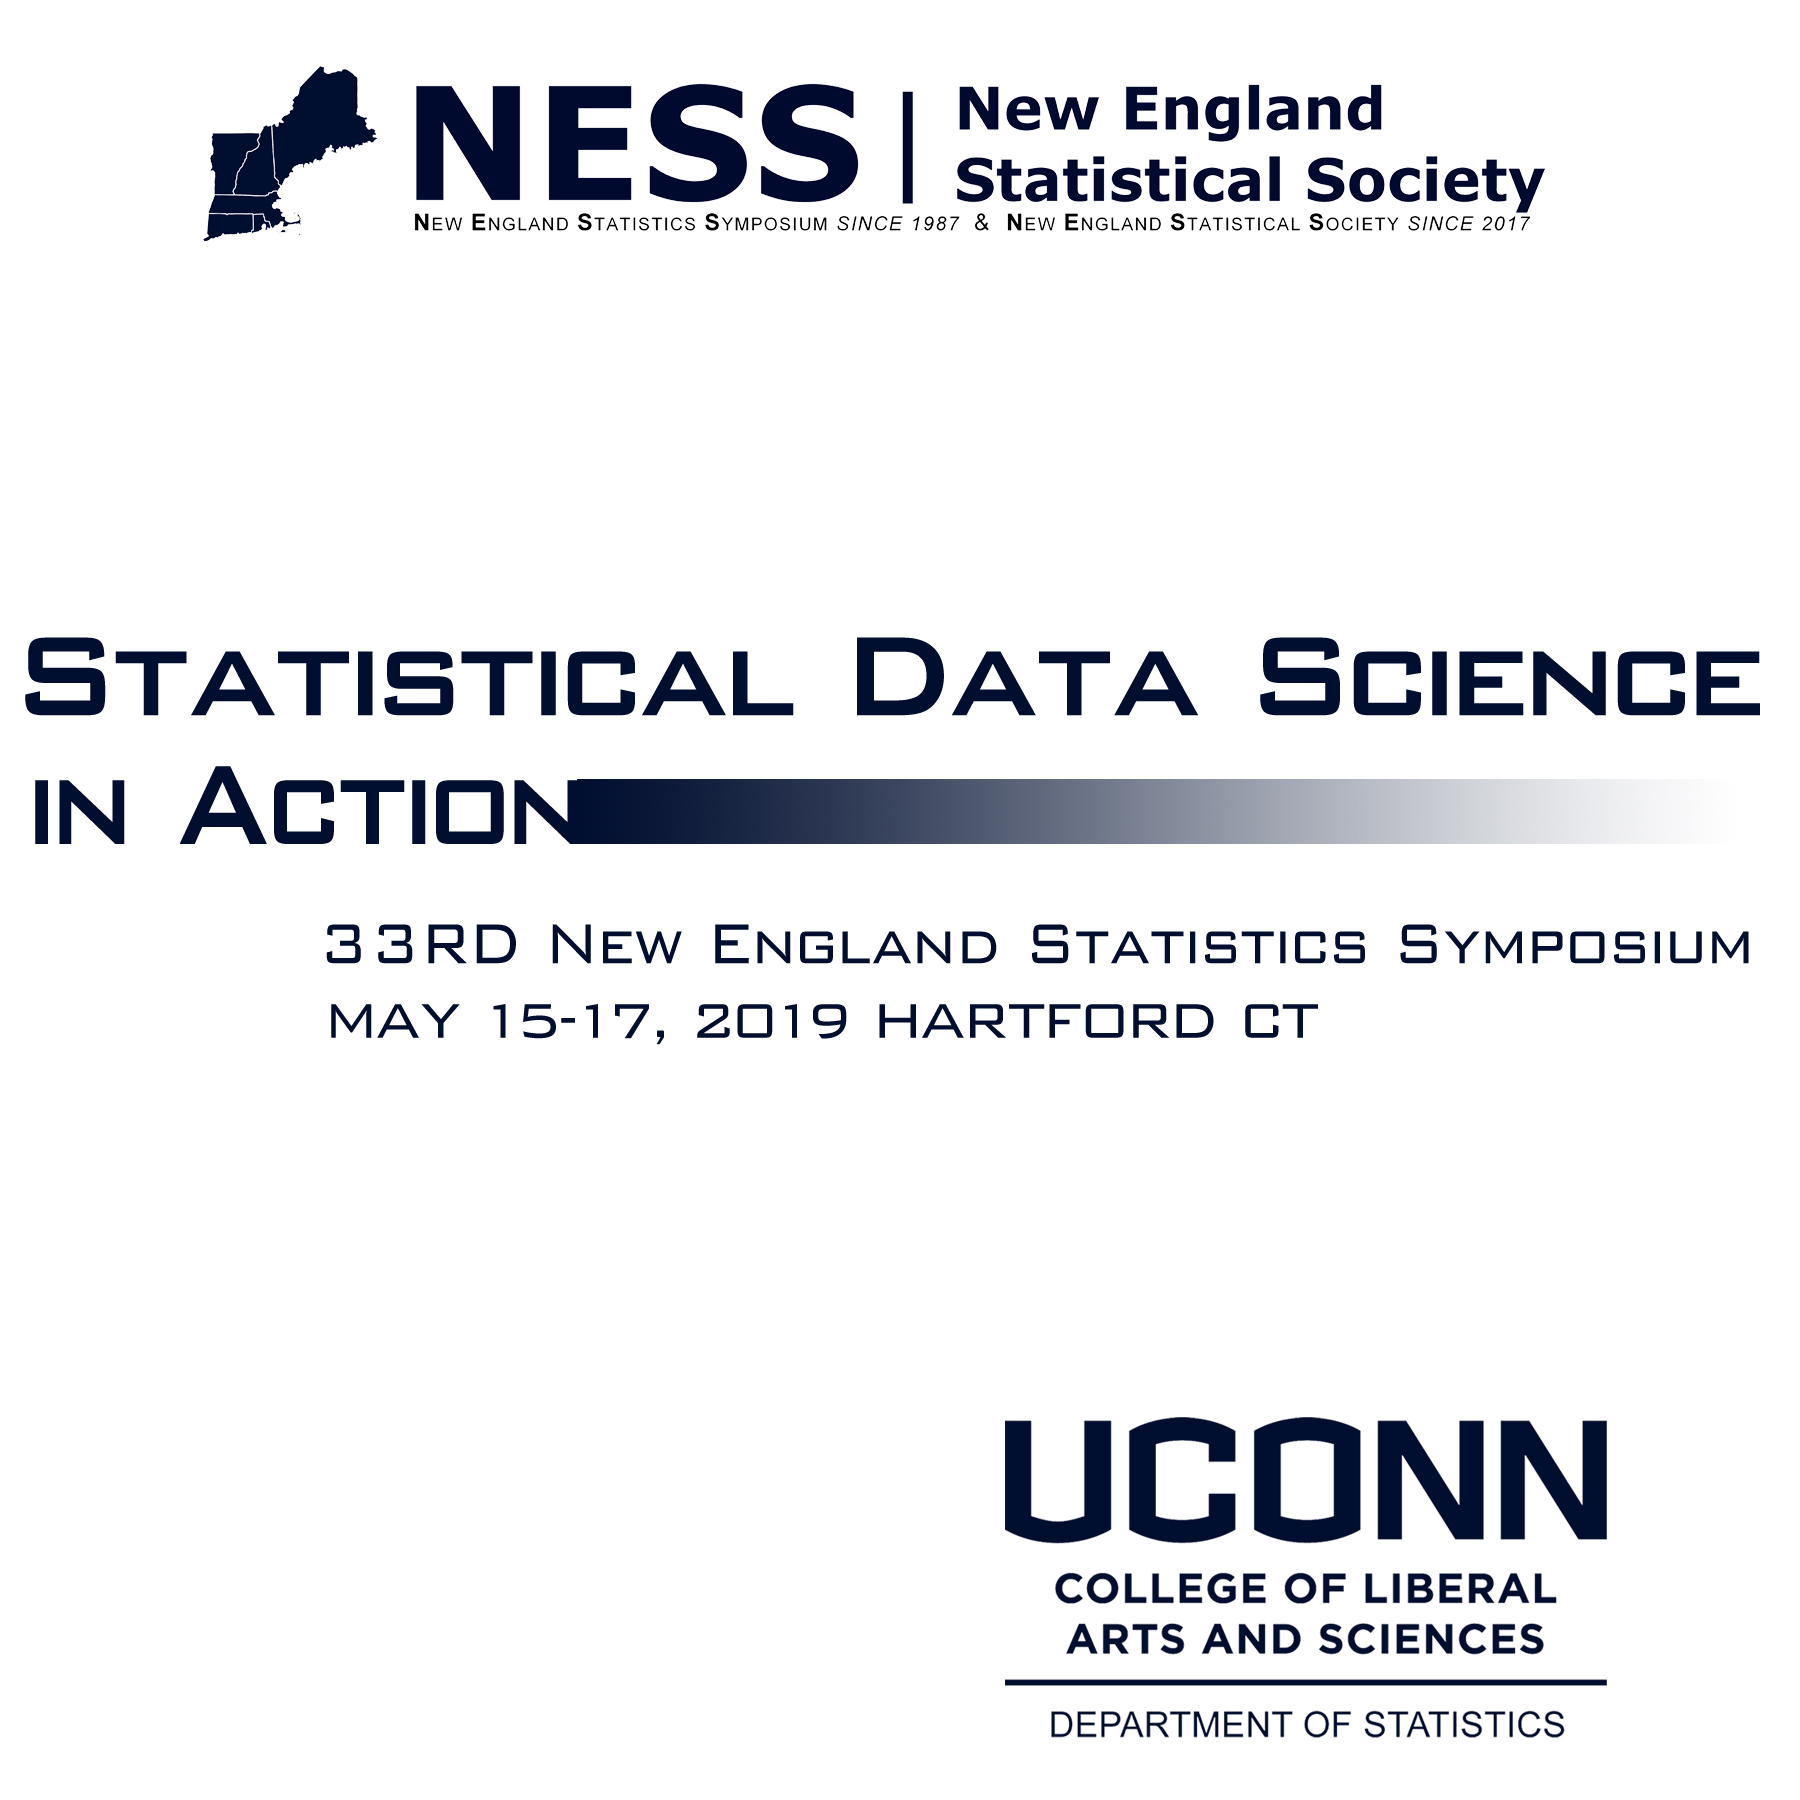
\includegraphics{bag.jpg}
\end{center}

\addcontentsline{toc}{section}{Cover}

\vfill

\clearpage


\section*{Conference Rooms/Floor Map}
\addcontentsline{toc}{section}{Conference Rooms/Floor Map}

The conference takes place on the 3 floors:

\vfill
\begin{itemize}
\item 2nd floor: Salon A; Salon B; Salon C
  \vfill
  \includegraphics[page=3, width=\textwidth, viewport=.23in 5.3in
  8.1in 9.07in, clip=true]{hilton.pdf}
  \vfill
\item 3rd floor: Mark Twain; Nathan Hale South; Nathan Hale North;
  Silas Deane; Colt; Wadsworth; Ethan Allen
  \vfill
  \includegraphics[page=3, width=\textwidth, viewport=.23in 1.66in
  8.1in 4.9in, clip=true]{hilton.pdf}
  \vfill
\item 6th floor: Saratoga A (which is one of the only two meeting rooms on this floor)
\end{itemize}

\vfill
All the plenary events and food/drink services are held in the Hilton
Ballroom on the 3rd floor.

\clearpage

\section*{\centering NESS 2019 Program}
% \addcontentsline{toc}{section}{Table of Contents}
{\centering \small \tableofcontents}

\clearpage


\section*{Plenary Speakers}
\addcontentsline{toc}{section}{Plenary Speakers}

\subsection*{Keynote Addresses: 9:10--10:45 am, Thursday, May 16}

\noindent
{\bf Big Data, Google and Disease Detection: A Statistical Adventure}

\emph{Dr. Samuel Kou, Harvard University}


Big data collected from the internet have generated significant
interest in not only the academic community but also industry and
government agencies. They bring great potential in tracking and
predicting massive social activities. We focus on tracking disease
epidemics in this talk. We will discuss the applications, in
particular, Google Flu Trends, some of the fallacy and the statistical
implications. We will propose a new model that utilizes publicly
available online data to estimate disease epidemics. Our model
outperforms all previous real-time tracking models for influenza
epidemics at the national level of the US. An extended version of the
model gives accurate tracking of Dengue fever in Asian and South
American countries. We will also draw some lessons for big data
applications.

{\bf Machine Learning for Structured and Unstructured Data in Finance}

\emph{Dr. David Rosenberg / Dr. Amanda Stent, Bloomberg}

Today's finance industry is continuously searching for alpha, through
more advanced modeling and through alternative sources of data. Many
alternative sources of data are not raw numerical data but structured
and unstructured documents - tables, graphics and text. In this talk,
we present ML methods for extracting information from documents. We
also present a case study of how such information can be combined with
market data for better predictive modeling.


\subsection*{Banquet Address:  Evening, Thursday, May 16, 2019}

\noindent
{\bf Improving Patient Outcomes in Prostate Cancer by Partnering
  Statistics and Medicine}

\emph{Dr. Anthony D'Amico, Dana-Farber Cancer Institute and Brigham \& Women's Hospital}

Several examples of how statistical methodology was used to improve
patient care and prostate cancer control outcomes will be discussed.


\subsection*{Chernoff Lecture: 3:10--4:20 pm, Friday, May 17}

Sorry, we do not who the inaugural Chernoff Awardee is. Come to the
closing plenary to find out!

\clearpage

\newgeometry{margin=0.75in}
\twocolumn
% \raggedright

\twocolumn[
\centering {\bf\Huge Detailed Program}
\bigskip
]
\addcontentsline{toc}{section}{Detailed Program}

\subsection*{Parallel Sessions: May 16, 11:00-12:40}
\addcontentsline{toc}{subsection}{Parallel Sessions: May 16, 11:00-12:40}

\vbox{\emph{Location: Saratoga A} \\ \subsubsection*{1. New Advances in Network Data Analysis}}
\addcontentsline{toc}{subsubsection}{New Advances in Network Data Analysis}

\begin{enumerate}[align=left]
\item [\emph{Organizer:}] \textbf{Guanyu Hu}, University of Connecticut
\item [\emph{Chair:}] \textbf{Lijiang Geng},  University of Connecticut
\end{enumerate}

\begin{itemize}
\item \textbf{Tracy Ke}, Harvard University \\
Optimal Adaptivity of Signed-Polygon Statistics for Network Testing
\item \textbf{Junxian Geng}, Boehringer Ingelheim \\
Probabilistic Community Detection with Unknown Number of Communities
\item \textbf{Vince Lyzinski}, University of Massachusetts Amherst \\
Matchability of Heterogeneous Networks Pairs
\item \textbf{Leo Duan}, University of Florida \\
Spiked Laplacian Graphs: Bayesian Modeling of Multiple Networks under Heterogeneity
\end{itemize}

\vspace{16pt}\vbox{\emph{Location: Salon C} \\ \subsubsection*{2. Mathematical Finance}}
\addcontentsline{toc}{subsubsection}{Mathematical Finance}

\begin{enumerate}[align=left]
\item [\emph{Organizer:}] \textbf{Oleksii Mostovyi}, University of Connecticut
\item [\emph{Chair:}] \textbf{Oleksii Mostovyi}, University of Connecticut
\end{enumerate}

\begin{itemize}
\item \textbf{Oleksii Mostovyi}, University of Connecticut \\
Asymptotic Analysis of the Expected Utility Maximization Problem with Respect to Perturbations of the Numeraire
\item \textbf{Hussein Nasralah}, Worcester Polytechnic Institute \\
Asymptotic Approximation of Optimal Portfolio for Small Time Horizons
\item \textbf{Sveinn Olafsson}, Columbia University \\
Adaptive Robo-Advising Framework
\item \textbf{Konstantinos Spiliopoulos}, Boston University \\
DGM: A Deep Learning Algorithm for Solving Partial Differential Equations
\end{itemize}

\vspace{16pt}\vbox{\emph{Location: Nathan Hale South} \\ \subsubsection*{3. Topics in Correlated and Clustered Data}}
\addcontentsline{toc}{subsubsection}{Topics in Correlated and Clustered Data}

\begin{enumerate}[align=left]
\item [\emph{Organizer:}] \textbf{Kerrie Nelson}, Department of Biostatistics, Boston University
\item [\emph{Chair:}] \textbf{Kerrie Nelson}, Department of Biostatistics, Boston University
\end{enumerate}

\begin{itemize}
\item \textbf{Tom Chen}, Harvard Pilgrim Healthcare and Harvard Medical School \\
Robust Estimation for Recurrent Event Analysis in the Presence of Informative Event Censoring
\item \textbf{Aya A. Mitani}, Boston University \\
Modeling Tooth-Loss using Inverse Probability Censoring Weights in Longitudinal Clustered Data with Informative Cluster Size
\item \textbf{Yorghos Tripodis}, Boston University School of Public Health \\
Dynamic Factor Analysis for Multivariate Time Series: An Application to Cognitive Trajectories
\item \textbf{Dongdong Li}, Harvard Medical School and Harvard Pilgrim Health Care Institute \\
Statistical Inference Using Large Administrative Data on Multiple Event Times, with Application to Cancer Survivorship Research
\end{itemize}

\vspace{16pt}\vbox{\emph{Location: Colt Boardroom} \\ \subsubsection*{4. Recent Advances in Design of Experiment}}
\addcontentsline{toc}{subsubsection}{Recent Advances in Design of Experiment}

\begin{enumerate}[align=left]
\item [\emph{Organizer:}] \textbf{Wei Zheng}, University of Tennessee
\item [\emph{Chair:}] \textbf{Wei Zheng}, University of Tennessee
\end{enumerate}

\begin{itemize}
\item \textbf{Qian Xiao}, University of Georgia \\
EzGP: Easy-to-Interpret Gaussian Process Models for Computer Experiments with Both Quantitative and Qualitative Factors
\item \textbf{Wanchunzi Yu}, Bridgewater State University \\
Robust Dose-Level Designs for Binary Responses in Environmental Risk Assessment
\item \textbf{Qiong Zhang}, Qiongz@clemson.edu \\
Sequential Data Collection for Stochastic Simulation Calibration
\item \textbf{Wei Zheng}, University of Tennessee \\
Design Based Incomplete U-Statistics
\end{itemize}

\vspace{16pt}\vbox{\emph{Location: Ethan Allen} \\ \subsubsection*{5. Statistical Methods for Big Data in Neuroscience}}
\addcontentsline{toc}{subsubsection}{Statistical Methods for Big Data in Neuroscience}

\begin{enumerate}[align=left]
\item [\emph{Organizer:}] \textbf{Jeff Goldsmith}, Columbia University, Department of Biostatistics
\item [\emph{Chair:}] \textbf{Jeff Goldsmith}, Columbia University, Department of Biostatistics
\end{enumerate}

\begin{itemize}
\item \textbf{Joanne C. Beer}, University of Pennsylvania \\
Harmonization of Multi-Scanner Longitudinal MRI Neuroimaging Data
\item \textbf{Adam Ciarleglio}, George Washington University \\
Handling Missing Clinical and Imaging Data in Integrative Analysis with Applications to Mental Health Research
\item \textbf{Elizabeth Sweeney}, Weill Cornell \\
Characterizing the Longitudinal Behavior of Multiple Sclerosis Lesions on Structural Magnetic Resonance Images
\item \textbf{Julia Wrobel}, Columbia University \\
Intensity Warping for Multisite MRI Normalization
\end{itemize}

\vspace{16pt}\vbox{\emph{Location: Wadsworth} \\ \subsubsection*{6. High Dimensional Dependent Data Analysis}}
\addcontentsline{toc}{subsubsection}{High Dimensional Dependent Data Analysis}

\begin{enumerate}[align=left]
\item [\emph{Organizer:}] \textbf{Yao Zheng}, Purdue University
\item [\emph{Chair:}] \textbf{Yao Zheng}, Purdue University
\end{enumerate}

\begin{itemize}
\item \textbf{Xianyang Zhang}, Texas A\&M University \\
A New Framework for Distance and Kernel-Based Metrics in High Dimensions
\item \textbf{Ruixuan Liu}, Emory University \\
Average Derivative Based Estimation of High Dimensional Single-Index Models
\item \textbf{Zeng Li}, The Pennsylvania State University \\
On Testing for High Dimensional White Noise
\item \textbf{Yao Zheng}, Purdue University \\
Finite Time Analysis of Vector Autoregressive Models under Linear Restrictions
\end{itemize}

\vspace{16pt}\vbox{\emph{Location: Nathan Hale North} \\ \subsubsection*{7. Causality, Inference, and Applications}}
\addcontentsline{toc}{subsubsection}{Causality, Inference, and Applications}

\begin{enumerate}[align=left]
\item [\emph{Organizer:}] \textbf{Tamara Broderick}, MIT
\item [\emph{Chair:}] \textbf{Tamara Broderick}, MIT
\end{enumerate}

\begin{itemize}
\item \textbf{Wenrui Li}, Boston University \\
Causal Inference under Network Interference with Noise
\item \textbf{Caroline Uhler}, Massachusetts Institute of Technology \\
From Causal Inference to Gene Regulation
\item \textbf{Youssef Marzouk}, Massachusetts Institute of Technology \\
Transportation for Inference in Non-Gaussian State Space Models
\item \textbf{Yicheng Kang}, Bentley University \\
Measuring Timeliness of Annual Reports Filing by Jump Additive Models
\end{itemize}

\vspace{16pt}\vbox{\emph{Location: Silas Deane} \\ \subsubsection*{8. Teaching Data Science}}
\addcontentsline{toc}{subsubsection}{Teaching Data Science}

\begin{enumerate}[align=left]
\item [\emph{Organizer:}] \textbf{D. Betsy Mccoach}, University of Connecticut
\item [\emph{Chair:}] \textbf{D. Betsy Mccoach}, University of Connecticut
\end{enumerate}

\begin{itemize}
\item \textbf{D. Betsy Mccoach}, University of Connecticut \\
Data Science Versus Statistics: What Do Students Need to Know?
\item \textbf{Randi Garcia}, Smith College \\
Integrating Real-World Research Projects in an Undergraduate Design and Analysis Course
\item \textbf{Eric D. Kolaczyk}, Boston University \\
Statistics Practicum @ Boston University
\end{itemize}

\vspace{16pt}\vbox{\emph{Location: Salon A} \\ \subsubsection*{9. Using Statistics for Health Delivery System Reform in Massachusetts}}
\addcontentsline{toc}{subsubsection}{Using Statistics for Health Delivery System Reform in Massachusetts}

\begin{enumerate}[align=left]
\item [\emph{Organizer:}] \textbf{Arlene Ash}, Dept of Population and Quantitative Health Sciences, University of Massachusetts Medical School
\item [\emph{Chair:}] \textbf{Arlene Ash}, Dept of Population and Quantitative Health Sciences, University of Massachusetts Medical School
\end{enumerate}

\begin{itemize}
\item \textbf{Eric Mick, ScD}, University of Massachusetts Medical School \\
Risk-Adjusted Quality Measure Model for Emergency Department Visits in Medicaid Adult Population with Severe Mental Illness and Substance Use Disorders
\item \textbf{Karen M Clements}, University of Massachusetts Medical School \\
Statistical Approaches to Evaluating Changes in Opioid Overdoses in Massachusetts: Challenges and Strategies
\item \textbf{Matthew Alcusky}, University of Massachusetts Medical School \\
Matching Payment to Need: Risk Adjusting Medicaid Payment for Long-Term Services and Supports in an Elderly Dual-Eligible Population
\item \textbf{Nien Chen Li}, Department of Quantitative Health Sciences, University of Massachusetts Medical School \\
Retention Within the Community as a Quality Measure for MassHealth Members with Behavioral Health Disorders
\end{itemize}

\vspace{16pt}\vbox{\emph{Location: Salon B} \\ \subsubsection*{10. Biomedical Data Science: To Infinity and Beyond!}}
\addcontentsline{toc}{subsubsection}{Biomedical Data Science: To Infinity and Beyond!}

\begin{enumerate}[align=left]
\item [\emph{Organizer:}] \textbf{Tor D. Tosteson}, Geisel School of Medicine at Dartmouth, Department of Biomedical Data Science
\item [\emph{Chair:}] \textbf{Tor D. Tosteson}, Geisel School of Medicine at Dartmouth, Department of Biomedical Data Science
\end{enumerate}

\begin{itemize}
\item \textbf{Erika Moen}, Geisel School of Medicine at Dartmouth \\
Network Analysis in Health Services Research: Opportunities and Challenges
\item \textbf{Jie Zhou}, Dartmouth College \\
Information Enhanced Model Selection for High-Dimensional Gaussian Graphical Model with Application to Metabolite Data
\item \textbf{Eugene Demidenko}, Dartmouth College \\
Machine Learning or Statistic? Machine Learning Enriched by Statistics
\item \textbf{Saeed Hassanpour}, Dartmouth College \\
Characterization of Histologic Patterns Using Deep Learning
\end{itemize}

\subsection*{Parallel Sessions: May 16, 14:00-15:40}
\addcontentsline{toc}{subsection}{Parallel Sessions: May 16, 14:00-15:40}

\vbox{\emph{Location: Ethan Allen} \\ \subsubsection*{11. High Dimensional Econometrics}}
\addcontentsline{toc}{subsubsection}{High Dimensional Econometrics}

\begin{enumerate}[align=left]
\item [\emph{Organizer:}] \textbf{Chihwa Kao}, University of Connecticut
\item [\emph{Chair:}] \textbf{Chihwa Kao}, University of Connecticut
\end{enumerate}

\begin{itemize}
\item \textbf{Fa Wang}, Cass Business School \\
Maximum Likelihood Estimation and Inference for High Dimensional Nonlinear Factor Models with Application to Factor-Augmented Regressions
\item \textbf{Yuan Liao}, Rutgers University \\
Inference for Heterogeneous Effects using Low Rank Estimations
\item \textbf{Min Seong Kim}, UConn \\
Policy Analysis Using Panel and Multilevel Models with Group Interactive Fixed Effects
\end{itemize}

\emph{Discussant:} \textbf{Jungbin Hwang}, UConn economics, jungbin.hwang@uconn.edu.

\vspace{16pt}\vbox{\emph{Location: Silas Deane} \\ \subsubsection*{12. Advances in Network and Algorithm Analysis}}
\addcontentsline{toc}{subsubsection}{Advances in Network and Algorithm Analysis}

\begin{enumerate}[align=left]
\item [\emph{Organizer:}] \textbf{Panpan Zhang}, University of Pennsylvania
\item [\emph{Chair:}] \textbf{Panpan Zhang}, University of Pennsylvania
\end{enumerate}

\begin{itemize}
\item \textbf{James Allen Fill}, The Johns Hopkins University, Department of Applied Mathematics and Statistics \\
Multivariate Pareto Records
\item \textbf{Wei-Chun Hung}, Johns Hopkins University \\
QuickSort: Improved Right-Tail Asymptotics for the Limiting Distribution, and Large Deviations
\item \textbf{Joshua Cape}, Johns Hopkins University \\
On Spectral Embedding Performance and Elucidating Network Structure in Stochastic Block Model Graphs
\item \textbf{Keith Levin}, University of Michigan \\
Bootstrapping Networks with Latent Space Structure
\end{itemize}

\vspace{16pt}\vbox{\emph{Location: Salon A} \\ \subsubsection*{13. Data Science in Actuarial Science}}
\addcontentsline{toc}{subsubsection}{Data Science in Actuarial Science}

\begin{enumerate}[align=left]
\item [\emph{Organizer:}] \textbf{Guojun Gan}, University of Connecticut
\item [\emph{Chair:}] \textbf{Guojun Gan}, University of Connecticut
\end{enumerate}

\begin{itemize}
\item \textbf{Jianxi Su}, Purdue University \\
Full-Range Tail Dependence Copulas for Modeling Dependent Insurance and Financial Data
\item \textbf{Thorsten Moenig}, Temple University \\
Negative Marginal Option Values:  the Interaction of Frictions and Option Exercise in Variable Annuities
\item \textbf{Zhiyu Quan}, University of Connecticut \\
Tree-Based Models for Variable Annuity Valuation: Parameter Tuning and Empirical Analysis
\item \textbf{Guojun Gan}, University of Connecticut \\
Nested Stochastic Valuation of Large Variable Annuity Portfolios: Monte Carlo Simulation and Synthetic Datasets
\end{itemize}

\vspace{16pt}\vbox{\emph{Location: Salon C} \\ \subsubsection*{14. Recent Advances and Applications of Measurement Error Models}}
\addcontentsline{toc}{subsubsection}{Recent Advances and Applications of Measurement Error Models}

\begin{enumerate}[align=left]
\item [\emph{Organizer:}] \textbf{Jeff Buzas}, University of Vermont
\item [\emph{Chair:}] \textbf{Jeff Buzas}, University of Vermont
\end{enumerate}

\begin{itemize}
\item \textbf{Donna Spiegelman}, Yale School of Public Health \\
Estimation and Inference in the Cox Model for Functions of the Covariate History when the Covariate is Measured with Error
\item \textbf{Brent A. Johnson}, University of Rochester \\
Monte Carlo Methods for Nonparametric Regression with Heteroscedastic Measurement Error
\item \textbf{Eugene Demidenko}, Dartmouth College \\
Who Said Pi?
\end{itemize}

\vspace{16pt}\vbox{\emph{Location: Colt Boardroom} \\ \subsubsection*{15. Recent Advances in Time Series Analysis and Diffusion Processes}}
\addcontentsline{toc}{subsubsection}{Recent Advances in Time Series Analysis and Diffusion Processes}

\begin{enumerate}[align=left]
\item [\emph{Organizer:}] \textbf{Ting Zhang}, Boston University
\item [\emph{Chair:}] \textbf{Ting Zhang}, Boston University
\end{enumerate}

\begin{itemize}
\item \textbf{Mamikon Ginovyan}, Boston University \\
Asymptotic Statistical Inference for Levy-Driven Continuous-Time Linear Models with Tapered Data
\item \textbf{Siragan M Gailus}, Boston University \\
Statistical Inference for Continuously- And Discretely-Observed Multiscale Diffusion Processes
\item \textbf{Ashis Gangopadhyay}, Department of Mathematics and Statistics, Boston University \\
A Self-Adjusted Model for Volatility Estimation of Financial Data
\item \textbf{Qiao Pan}, Boston University \\
Asymptotic Behavior of Optimal Weighting in Generalized Self Normalization for Time Series
\end{itemize}

\vspace{16pt}\vbox{\emph{Location: Wadsworth} \\ \subsubsection*{16. Modern Statistical Methods for Health Outcome Data}}
\addcontentsline{toc}{subsubsection}{Modern Statistical Methods for Health Outcome Data}

\begin{enumerate}[align=left]
\item [\emph{Organizer:}] \textbf{Jing Wu}, University of Rhode Island
\item [\emph{Chair:}] \textbf{Jing Wu}, University of Rhode Island
\end{enumerate}

\begin{itemize}
\item \textbf{Yan Zhuang}, Connecticut College \\
Two-Sample Sequential Methodologies for Tests of Hypotheses with Applications: Comparing Normal Means When the Two Variances are Unknown and Unequal
\item \textbf{Yichi Zhang}, University of Rhode Island \\
Prior Adaptive Semi-Supervised Learning with Application to Electronic Health Records Phenotyping
\item \textbf{Hao Li}, Boehringer Ingelheim Pharm Inc. \\
Bayesian Network Meta-Regression Hierarchical Models Using Heavy-Tailed Multivariate Random Effects with Covariate-Dependent Variances
\item \textbf{Yishu Xue}, Department of Statistics, University of Connecticut \\
Geographically Weighted Cox Regression for Prostate Cancer Survival Data in Louisiana
\end{itemize}

\vspace{16pt}\vbox{\emph{Location: Mark Twain} \\ \subsubsection*{17. Data Science and Statistics in Insurance}}
\addcontentsline{toc}{subsubsection}{Data Science and Statistics in Insurance}

\begin{enumerate}[align=left]
\item [\emph{Organizer:}] \textbf{Nathan Lally}, Hartford Steam Boiler (Munich Re)
\item [\emph{Chair:}] \textbf{Nathan Lally}, Hartford Steam Boiler (Munich Re)
\end{enumerate}

\begin{itemize}
\item \textbf{Brian Hartman}, Brigham Young University \\
Bayesian Multivariate Regime-Switching Models and the Impact of Correlation Structure Misspecification in Variable Annuity Pricing
\item \textbf{Shanshan Li}, MassMutual Data Science \\
Adjustment of Under-Reporting Bias in Mortality Studies
\item \textbf{Haimao Zhan}, MassMutual Financial Group \\
Data Science in Disability Insurance Claim Operations
\end{itemize}

\vspace{16pt}\vbox{\emph{Location: Nathan Hale South} \\ \subsubsection*{18. Healthcare Data Analysis for Electronic \\ Health Records}}
\addcontentsline{toc}{subsubsection}{Healthcare Data Analysis for Electronic Health Records}

\begin{enumerate}[align=left]
\item [\emph{Organizer:}] \textbf{Junwei Lu}, Harvard University
\item [\emph{Chair:}] \textbf{Junwei Lu}, Harvard University
\end{enumerate}

\begin{itemize}
\item \textbf{Xu Shi}, Harvard University \\
Bridging the Gap Between Noisy Healthcare Data and Knowledge: Automated Translation of Medical Terminology
\item \textbf{Rounak Dey}, Harvard TH Chan School of Public Health \\
A Fast and Accurate Algorithm to Test for Binary Phenotypes and Its Application to PheWAS
\item \textbf{Walter Dempsey}, Harvard University \\
The Stratified Micro-Randomized Trial Design:  Sample Size Considerations for Testing Nested Causal Effects of Time-Varying Treatment
\end{itemize}

\emph{Discussant:} \textbf{Junwei Lu}, Harvard University, junweilu@hsph.harvard.edu

\vspace{16pt}\vbox{\emph{Location: Salon B} \\ \subsubsection*{19. Causal Identification and Models for Time-Varying Interventions}}
\addcontentsline{toc}{subsubsection}{Causal Identification and Models for Time-Varying Interventions}

\begin{enumerate}[align=left]
\item [\emph{Organizer:}] \textbf{Xiaoxuan Cai}, School of Public Health, Yale University
\item [\emph{Chair:}] \textbf{Forrest Crawford},  Yale University
\end{enumerate}

\begin{itemize}
\item \textbf{Leah Comment}, Harvard University, Department of Biostatistics \\
Bayesian Data Fusion for Unmeasured Confounding
\item \textbf{Ilya Shpitser}, Johns Hopkins University \\
Estimation of Personalized Effects Associated with Causal Pathways
\item \textbf{Xiaoxuan Cai}, School of Public Health, Yale University \\
Non-Parametric Identification of Causal Intervention Effects under Contagion
\end{itemize}

\emph{Discussant:} \textbf{Forrest Crawford}, Yale University, forrest.crawford@yale.edu

\vspace{16pt}\vbox{\emph{Location: Saratoga A} \\ \subsubsection*{20. Predictive Modeling in Data Science: Methods and Applications}}
\addcontentsline{toc}{subsubsection}{Predictive Modeling in Data Science: Methods and Applications}

\begin{enumerate}[align=left]
\item [\emph{Organizer:}] \textbf{Stavroula A. Chrysanthopoulou}, Brown University School of Public Health
\item [\emph{Chair:}] \textbf{Stavroula A. Chrysanthopoulou}, Brown University School of Public Health
\end{enumerate}

\begin{itemize}
\item \textbf{Michael Wolfson}, University of Ottawa \\
Applying Dynamic Microsimulation to Understand Health Inequalities
\item \textbf{Jon Steingrimsson}, Brown University \\
Deep Learning with Time-to-Event Outcomes
\item \textbf{Petros Pechlivanoglou}, The Hospital for Sick Children \\
Using Microsimulation for Inference and Prediction in the Presence of Competing Risks and Recurrent Events: A Multistate Model Perspective
\item \textbf{Eric Jutkowitz}, Brown University \\
Societal, Medicare, Medicaid, and Family Cost of Dementia in the United States
\end{itemize}

\subsection*{Parallel Sessions: May 16, 16:00-17:40}
\addcontentsline{toc}{subsection}{Parallel Sessions: May 16, 16:00-17:40}

\vbox{\emph{Location: Colt Boardroom} \\ \subsubsection*{21. Frontiers in Sequential Analysis with Applications}}
\addcontentsline{toc}{subsubsection}{Frontiers in Sequential Analysis with Applications}

\begin{enumerate}[align=left]
\item [\emph{Organizer:}] \textbf{Aleksey Polunchenko}, Binghamton University
\item [\emph{Chair:}] \textbf{Aleksey Polunchenko}, Binghamton University
\end{enumerate}

\begin{itemize}
\item \textbf{Vasanthan Raghavan}, Qualcomm \\
Sequential Methods for 5G Wireless Communications
\item \textbf{Kexuan Li}, Binghamton University \\
On the Convergence Rate of the Quasi- To Stationary Distribution for the Shiryaev-Roberts Diffusion
\item \textbf{Nitis Mukhopadhyay}, Department of Statistics, University of Connecticut-Storrs, Connecticut \\
Sequential Confidence Intervals for an Exponential Mean (MTBF)
\item \textbf{Aleksey S. Polunchenko}, Binghamton University \\
On the Minimax Performance of the Generalized Shiryaev-Roberts Quickest Change-Point Detection Procedure in Continuous Time
\end{itemize}

\vspace{16pt}\vbox{\emph{Location: Ethan Allen} \\ \subsubsection*{22. Career Opportunities in Statistics and Data Sciences}}
\addcontentsline{toc}{subsubsection}{Career Opportunities in Statistics and Data Sciences}

\begin{enumerate}[align=left]
\item [\emph{Organizer:}] \textbf{Naitee Ting}, Boehringer Ingelheim Pharmaceuticals, Inc.
\item [\emph{Chair:}] \textbf{Naitee Ting}, Boehringer Ingelheim Pharmaceuticals, Inc.
\end{enumerate}

\begin{itemize}
\item \textbf{Lei Wang} \\
 Lotus Group, lei.wang@tlgcareers.com
\item \textbf{Kathleen T. Ziff} \\
 Travelers, KZIFF@travelers.com
\item \textbf{Jing Wul} \\
 University of Rhode Island, jing\_wu@uri.edu
\item \textbf{Zhenkui Zhang} \\
 Liberty Mutual, ZHENKUI.ZHANG@LibertyMutual.com
\item \textbf{Fama Yuchen} \\
 Hartford Steam Boiler - Munich Re, Yuchen\_Fama@hsb.com
\end{itemize}

\vspace{16pt}\vbox{\emph{Location: Nathan Hale North} \\ \subsubsection*{23. New Perspectives in Statistical Inference for Data with High Dimensionality}}
\addcontentsline{toc}{subsubsection}{New Perspectives in Statistical Inference for Data with High Dimensionality}

\begin{enumerate}[align=left]
\item [\emph{Organizer:}] \textbf{Wen Zhou}, Colorado State University
\item [\emph{Chair:}] \textbf{Haiying Wang},  University of Connecticut
\end{enumerate}

\begin{itemize}
\item \textbf{Byol Kim}, University of Chicago \\
Statistical Inference for the Difference of High-Dimensional Markov Random Fields via De-Biased Kullback-Leibler Importance Estimation Procedure (KLIEP)
\item \textbf{Wen Zhou}, Colorado State University \\
A Fusion Penalized Logistic Threshold Regression Model with Application to Diabetes Prognosis
\item \textbf{Kai Zhang}, UNC Chapel Hill \\
BET on Independence
\item \textbf{Ying Zhu}, Purdue University \\
Behavior of Lasso and Lasso-Based Inference under Limited Variability
\end{itemize}

\vspace{16pt}\vbox{\emph{Location: Silas Deane} \\ \subsubsection*{24. Some Applications of Statistics in Data Science}}
\addcontentsline{toc}{subsubsection}{Some Applications of Statistics in Data Science}

\begin{enumerate}[align=left]
\item [\emph{Organizer:}] \textbf{Balgobin Nandram}, Worcester Polytechnic Institute
\item [\emph{Chair:}] \textbf{Jian Zou},  Worcester Polytechnic Institute
\end{enumerate}

\begin{itemize}
\item \textbf{Andreea Luisa Erciulescu}, Westat \\
The Data Science Challenge of Bridging Two Complex Surveys
\item \textbf{Lu Chen}, National Institute of Statistical Sciences \\
Hierarchical Bayesian Logistic Regression Model for Sub-Areas
\item \textbf{Buddika Peiris}, Worcester Polytechnic Institute \\
An Improved Meta-Analysis for Analyzing Time Series Circular Regression with Application to Environmental Study
\item \textbf{Seongho Song}, University of Cincinnati \\
Hierarchical Bayesian Analysis for Stochastic Frontier Production Function Model
\end{itemize}

\vspace{16pt}\vbox{\emph{Location: Salon A} \\ \subsubsection*{25. Statistical Methodology for Healthcare Data Analysis}}
\addcontentsline{toc}{subsubsection}{Statistical Methodology for Healthcare Data Analysis}

\begin{enumerate}[align=left]
\item [\emph{Organizer:}] \textbf{Chongliang Luo}, University of Pennsylvania
\item [\emph{Chair:}] \textbf{Chongliang Luo}, University of Pennsylvania
\end{enumerate}

\begin{itemize}
\item \textbf{Grace Yi}, University of Waterloo \\
Analysis of Multi-State Models with Misclassified States
\item \textbf{Jing Huang}, University of Pennsylvania \\
PIE: A Prior Knowledge Guided Estimation Method for Bias Reduction in EHR-Based Research
\item \textbf{Peng Wu}, Columbia University \\
Matched Learning for Optimizing Individualized Treatment Strategies Using Electronic Health Records
\item \textbf{Chongliang Luo}, University of Pennsylvania \\
An Augmented Survival Analysis Method for Interval Censored and Mis-Measured Outcomes
\end{itemize}

\vspace{16pt}\vbox{\emph{Location: Nathan Hale South} \\ \subsubsection*{26. New Developments of Several Classical Statistical Methods}}
\addcontentsline{toc}{subsubsection}{New Developments of Several Classical Statistical Methods}

\begin{enumerate}[align=left]
\item [\emph{Organizer:}] \textbf{Yuwen Gu}, University of Connecticut
\item [\emph{Chair:}] \textbf{Yuwen Gu}, University of Connecticut
\end{enumerate}

\begin{itemize}
\item \textbf{Chenglong Ye}, University of Minnesota \\
High-Dimensional Adaptive Minimax Sparse Estimation with Interactions
\item \textbf{Megan Heyman}, Rose-Hulman Institute of Technology \\
Bootstrap in Linear Models:  a Comprehensive R Package
\item \textbf{Boxiang Wang}, University of Iowa \\
Magic Cross-Validation for Support Vector Machines and Related Large Margin Classifiers
\item \textbf{Dootika Vats}, University of Warwick \\
Revisiting the Gelman-Rubin Diagnostic
\end{itemize}

\vspace{16pt}\vbox{\emph{Location: Mark Twain} \\ \subsubsection*{27. Estimating and Hypothesis Testing in Time Series and Spatial Models}}
\addcontentsline{toc}{subsubsection}{Estimating and Hypothesis Testing in Time Series and Spatial Models}

\begin{enumerate}[align=left]
\item [\emph{Organizer:}] \textbf{Yu (Ryan) Yue}, Baruch College, the City University of New York
\item [\emph{Chair:}] \textbf{Yu (Ryan) Yue}, Baruch College, the City University of New York
\end{enumerate}

\begin{itemize}
\item \textbf{Zeda Li}, Baruch College CUNY \\
Model-Free Variable Selection with Matrix-Valued Predictors
\item \textbf{Zifei Han}, Vertex Pharmaceuticals \\
Gaussian Copula Models for Geostatistical Count Data: Estimation and Prediction
\item \textbf{Rongning Wu}, The City University of New York \\
Least Tail-Trimmed Absolute Deviation Estimation for Autoregressions with Infinite/Finite Variance
\item \textbf{Victor Pena}, Baruch College (CUNY) \\
Crteria for Bayesian Hypothesis Testing in Two-Sample Problems
\end{itemize}

\vspace{16pt}\vbox{\emph{Location: Saratoga A} \\ \subsubsection*{28. Bayesian Method and Causal Inference}}
\addcontentsline{toc}{subsubsection}{Bayesian Method and Causal Inference}

\begin{enumerate}[align=left]
\item [\emph{Organizer:}] \textbf{Ting Zhang}, Boston University
\item [\emph{Chair:}] \textbf{Siragan Gailus (Siragan@bu.edu)},  Boston University
\end{enumerate}

\begin{itemize}
\item \textbf{Gautam Sabnis}, Boston University \\
Bayesian Variable Selection in Linear Regression Models with Instrumental Variables
\item \textbf{Julio Enrique Castrillon}, Boston University \\
Large Scale Kriging: A High Performance Multi-Level Computational Mathematics Approach
\item \textbf{Luis Carvalho}, Boston University \\
Invariant Objective Bayesian Priors for Linear Models
\item \textbf{Joonha Park}, Boston University \\
Sequential Proposal Markov Chain Monte Carlo Sampling Algorithms
\end{itemize}

\vspace{16pt}\vbox{\emph{Location: Salon C} \\ \subsubsection*{29. Critical Questions in Drug Development}}
\addcontentsline{toc}{subsubsection}{Critical Questions in Drug Development}

\begin{enumerate}[align=left]
\item [\emph{Organizer:}] \textbf{Jie Tang}, FMD K\&L Inc
\item [\emph{Chair:}] \textbf{Jie Tang}, FMD K\&L Inc
\end{enumerate}

\begin{itemize}
\item \textbf{Jie Tang}, FMD K\&L Inc \\
Critical Questions in Drug Development, a Phase 3 Vaccine Study using Group-Sequential Design with Blinded Sample Size Re-Estimation
\item \textbf{Cassie Dong}, Seattle Genetics \\
Clinical Bridging Study Design using Frequentist and Bayesian Methods
\item \textbf{Xiang Li}, Janssen Research \& Development, LLC \\
Coupling Machine Learning with Empirical Bayes Estimates from Mixed-Effects Modeling for High-Throughput and Efficient Feature Selection for Longitudinal Disease Dynamic Data with High-Dimensional Prognostic Biomarkers
\end{itemize}

\emph{Discussant:} \textbf{Naitee Ting}, Boehringer Ingelheim

\vspace{16pt}\vbox{\emph{Location: Wadsworth} \\ \subsubsection*{30. New Developments on Data Compatibility and Related  Topics}}
\addcontentsline{toc}{subsubsection}{New Developments on Data Compatibility and Related  Topics}

\begin{enumerate}[align=left]
\item [\emph{Organizer:}] \textbf{Lynn Kuo}, University of Connecticut
\item [\emph{Chair:}] \textbf{Lynn Kuo}, University of Connecticut
\end{enumerate}

\begin{itemize}
\item \textbf{Daoyuan Shi}, Vertex Pharmaceuticals \\
Data Compatibility in Drug Development
\item \textbf{Wei Shi}, Department of Statistics, University of Connecticut \\
New Bayesian Measures for Information and Data Compatibility
\item \textbf{Yu-Bo Wang}, Clemson University \\
Bayesian Assessment of the Joint, Marginal and Conditional Information Gains with Applications
\item \textbf{Guanyu Hu}, University of Connecticut \\
New Development of Bayesian Variable Selection Criteria for Spatial Point Process with Applications
\end{itemize}

\subsection*{Parallel Sessions: May 17, 08:30-10:10}
\addcontentsline{toc}{subsection}{Parallel Sessions: May 17, 08:30-10:10}

\vbox{\emph{Location: Mark Twain} \\ \subsubsection*{31. Computationally Efficient Statistical Methods for Inference on Data with Complex Structures}}
\addcontentsline{toc}{subsubsection}{Computationally Efficient Statistical Methods for Inference on Data with Complex Structures}

\begin{enumerate}[align=left]
\item [\emph{Organizer:}] \textbf{Wen Zhou}, Colorado State University
\item [\emph{Chair:}] \textbf{Yuwen Gu},  University of Connecticut
\end{enumerate}

\begin{itemize}
\item \textbf{Danning Li}, Penn State University \\
Hypothesis Testing for Community Detection in Stochastic Block Models
\item \textbf{Bharath Sriperumbudur}, Pennsylvania State Univeristy \\
Approximate Kernel PCA: Computational vs. Statistical Trade-Off
\item \textbf{Cynthia Rush}, Columbia University \\
Approximate Message Passing Algorithms for High-Dimensional Statistical Estimation
\item \textbf{Daniel L Sussman}, Boston University \\
Joint Network Embeddings: Bias, Regression, and Testing
\end{itemize}

\vspace{16pt}\vbox{\emph{Location: Colt Boardroom} \\ \subsubsection*{32. Flexible Modeling of Censored Data}}
\addcontentsline{toc}{subsubsection}{Flexible Modeling of Censored Data}

\begin{enumerate}[align=left]
\item [\emph{Organizer:}] \textbf{Victor Hugo Lachos Davila}, Department of Statistics, University of Connecticut
\item [\emph{Chair:}] \textbf{Jorge Luis Bazan Guzman}
\end{enumerate}

\begin{itemize}
\item \textbf{Christian E Galarza}, Campinas State University \\
On Moments of Truncated Multivariate Skew-Normal Distribution with Applications in Interval Censored Data
\item \textbf{Thalita Do Bem Mattos}, University of Campinas \\
A Semiparametric Mixed-Effects Model for Longitudinal  Censored Data
\item \textbf{Francisco Hildemar Calixto de Alencar}, State University of Campinas \\
Finite Mixture of Censored Linear Mixed Models for Longitudinal Data
\item \textbf{Larissa Avila Matos}, Universidade Estadual De Campinas \\
Linear Mixed Models for Multiple Censored Responses Data
\end{itemize}

\vspace{16pt}\vbox{\emph{Location: Nathan Hale South} \\ \subsubsection*{33. Bayesian Methods and Applications}}
\addcontentsline{toc}{subsubsection}{Bayesian Methods and Applications}

\begin{enumerate}[align=left]
\item [\emph{Organizer:}] \textbf{Tevfik Aktekin}, University of New Hampshire
\item [\emph{Chair:}] \textbf{Tevfik Aktekin}, University of New Hampshire
\end{enumerate}

\begin{itemize}
\item \textbf{Nalini Ravishanker}, University of Connecticut \\
Modeling Vector Time Series of Counts
\item \textbf{Christopher Glynn}, University of New Hampshire \\
Inflection Points in Community-Level Homeless Rates
\item \textbf{Tevfik Aktekin}, University of New Hampshire \\
A Bayesian Family of Multivariate Non-Gaussian State Space Models
\item \textbf{Panpan Zhang}, University of Pennsylvania \\
Community Detection in Social Networks
\end{itemize}

\vspace{16pt}\vbox{\emph{Location: Silas Deane} \\ \subsubsection*{34. Recent Advances in Statistical Methods for Missing or Truncated Data}}
\addcontentsline{toc}{subsubsection}{Recent Advances in Statistical Methods for Missing or Truncated Data}

\begin{enumerate}[align=left]
\item [\emph{Organizer:}] \textbf{Jing Qian}, University of Massachusetts, Amherst
\item [\emph{Chair:}] \textbf{Jing Qian}, University of Massachusetts, Amherst
\end{enumerate}

\begin{itemize}
\item \textbf{Sy Han Chiou}, University of Texas at Dallas \\
Permutation Tests for General Dependent Truncation
\item \textbf{Chi Hyun Lee}, University of Massachusetts Amherst \\
Analysis of Combined Incident and Prevalent Cohort Data under a Proportional Mean Residual Life Model
\item \textbf{Bella Vakulenko-Lagun}, Harvard University \\
Nonidentifiability in the Presence of Factorization for Truncated Data
\item \textbf{Zhichao Jiang}, Harvard University \\
Using Missing Types to Improve Partial Identification with Missing Binary Outcomes
\end{itemize}

\vspace{16pt}\vbox{\emph{Location: Saratoga A} \\ \subsubsection*{35. Novel Statistical Methods for the Analysis of Genomic Data}}
\addcontentsline{toc}{subsubsection}{Novel Statistical Methods for the Analysis of Genomic Data}

\begin{enumerate}[align=left]
\item [\emph{Organizer:}] \textbf{Elizabeth Schifano}, University of Connecticut
\item [\emph{Chair:}] \textbf{Elizabeth Schifano}, University of \\Connecticut
\end{enumerate}

\begin{itemize}
\item \textbf{Tamar Sofer}, Harvard Medical School \\
Carriers-Only Tests of Association of a Rare Genetic Variant with a Binary Outcome
\item \textbf{Iuliana Ionita-Laza}, Columbia University \\
Integrative Statistical Approaches for the Analysis of Whole-Genome Sequencing Data
\item \textbf{Lorin Crawford}, Brown University \\
Detecting Genetic Interactions with the Marginal Epistasis Test
\item \textbf{Zuoheng Wang}, Yale University \\
Identification of Trans-eQTLs Using Mediation Analysis with Multiple Mediators
\end{itemize}

\vspace{16pt}\vbox{\emph{Location: Ethan Allen} \\ \subsubsection*{36. Effective Communication of Technical Concepts to Non-Technical Audiences}}
\addcontentsline{toc}{subsubsection}{Effective Communication of Technical Concepts to Non-Technical Audiences}

\begin{enumerate}[align=left]
\item [\emph{Organizer:}] \textbf{Kathy Ziff}, Travelers Insurance
\item [\emph{Chair:}] \textbf{Chris Parks},  Travelers
\end{enumerate}

\begin{itemize}
\item \textbf{Eugene Evans} \\
 The Travelers Companies
\item \textbf{Chris Parks} \\
 The Travelers Companies
\item \textbf{Jiafeng Sun},  Ph.D. \\
 FCAS, The Travelers Companies
\item \textbf{Kathy Ziff} \\
 The Travelers Companies
\end{itemize}

\vspace{16pt}\vbox{\emph{Location: Salon C} \\ \subsubsection*{37. Application of Statistics and Data Sciences in Pharmaceutical Research and Development}}
\addcontentsline{toc}{subsubsection}{Application of Statistics and Data Sciences in Pharmaceutical Research and Development}

\begin{enumerate}[align=left]
\item [\emph{Organizer:}] \textbf{John Zhong}, Biogen, Inc.
\item [\emph{Chair:}] \textbf{John Zhong}, Biogen, Inc.
\end{enumerate}

\begin{itemize}
\item \textbf{Dawei Liu}, Biogen \\
Variable Importance Ranking with Confounder-Adjustment in Random Forest Based Survival Analysis
\item \textbf{Yingying Liu}, Biogen Inc. \\
Comparing Joint Rank, Trimmed-Mean and Jump-to-Control for Analyzing Clinical Trial Data with Missingness Due to Death
\item \textbf{Shijia Bian}, Global Analytics and Data Sciences, Biogen \\
Statistics and Data Science in Clinical Trial Operation and Clinical Data Quality Monitoring
\item \textbf{Fan Wu}, Biogen \\
A Working Model for Reproducible Analysis with Applications in Propensity Score Matching
\end{itemize}

\vspace{16pt}\vbox{\emph{Location: Nathan Hale North} \\ \subsubsection*{38. High-Dimensional Statistical Inference and Learning}}
\addcontentsline{toc}{subsubsection}{High-Dimensional Statistical Inference and Learning}

\begin{enumerate}[align=left]
\item [\emph{Organizer:}] \textbf{Yuping Zhang}, University of Connecticut
\item [\emph{Chair:}] \textbf{Yuping Zhang}, University of Connecticut
\end{enumerate}

\begin{itemize}
\item \textbf{Zhou Fan}, Yale University \\
Estimating Gradient-Sparse Signals from Linear Measurements
\item \textbf{Yihong Wu}, Yale University \\
Efficient Random Graph Matching via Degree Profiles
\item \textbf{Junwei Lu}, Harvard University \\
Combinatorial Inference
\item \textbf{Michael Kane}, Yale University \\
Graphical Model Approaches to Integrating Cell Tower and Spatial Data
\end{itemize}

\vspace{16pt}\vbox{\emph{Location: Wadsworth} \\ \subsubsection*{39. Data Science: Computational Social Science?}}
\addcontentsline{toc}{subsubsection}{Data Science: Computational Social Science?}

\begin{enumerate}[align=left]
\item [\emph{Organizer:}] \textbf{Dakota Cintron}, University of Connecticut
\item [\emph{Chair:}] \textbf{Dakota Cintron}, University of Connecticut
\end{enumerate}

\begin{itemize}
\item \textbf{Dakota Cintron}, University of Connecticut \\
Data Science as Computational Social Science
\item \textbf{D. Betsy Mccoach}, University of Connecticut \\
Big Social Science Data
\item \textbf{Mora Reinka}, University of Connecticut \\
Statistical Inference in Computational Social Science: A Sentiment Analysis Approach
\end{itemize}

\emph{Discussant:} \textbf{Devin Kearns}, University of Connecticut, devin.kearns@uconn.edu

\vspace{16pt}\vbox{\emph{Location: Salon B} \\ \subsubsection*{40. Advancement in the Marked-Point Process Modeling Framework for Real-Time Neural Data Analysis}}
\addcontentsline{toc}{subsubsection}{Advancement in the Marked-Point Process Modeling Framework for Real-Time Neural Data Analysis}

\begin{enumerate}[align=left]
\item [\emph{Organizer:}] \textbf{Ali Yousefi}, Postdoctoral Fellow
\item [\emph{Chair:}] \textbf{Uri T Eden},  Boston University
\end{enumerate}

\begin{itemize}
\item \textbf{Uri Eden}, Boston University \\
Marked Point Process Modeling and Estimation Problems in Neural Data Analysis: a Case Study
\item \textbf{Ali Yousefi}, Boston University, Department of Mathematics and Statistics \\
Assessing Goodness of Fit in Marked-Point Process Models
\item \textbf{Kensuke Arai}, Boston University Department of Mathematics and Statistics \\
Marked Point Process Filter for Clusterless and Adaptive Encoding-Decoding of Multiunit Activity
\item \textbf{Eric L. Denovellis}, Boston University \\
Using State Space Models to Identify Latent Temporal Dynamics of Population Spiking Activity.
\end{itemize}

\vspace{16pt}\vbox{\emph{Location: Salon A} \\ \subsubsection*{41. Statistical Learning Methods and Developments}}
\addcontentsline{toc}{subsubsection}{Statistical Learning Methods and Developments}

\begin{enumerate}[align=left]
\item [\emph{Organizer:}] \textbf{Minge Xie}, Rutgers University
\item [\emph{Chair:}] \textbf{Minge Xie}, Rutgers University
\end{enumerate}

\begin{itemize}
\item \textbf{Jason M. Klusowski}, Rutgers University - New Brunswick \\
Is it Possible to Motivate Tree-Based Measures of Variable Importance?
\item \textbf{Qiyang Han}, Rutgers University \\
Limit Distribution Theory for Multiple Isotonic Regression
\item \textbf{Guoqing Diao}, George Mason University \\
High Dimensional Covariate-Adjusted Semiparametric Transformation Gaussian Graphical Models
\item \textbf{Samory Kpotufe}, Columbia University \\
Measuring Transferability: some Recent Insights
\end{itemize}

\subsection*{Parallel Sessions: May 17, 10:30-12:10}
\addcontentsline{toc}{subsection}{Parallel Sessions: May 17, 10:30-12:10}

\vbox{\emph{Location: Saratoga A} \\ \subsubsection*{42. Statistical and Machine Learning Methods for Large-Scale Biomedical Data Analysis}}
\addcontentsline{toc}{subsubsection}{Statistical and Machine Learning Methods for Large-Scale Biomedical Data Analysis}

\begin{enumerate}[align=left]
\item [\emph{Organizer:}] \textbf{Zhengqing Ouyang}, The Jackson Laboratory for Genomic Medicine
\item [\emph{Chair:}] \textbf{Zhengqing Ouyang}, The Jackson Laboratory for Genomic Medicine
\end{enumerate}

\begin{itemize}
\item \textbf{Ion Mandoiu}, University of Connecticut \\
SC1: A Web-Based Single Cell RNA-Seq Analysis Pipeline
\item \textbf{Nicholas Reich}, UMass Biostatistics \\
Forecasting Infectious Disease Epidemics via Stacked Density Ensembles
\item \textbf{Donghui Yan}, UMass Dartmouth \\
Random Projection Forests with Applications to Biomedical Studies
\end{itemize}

\vspace{16pt}\vbox{\emph{Location: Silas Deane} \\ \subsubsection*{43. Applications of Network Science and Causal Inference Methods in Public Health Data}}
\addcontentsline{toc}{subsubsection}{Applications of Network Science and Causal Inference Methods in Public Health Data}

\begin{enumerate}[align=left]
\item [\emph{Organizer:}] \textbf{Natallia V. Katenka}, Department of Computer Science and Statistics, University of Rhode Island
\item [\emph{Chair:}] \textbf{Ben Skov}
\end{enumerate}

\begin{itemize}
\item \textbf{Isabel Fulcher}, Harvard University \\
Bayesian Auto-g-Computation of Network Causal Effects: Incarceration and Infection in a High Risk Network
\item \textbf{Olga Morozova}, Yale School of Public Health, Department of Biostatistics \\
Individualistic Intervention Effects Under Interference
\item \textbf{Natallia V. Katenka}, University of Rhode Island, Department of Computer Science and Statistics \\
Toward Evaluation of Dissemination of HIV Prevention Interventions Among Networks of People Who Inject Drugs
\item \textbf{Hilary A Aroke}, University of Rhode Island \\
Social Network Analysis of an Opioid Provider-Sharing Network of Patients
\end{itemize}

\vspace{16pt}\vbox{\emph{Location: Mark Twain} \\ \subsubsection*{44. Novel Computational Approaches for Analyzing Time Series}}
\addcontentsline{toc}{subsubsection}{Novel Computational Approaches for Analyzing Time Series}

\begin{enumerate}[align=left]
\item [\emph{Organizer:}] \textbf{Nalini Ravishanker}, University of Connecticut
\item [\emph{Chair:}] \textbf{Nalini Ravishanker}, University of Connecticut
\end{enumerate}

\begin{itemize}
\item \textbf{Jonathan Hosking}, Amazon.com \\
Analytical Likelihood Derivatives for State Space Forecasting Models
\item \textbf{M. Henry Linder}, University of Connecticut \\
Structural Break Detection for Utility Demand Monitoring at UCONN
\item \textbf{Haitao Liu}, Worcester Polytechnic Institute \\
Novel Computational Approaches for Analyzing Time Series
\item \textbf{Yue Tang}, Pratt\&Whitney \\
Application of Functional Principal Component Analysis (fPCA) in Identifying Gas Turbine Rotor Vibratory Characteristics
\end{itemize}

\vspace{16pt}\vbox{\emph{Location: Colt Boardroom} \\ \subsubsection*{45. Manifolds and Anomalies for Data Science}}
\addcontentsline{toc}{subsubsection}{Manifolds and Anomalies for Data Science}

\begin{enumerate}[align=left]
\item [\emph{Organizer:}] \textbf{Randy Paffenroth}, Worcester Polytechnic Institute
\item [\emph{Chair:}] \textbf{Randy Paffenroth}, Worcester Polytechnic Institute
\end{enumerate}

\begin{itemize}
\item \textbf{Randy Paffenroth}, Worcester Polytechnic Institute \\
Musings on Robust Dimensionality Reduction and Deep Learning
\item \textbf{Jian Zou}, Worcester Polytechnic Institute \\
Learning Low-Dimensional Manifolds for the Scoring of Tissue Microarray Images
\item \textbf{Aidong (Adam) Ding}, Northeastern University \\
Quantifying Probability of Adversarial Examples in Linear Classification
\item \textbf{Melanie Jutras}, The MITRE Corporation \\
Utilizing Matrix Norms for Dimension Reduction and Feature Selection
\end{itemize}

\vspace{16pt}\vbox{\emph{Location: Salon B} \\ \subsubsection*{46. Advances in Modeling and Computation for Latent Variable Models}}
\addcontentsline{toc}{subsubsection}{Advances in Modeling and Computation for Latent Variable Models}

\begin{enumerate}[align=left]
\item [\emph{Organizer:}] \textbf{Xiaojing Wang}, University of Connecticut
\item [\emph{Chair:}] \textbf{Xiaojing Wang}, University of Connecticut
\end{enumerate}

\begin{itemize}
\item \textbf{Zheng Wei}, University of Maine \\
Parallel Markov Chain Monte Carlo Method for Latent Variable Models-Bayesian Dynamic Item Response Models in Educational Testing
\item \textbf{Jorge Luis Bazan Guzman}, USP-UCONN \\
A Bayesian Cognitive Diagnosis Model for Continuous Response
\item \textbf{Jingchen Liu}, Columbia University, Department of Statistics \\
An Exploration of Latent Structure in Process Data
\item \textbf{Xiaojing Wang}, University of Connecticut \\
Bayesian Nonparametric Monotone Regression of Dynamic Latent Traits in Item Response Theory Models
\end{itemize}

\vspace{16pt}\vbox{\emph{Location: Wadsworth} \\ \subsubsection*{47. Air Pollution and Public Health: New Spatial and Spatio-Temporal Statistical Approaches for Exposure Assessment and Causal Inference}}
\addcontentsline{toc}{subsubsection}{Air Pollution and Public Health: New Spatial and Spatio-Temporal Statistical Approaches for Exposure Assessment and Causal Inference}

\begin{enumerate}[align=left]
\item [\emph{Organizer:}] \textbf{Veronica Berrocal}, University of Michigan, Department of Biostatistics
\item [\emph{Chair:}] \textbf{Gavino Puggioni},  University of Rhode Island
\end{enumerate}

\begin{itemize}
\item \textbf{Owais Gilani}, Bucknell University \\
Non-Stationary Spatiotemporal Bayesian Data Fusion for Pollutants in the Near-Road Environment
\item \textbf{Howard Chang}, Emory University \\
Statistical Methods for Combining Multiple Data Sources to Estimate Ambient Air Quality
\item \textbf{Alexandra Larsen}, Duke University \\
Environmental Statistics for Wildfire Management and Public Health
\item \textbf{Philip Andrew White}, Brigham Young University/Duke University \\
Multivariate Functional Factor Models with Time-Varying Clustering
\end{itemize}

\vspace{16pt}\vbox{\emph{Location: Salon A} \\ \subsubsection*{48. Sports Analytics}}
\addcontentsline{toc}{subsubsection}{Sports Analytics}

\begin{enumerate}[align=left]
\item [\emph{Organizer:}] \textbf{Gregory J. Matthews}, Loyola University Chicago
\item [\emph{Chair:}] \textbf{Gregory J. Matthews}, Loyola University Chicago
\end{enumerate}

\begin{itemize}
\item \textbf{Jieying Jiao}, University of Connecticut \\
A Bayesian Joint Model of Mark and Intensity of Marked   Spatial Point Processes with Application to Basketball Shot Chart
\item \textbf{Sameer Deshpande}, CSAIL, MIT \\
Estimating the Health Consequences of Playing Football using Observational Data: Challenges, Lessons Learned, and New Directions
\item \textbf{Dani Chu}, Simon Fraser University \\
Route Identification in the National Football League
\item \textbf{Gregory J. Matthews}, Loyola University Chicago, Department of Mathematics and Statistics \\
How Often Does the Best Team Win? a Unified Approach to Understanding Randomness in North American Sport
\end{itemize}

\vspace{16pt}\vbox{\emph{Location: Salon C} \\ \subsubsection*{49. Statistical Learning}}
\addcontentsline{toc}{subsubsection}{Statistical Learning}

\begin{enumerate}[align=left]
\item [\emph{Organizer:}] \textbf{Zuofeng Shang}, Indiana University - Purdue University Indianapolis
\item [\emph{Chair:}] \textbf{Ruiqi Liu},  Indiana University - Purdue University Indianapolis
\end{enumerate}

\begin{itemize}
\item \textbf{Mingao Yuan}, North Dakota State University \\
Testing Community Structure for Hypergraphs
\item \textbf{Xin Xing}, Harvard University \\
PCII: Probabilistic Connection Importance Inference for Neural Network Compression
\item \textbf{Ruiqi Liu}, IUPUI \\
Statistical Inference on Partially Linear Panel Model under Unobservable Linearity
\end{itemize}

\vspace{16pt}\vbox{\emph{Location: Ethan Allen} \\ \subsubsection*{50. The Role and Advances of Principled Statistical Inference in the Era of Data Science}}
\addcontentsline{toc}{subsubsection}{The Role and Advances of Principled Statistical Inference in the Era of Data Science}

\begin{enumerate}[align=left]
\item [\emph{Organizer:}] \textbf{Kun Chen}, University of Connecticut
\item [\emph{Chair:}] \textbf{Kun Chen}, University of Connecticut
\end{enumerate}

\begin{itemize}
\item \textbf{Xiao-Li Meng}, Harvard University \\
Conducting Highly Principled Data Science: A Statistician's Job and Joy
\item \textbf{Jan Hannig}, University of North Carolina at Chapel Hill \\
Are Reported Likelihood Rations will Calibrated?
\item \textbf{Ruobin Gong}, Rutgers University \\
When the Average is Greater than all of Its Parts: a Cautionary Tale in Principled Information Aggregation
\end{itemize}

\emph{Discussant:} \textbf{Min-ge Xie}, Rutgers, mxie@stat.rutgers.edu

\vspace{16pt}\vbox{\emph{Location: Nathan Hale North} \\ \subsubsection*{51. Inference Informed by Structure}}
\addcontentsline{toc}{subsubsection}{Inference Informed by Structure}

\begin{enumerate}[align=left]
\item [\emph{Organizer:}] \textbf{Krista Gile}, Department of Mathematics and Statistics, University of Massachusetts, Amherst
\item [\emph{Chair:}] \textbf{Krista Gile}, Department of Mathematics and Statistics, University of Massachusetts, Amherst
\end{enumerate}

\begin{itemize}
\item \textbf{Leontine Alkema}, University of Massachusetts Amherst \\
Model-Based Estimates in Demography and Global Health: Quantifying the Contribution of Population-Period-Specific Information
\item \textbf{Maryclare Griffin}, Cornell University \\
Structured Shrinkage Priors
\item \textbf{Ted Westling}, Center for Causal Inference, University of Pennsylvania \\
Causal Isotonic Regression
\item \textbf{Patrick Flaherty}, University of Massachusetts Amherst \\
MAP Estimation for the Gaussian Mixture Model via Modern Optimization Methods
\end{itemize}

\vspace{16pt}\vbox{\emph{Location: Nathan Hale South} \\ \subsubsection*{52. Recent Advances in High Dimensional Data Analysis}}
\addcontentsline{toc}{subsubsection}{Recent Advances in High Dimensional Data Analysis}

\begin{enumerate}[align=left]
\item [\emph{Organizer:}] \textbf{Tamara Broderick}, MIT
\item [\emph{Chair:}] \textbf{Lu Mao},  University of Wisconsin at Madison, lmao@biostat.wisc.edu
\end{enumerate}

\begin{itemize}
\item \textbf{Tamara Broderick}, MIT \\
Approximate Cross Validation for Large Data and High Dimensions
\item \textbf{Zhigen Zhao}, Temple University \\
Local False Discovery Rate Based Methods for Multiple Testing of One-Way Classified Hypotheses
\item \textbf{Yunzhang Zhu}, Ohio State University \\
An Algorithmic View of $l_2$ Regularization and some Path-Following Algorithms
\end{itemize}

\subsection*{Parallel Sessions: May 17, 13:10-14:50}
\addcontentsline{toc}{subsection}{Parallel Sessions: May 17, 13:10-14:50}

\vbox{\emph{Location: Ethan Allen} \\ \subsubsection*{53. Probability, Statistics and Geometry: A Special Session Honoring Richard Vitale}}
\addcontentsline{toc}{subsubsection}{Probability, Statistics and Geometry: A Special Session Honoring Richard Vitale}

\begin{enumerate}[align=left]
\item [\emph{Organizer:}] \textbf{Jun Yan}, University of Connecticut
\item [\emph{Chair:}] \textbf{David Polland},  Yale University
\end{enumerate}

\begin{itemize}
\item \textbf{David Donoho}, Stanford University \\
The Statistical Significance of Perfect Linear Separation
\item \textbf{Andrew R Barron}, Yale University \\
Gaussian Complexity, Metric Entropy, and Risk of Deep Nets
\item \textbf{Subhashis Ghoshal}, North Carolina State University \\
Coverage of Credible Intervals for Monotone Regression
\end{itemize}

\vspace{16pt}\vbox{\emph{Location: Nathan Hale South} \\ \subsubsection*{54. Novel Methodology and Application of Machine Learning Techniques in Data Science}}
\addcontentsline{toc}{subsubsection}{Novel Methodology and Application of Machine Learning Techniques in Data Science}

\begin{enumerate}[align=left]
\item [\emph{Organizer:}] \textbf{Jiwei Zhao}, State University of New York at Buffalo
\item [\emph{Chair:}] \textbf{Lu Mao},  University of Wisconsin at Madison, lmao@biostat.wisc.edu
\end{enumerate}

\begin{itemize}
\item \textbf{Jiwei Zhao}, State University of New York at Buffalo \\
A Unified Machine Learning Approach to Estimate the Clinically Meaninful Changes
\item \textbf{Sanjeena Dang}, Binghamton University \\
Clustering Skewed Data using Mixtures of Multivariate Normal-Inverse Gaussian Distributions
\item \textbf{Sumanta Basu}, Cornell University \\
Large Spectral Density Matrix Estimation by Thresholding
\item \textbf{Yunlong Feng}, State University of New York at Albany \\
Learning with Robust Empirical Risk Minimization
\end{itemize}

\vspace{16pt}\vbox{\emph{Location: Wadsworth} \\ \subsubsection*{55. Statistical Tools for Addressing the Opioid Epidemic}}
\addcontentsline{toc}{subsubsection}{Statistical Tools for Addressing the Opioid Epidemic}

\begin{enumerate}[align=left]
\item [\emph{Organizer:}] \textbf{Zehang Richard Li}, Department of Biostatistics, Yale School of Public Health
\item [\emph{Chair:}] \textbf{Forrest W. Crawford},  Yale University
\end{enumerate}

\begin{itemize}
\item \textbf{Ashley Buchanan}, University of Rhode Island \\
Toward Evaluation of Disseminated Causal Effects of Medications for Addiction Treatment Within Provider-Based Networks in Administrative Claims Databases
\item \textbf{Krista Gile}, University of Massachusetts, Amherst \\
Methods for Respondent-Driven Sampling on Opioid Users
\item \textbf{David Kline}, The Ohio State University \\
A Spatial Factor Model Approach for Assessing the Opioid Epidemic in Ohio
\item \textbf{Zehang Richard Li}, Yale School of Public Health \\
A Bayesian Approach to Assess Intervention Effects on Opiate Overdose Incidents in Space and Time
\end{itemize}

\vspace{16pt}\vbox{\emph{Location: Salon B} \\ \subsubsection*{56. Challenges and New Advances in Complex Clinical Trials}}
\addcontentsline{toc}{subsubsection}{Challenges and New Advances in Complex Clinical Trials}

\begin{enumerate}[align=left]
\item [\emph{Organizer:}] \textbf{Shuangge Ma}, Yale University
\item [\emph{Chair:}] \textbf{Shuangge Ma}, Yale University
\end{enumerate}

\begin{itemize}
\item \textbf{Qiqi Deng}, Boehringer Ingelheim \\
Back to the Basics: Another Look on Designing Clinical Trial with Sample Size Re-Estimation.
\item \textbf{Wei Wei}, Yale School of Public Health \\
Tumor-Growth Modeling for Informed Go/No-Go Decisions
\item \textbf{Qing Zhao}, Merck \& Co Inc. \\
Evaluating MCP-Mod for Dose Finding and Dose-Response Estimation in Dose-Ranging Clinical Trial
\item \textbf{Priya Kohli}, Connecticut College \\
Parsimonious Data-Based Methods for Covariance Estimation in Multivariate Longitudinal Data
\end{itemize}

\vspace{16pt}\vbox{\emph{Location: Salon C} \\ \subsubsection*{57. Data Science in Action at IBM Chief Analytics Office}}
\addcontentsline{toc}{subsubsection}{Data Science in Action at IBM Chief Analytics Office}

\begin{enumerate}[align=left]
\item [\emph{Organizer:}] \textbf{Yasuo Amemiya}, IBM Chief Analytics Office
\item [\emph{Chair:}] \textbf{Yasuo Amemiya}, IBM Chief Analytics Office
\end{enumerate}

\begin{itemize}
\item \textbf{Beatriz Etchegaray Garcia}, IBM \\
Business Metric Forecasting and Analytics for Decision Support
\item \textbf{Yuxi Chen}, IBM \\
A Journey to Cognitive Pricing
\item \textbf{Kriti Kohli}, IBM \\
Unlocking Data in PDF Files for AI Applications in Legal and IP Workflows
\item \textbf{Tian Bao}, IBM Chief Analytics Office \\
Automating Product Performance Evaluation: A Machine Learning Approach
\end{itemize}

\vspace{16pt}\vbox{\emph{Location: Silas Deane} \\ \subsubsection*{58. Some Applications of Data Science in Industry}}
\addcontentsline{toc}{subsubsection}{Some Applications of Data Science in Industry}

\begin{enumerate}[align=left]
\item [\emph{Organizer:}] \textbf{Balaji Raman}, Cogitaas AVA
\item [\emph{Chair:}] \textbf{Nalini Ravishanker},  University of Connecticut
\end{enumerate}

\begin{itemize}
\item \textbf{Kamal Sen}, Cogitaas AVA \\
Some Applications of DLM in CPG Industry
\item \textbf{Jeffrey Stratton}, Pratt \& Whitney \\
Process Control Monitoring for Engine Assembly
\item \textbf{Nathan Lally}, Hartford Steam Boiler (Munich Re) \\
Estimating Loss Reserves using Hierarchical Bayesian Gaussian Process Regression with Input Warping
\end{itemize}

\vspace{16pt}\vbox{\emph{Location: Mark Twain} \\ \subsubsection*{59. Novel Statistical Methods for Data Science: Discrete Data, Time Series and Data Integration}}
\addcontentsline{toc}{subsubsection}{Novel Statistical Methods for Data Science: Discrete Data, Time Series and Data Integration}

\begin{enumerate}[align=left]
\item [\emph{Organizer:}] \textbf{Daoji Li}, California State University, Fullerton
\item [\emph{Chair:}] \textbf{Yiwen Liu},  University of Arizona
\end{enumerate}

\begin{itemize}
\item \textbf{Dungang Liu}, University of Cincinnati \\
Assessing Partial Association Between Ordinal Variables: A Residual-Based Framework
\item \textbf{Ting Zhang}, Boston University \\
A Time-Symmetric Self-Normalization Approach for Inference of Time Series
\item \textbf{Valerie Poynor}, California State University Fullerton \\
A Bayesian Nonparametric Regression Model for Analyzing Reliability and Machine Failure Data
\item \textbf{Yiwen Liu}, University of Arizona \\
B-Scaling: a Novel Nonparametric Data Fusion Method
\end{itemize}

\vspace{16pt}\vbox{\emph{Location: Colt Boardroom} \\ \subsubsection*{60. Statistical Advances in Microbiome Data Analysis}}
\addcontentsline{toc}{subsubsection}{Statistical Advances in Microbiome Data Analysis}

\begin{enumerate}[align=left]
\item [\emph{Organizer:}] \textbf{Aditya Kumar Mishra}, Flatiron Institute, Simons Foundation
\item [\emph{Chair:}] \textbf{Christian Mueller}
\end{enumerate}

\begin{itemize}
\item \textbf{Aditya Kumar Mishra}, Flatiron Institute, Simons Foundation \\
Robust Regression with Compositional Covariates
\item \textbf{Huilin}, New York University \\
Mediation Analysis in Microbiome Study
\item \textbf{Himel Mallick}, Harvard University \\
Metabolite Prediction in the Human Microbiome
\end{itemize}

\vspace{16pt}\vbox{\emph{Location: Nathan Hale North} \\ \subsubsection*{61. Robust Statistics for Data Science}}
\addcontentsline{toc}{subsubsection}{Robust Statistics for Data Science}

\begin{enumerate}[align=left]
\item [\emph{Organizer:}] \textbf{Tian Zheng}, Columbia University
\item [\emph{Chair:}] \textbf{Tian Zheng}, Columbia University
\end{enumerate}

\begin{itemize}
\item \textbf{Xiaoyu Song}, Icahn School of Medicine at Mount Sinai \\
Quantile Based Integrative Analysis of Multi-Omic Data
\item \textbf{Victor-Emmanuel Brunel}, ENSAE-CREST \\
Robust Online Estimation
\item \textbf{Marco Avella Medina}, Columbia University \\
Privacy-Preserving Parametric Inference: a Case for Robust Statistics
\end{itemize}

\vspace{16pt}\vbox{\emph{Location: Salon A} \\ \subsubsection*{62. NESS Leadership Forum for Statistics/Data Science Professionals}}
\addcontentsline{toc}{subsubsection}{NESS Leadership Forum for Statistics/Data Science Professionals}

\begin{enumerate}[align=left]
\item [\emph{Organizer:}] \textbf{Rui (Sammi) Tang}, Servier Pharmaceuticals
\item [\emph{Chair:}] \textbf{Rui (Sammi) Tang},  Servier Pharmaceuticals
\end{enumerate}

\begin{itemize}
\item \textbf{Haoda Fu},  Ph.D. \\
 Enterprise Lead - Machine Learning, Artificial Intelligence, Advanced Analytics and Data Sciences Organization at Eli Lily
\item \textbf{James (Jim) MacDougall},  Ph.D. \\
 Senior Statistical Consultant (formerly vice president of statistics at Ironwood Pharmaceuticals)
\item \textbf{Joe Cappelleri},  Ph.D. \\
 Executive Director of Biostatistics at Pfizer Inc, ASA Fellow, Adjunct Professor of Brown University
\item \textbf{Ouhong Wang},  Ph.D. \\
 Vice President of Biostatistics at Vertex Pharmaceuticals
\item \textbf{Jing Huang},  Ph.D. \\
 Senior Vice President of Bioinformatics \& Data Science at Veracyte
\end{itemize}

\vspace{16pt}\vbox{\emph{Location: Saratoga A} \\ \subsubsection*{63. Spatial Data Analysis and Text Data Analysis}}
\addcontentsline{toc}{subsubsection}{Spatial Data Analysis and Text Data Analysis}

\begin{enumerate}[align=left]
\item [\emph{Organizer:}] \textbf{Gavino Puggioni}, University of Rhode Island
\item [\emph{Chair:}] \textbf{Gavino Puggioni}, University of Rhode Island
\end{enumerate}

\begin{itemize}
\item \textbf{Enrique Ter Horst}, Uniandes, Colombia, Bogota \\
Topics and Methods in Economics, Finance, and Business Journals: A Content Analysis Enquiry
\item \textbf{Davit Khachatryan}, Babson College \\
Drafting Alignment of Patent Documents: A Text-Mining Approach
\item \textbf{Jonathan Stroud}, Georgetown University \\
Ensemble Kalman Methods for High-Dimensional Hierarchical Dynamic Space-Time Models
\item \textbf{Guohui Wu}, SAS Institute Inc. \\
Fast and Scalable Variational Bayes Estimation of Spatial Econometric Models for Big Data
\end{itemize}



\clearpage

\twocolumn[
\centering {\bf\Huge Poster Session}
\bigskip
]
\addcontentsline{toc}{section}{Poster Session}

\begin{enumerate}
\item \textbf{Shajratul Alam}, University of Rhode Island \\
Efficient Feature Selection in SVM and GP for Infection Detection in Human Blood Cell Images.
\item \textbf{Ryan Buckland}, Center for Biomedical Informatics, Brown University \\
A Statistical and Computational Approach for Improving EHR-Based Classification of Suicidal Thoughts and Behaviors
\item \textbf{Dingxian Cao}, University of Connecticut \\
Asymptotic Inference for a Dynamic Panel Model with Fixed Effects and Time Specific Effects When Unit Roots Exist
\item \textbf{Lijiang Geng}, University of Connecticut \\
Subsampled Information Criterion for Bayesian Model Selection in Big Data Setting
\item \textbf{Gregory Guranich}, University of Massachusetts Amherst \\
Global Estimation of Component Unmet Need for Contraceptives Using a Bayesian Hierarchical Spline Model
\item \textbf{Colin Hill}, Yale University \\
Diversity and Inequity in Connecticut Public High Schools: Measuring and Investigating Socioeconomic Disparities Between Schools and Communities
\item \textbf{Enrique ter Horst}, Universidad de los Andes, Colombia, Bogota \\
Topics and Methods in Economics, Finance, and Business Journals: A Content Analysis Enquiry.
\item \textbf{Dongming Huang}, Department of Statistics, Harvard University \\
Relaxing the Assumptions of Knockoffs by Conditioning
\item \textbf{Kristen Hunter}, Harvard University \\
Inferring Medication Adherence using Health Outcomes with Bayesian State-Space Models
\item \textbf{Khurshid Jahan}, University of Rhode Island \\
Prediction of the Seasonal Changes and Impacts of Road Salt on Suburban Watershed Areas using Artificial Neural Networks (ANN)
\item \textbf{Peng Jin}, New York University School of Medicine \\
Generalized Mean Residual Life Models for Case-Cohort and Nested Case-Control Studies
\item \textbf{Dongah Kim}, University of Massachusetts, Amherst \\
Nonparametric Bayesian Population Sizeestimation with Missing Entries
\item \textbf{Joseph A. Langan}, University of Rhode Island \\
A Bayesian State-Space Approach to Improve Projections of Stock Biomass for Managing New England Groundfish
\item \textbf{Joochul Lee}, University of Connecticut \\
Online Updating Method to Correct for Measurement Error in Big Data Streams
\item \textbf{Myeonggyun Lee}, New York University School of Medicine \\
Empirical Comparison of Sub-Cohort Sampling Designs for Breast Cancer Risk Prediction Model on the NYU Woman’s Health Study (NYUWHS)
\item \textbf{Tingfang Lee}, University of Rhode Island \\
Skellam Process Modeling for Financial High-Frequency Data
\item \textbf{Moming Li}, George Mason University \\
On Symmetric Semiparametric Two-Sample Problem
\item \textbf{Yan Li}, University of Connecticut \\
Weight Matrix Construction in Fingerprinting to Improve Detection of Global Temperature Signals in Historical Climate
\item \textbf{Elise Lim}, Boston University \\
A Unified Method for Rare Variant Analysis of Gene-Environment Interactions
\item \textbf{Wodan Ling}, Columbia University \\
Responder Analysis by Deep Learning with Application to a Phase III Clinical Trial
\item \textbf{Xiaokang Liu}, University of Connecticut \\
Multivariate Functional Regression via Nested Reduced-Rank Regularization
\item \textbf{Fang Liu}, Northeast Normal University and University of Connecticut \\
A Generalized Semi-Parametric Model for Jointly Analyzing Response Times and Accuracy in Computerized Testing
\item \textbf{Fernanda Maciel}, Bentley University \\
The Impact of Bolsa Família on Educational Indicators in Brazil
\item \textbf{Thomas McAndrew}, University of Massachusetts at Amherst \\
Adaptively Stacked Ensembles for Influenza Forecasting with Incomplete Data
\item \textbf{Paul Mclaughlin}, University of Connecticut \\
A Spatial Capture-Recapture Model with Dependent Animal Movement
\item \textbf{Jinjian Mu}, University of Connecticut \\
Bayesian Variable Selection for Cox Regression Model with Spatially Varying Coefficients with Applications to Louisiana Respiratory Cancer Data
\item \textbf{Meirose Neal}, Stonehill College \\
An Item Response Theory Based Growth Measure for the Rhode Island Comprehensive Assessment System
\item \textbf{Isabel Nowinowski}, University of Rhode Island \\
A Network Perspective on Student Collaboration in an Introductory Statistics Course
\item \textbf{Yulei Pang}, SCSU \\
Will You Graduate on Time? Ask Big Data!
\item \textbf{Qi Qi}, University of Connecticut \\
Predicting Incident Alzheimer's Disease Using a New Classification System Based on Objective Memory Impairment Assessment
\item \textbf{John J Ragland II}, University of Rhode Island \\
The Elegance of the Adult Hermaphrodite C. Elegans Connectome
\item \textbf{Shiva Gopal Shrestha}, URI \\
Performance of Support Vector Machine  and Gaussian Processes Amidst Rapidly Evolving  Machine Learning Algorithms in Imbalanced Datasets
\item \textbf{Haiyan Su}, Montclair State University \\
Generalized p-Values for Testing Zero-Variance Components in Linear Mixed-Effects Models
\item \textbf{Herbert Susmann}, University of Massachusetts Amherst \\
Subnational Estimation of Modern Contraceptive Use in Kenya
\item \textbf{Jianing Wang}, Boston Medical Center, Boston University School of Public Health \\
Selection from Multiple Data Sources in a Capture-Recapture Study to Estimate the Prevalence of Opioid Use Disorder in Massachusetts
\item \textbf{Zhe Wang}, University of Connecticut \\
Sequential Fixed-Width Confidence Interval Estimation and Minimum Risk Point Estimation for the Mean of a Normal Population: Sampling in Groups
\item \textbf{Wenshuo Wang}, Harvard University \\
Metropolized Knockoff Sampling
\item \textbf{Shuang Wang}, University of Rhode Island \\
Bayesian Latent Class Model for Predicting Gestational Age Using an Administrative Database
\item \textbf{Zhengfan Wang}, UMASS-Amherst \\
Estimating Stillbirth Rates for all Countries from 2000 Till 2017 using a Bayesian Temporal Hierarchical Regression Model
\item \textbf{Chuchu Wei}, University of Massachusetts Amherst \\
Estimating Pregnancies, Pregnancy Intentions, and Abortions for all Countries from 1990 to 2020 using a Bayesian Hierarchical Latent Variable Model
\item \textbf{Kristina Yamkovoy}, Boston University \\
Estimating the Reproductive Number for Tuberculosis in the United States
\item \textbf{Guandong Yang}, University of Massachusetts Amherst \\
Quantifying the Contribution of Population-Period-Specific Information to Model-Based Estimates in Demography and Global Health: Technical Considerations
\item \textbf{Ali Yousefi}, Boston University \\
Assessing Goodness of Fit in Marked-Point Process Models
\item \textbf{Hang Yu}, University of North Carolina at Chapel Hill \\
Nonparametric and Computationally Efficient Feature Selection with Regularized Tensor Product Kernel
\item \textbf{Jiahui Yu}, University of Massachusetts Amherst \\
Smoothing Spline Semiparametric Density Models
\item \textbf{Zhonghui Zhang}, University of Connecticut \\
Mahalanobis Metric Based Clustering for Fixed Effects Model
\item \textbf{Isaac Zhao}, Brown University \\
Developing Nonlinear Genetic Signatures for Enzalutamide Resistance in Prostate Cancer
\item \textbf{Xiaojing Zhu}, Boston University \\
Random Graph Hidden Markov Models for Percolation in Noisy Dynamic Networks
\end{enumerate}



\clearpage

\onecolumn

\twocolumn[
\centering {\bf\Huge Abstracts of Invited Papers}
\bigskip
]
\addcontentsline{toc}{section}{Abstracts of Invited Papers}

\subsection*{Parallel Sessions: May 16, 11:00-12:40}

\subsubsection*{1. New Advances in Network Data Analysis}

\begin{itemize}
\item \textbf{Tracy Ke}, Harvard University

Optimal Adaptivity of Signed-Polygon Statistics for Network Testing

\emph{\footnotesize Jiashun Jin; Zheng Tracy Ke; Shengming Luo}

Given a symmetric social network, we are interested in testing whether it has only one community or multiple  communities.  We propose the Signed Polygon as a class of new tests. For each integer m larger than 2, we define a score using the centralized adjacency matrix for each m-gon. The sum of such scores is then the m-th order Signed Polygon statistic. The Signed Triangle (SgnT) and the Signed Quadrilateral (SgnQ) as special examples of the Signed Polygon.  


We show that both the SgnT and SgnQ tests (a) accommodate severe degree heterogeneity, (b) accommodate mixed-memberships, (c) have a tractable null distribution, and (d)  adapt automatically to different levels of sparsity, and achieve the optimal phase diagram. To the best of our knowledge, there are no existing tests that satisfy all of (a)-(d). Our proposed tests also compare favorably with the existing tests in numerical performance.  


\item \textbf{Junxian Geng}, Boehringer Ingelheim

Probabilistic Community Detection with Unknown Number of Communities

\emph{\footnotesize Junxian Geng, Anirban Bhattacharya and Debdeep Pati}

A fundamental problem in network analysis is clustering the nodes into groups which share a similar connectivity pattern. Existing algorithms for community detection assume the knowledge of the number of clusters or estimate it a priori using various selection criteria and subsequently estimate the community structure. Ignoring the uncertainty in the first stage may lead to erroneous clustering, particularly when the community structure is vague. We instead propose a coherent probabilistic framework for simultaneous estimation of the number of communities and the community structure, adapting recently developed Bayesian nonparametric techniques to network models. An efficient Markov chain Monte Carlo (MCMC) algorithm is proposed which obviates the need to perform reversible jump MCMC on the number of clusters. The methodology is shown to outperform recently developed community detection algorithms in a variety of synthetic data examples and in benchmark real-datasets. Using an appropriate metric on the space of all configurations, we develop Bayes risk bounds even when the number of clusters is unknown.  Enroute, we develop concentration properties of nonlinear functions of Bernoulli random variables, which may be of independent interest in analysis of related models.

\item \textbf{Vince Lyzinski}, University of Massachusetts Amherst

Matchability of Heterogeneous Networks Pairs

\emph{\footnotesize Vince Lyzinski (UMass Amherst), Daniel L. Sussman (Boston University)}

We consider the problem of graph matchability in non-identically distributed networks. In a general class of edge-independent networks, we demonstrate that graph matchability can be lost with high probability when matching the networks directly. We further demonstrate that under mild model assumptions, matchability is almost perfectly recovered by centering the networks using Universal Singular Value Thresholding before matching. These theoretical results are then demonstrated in both real and synthetic simulation settings.

\item \textbf{Leo Duan}, University of Florida

Spiked Laplacian Graphs: Bayesian Modeling of Multiple Networks under Heterogeneity

\emph{\footnotesize Leo Duan; George Michailidis}

It is very common to observe a large number of networks/graphs, associated with a common set of nodes, such as the brain connectivity scans originated from multiple disease cohorts. Most of current generative networks rely on modeling how each edge is formed, however, those fine-scale assumptions are often confronted by the astonishingly large variation from graph to graph. Motivated to improve model robustness, we exploit the properties of graph Laplacian found in single graph study, and propose a new generative model for a population of Laplacians. The key idea is to model the eigenvalues of each Laplacian as a short increasing sequence followed by repeats of a flat constant, effectively leaving out detailed random variation such as the edge locations. To handle the uncertainty related to ``many small graphs'', a Bayesian non-parametric distribution on the Stiefel manifolds is taken to borrow information among the eigenvectors of different graphs. This model is especially appealing as the eigenvectors inherently encode a hierarchical partition of communities in each graph, with a gradually increasing resolution; there is no need for clustering algorithm as in other spectral approaches. The posterior distribution enjoys closed-form conditionals, leading to efficient computation and uncertainty quantification. Theory establishes the posterior consistency of the non-parametric model when the number of graphs increases, as well as the balance between community resolution and estimation efficiency. A neuroscience study of brain trauma is conducted and demonstrates its strength when there is substantial heterogeneity.

\end{itemize}

\subsubsection*{2. Mathematical Finance}

\begin{itemize}
\item \textbf{Oleksii Mostovyi}, University of Connecticut

Asymptotic Analysis of the Expected Utility Maximization Problem with Respect to Perturbations of the Numeraire

\emph{\footnotesize Oleksii Mostovyi}

In an incomplete model, where under an appropriate numeraire, the stock price process is driven by a sigma-bounded semimartingale, we investigate the sensitivity of the expected utility maximization problem to small perturbations of the numeraire. We establish a second-order expansion of the value function and a first-order approximation of the terminal wealth. Relying on a description of the base return process in terms of its semimartingale characteristics, we also construct wealth processes and corrections to optimal strategies that match the indirect utility function up to the second order. Finally, we relate the asymptotic expansions to the existence of the risk-tolerance wealth process.

\item \textbf{Hussein Nasralah}, Worcester Polytechnic Institute

Asymptotic Approximation of Optimal Portfolio for Small Time Horizons

\emph{\footnotesize Rohini Kumar (Wayne State University), Hussein Nasralah (Worcester Polytechnic Institute)}

In this talk, we discuss the problem of portfolio optimization in math finance.  Under the assumption of a stochastic volatility model, and with mild assumptions on the investor's utility function, we exhibit a closed-form formula for a close-to-optimal portfolio, with the approximate optimality valid for small time horizons.  A heuristic derivation of extending this small time result to larger finite horizons will then be discussed.

\item \textbf{Sveinn Olafsson}, Columbia University

Adaptive Robo-Advising Framework

\emph{\footnotesize Agostino Capponi (Columbia University); Sveinn Olafsson (Columbia University)}

Automated investment platforms, or robo-advisors, have emerged as an alternative to the traditional financial advisor. Their viability depends in a crucial way on the efficiency of the communication passage between the human and the machine, in order for the actions of the machine to be in line with the human's best interest. We study a game-theoretic version of the mean-variance optimization problem, where the human's risk preferences evolve in time. In particular, we quantify the trade-off that the human faces between performing a costly update of risk-preferences, i.e. communicating with the machine, which in turn allows the machine to offer investment advice that is more tailored to the human's aptitude for risk.

\item \textbf{Konstantinos Spiliopoulos}, Boston University

DGM: A Deep Learning Algorithm for Solving Partial Differential Equations

\emph{\footnotesize Justin Sirignano (UIUC), Konstantinos Spiliopoulos (Boston University)}

High-dimensional PDEs have been a longstanding computational challenge. We propose to solve high-dimensional PDEs by approximating the solution with a deep neural network which is trained to satisfy the differential operator, initial condition, and boundary conditions. Our algorithm is meshfree, which is key since meshes become infeasible in higher dimensions. Instead of forming a mesh, the neural network is trained on batches of randomly sampled time and space points. The algorithm is tested on a class of high-dimensional free boundary PDEs, which we are able to accurately solve in up to 200 dimensions. The algorithm is also tested on a high-dimensional Hamilton-Jacobi-Bellman PDE and Burgers' equation. The deep learning algorithm approximates the general solution to the Burgers' equation for a continuum of different boundary conditions and physical conditions (which can be viewed as a high-dimensional space). We call the algorithm a ``Deep Galerkin Method (DGM)'' since it is similar in spirit to Galerkin methods, with the solution approximated by a neural network instead of a linear combination of basis functions. In addition, we prove a theorem regarding the approximation power of neural networks for a class of quasilinear parabolic PDEs. Joint work with Justin Sirignano.

\end{itemize}

\subsubsection*{3. Topics in Correlated and Clustered Data}

\begin{itemize}
\item \textbf{Tom Chen}, Harvard Pilgrim Healthcare and Harvard Medical School

Robust Estimation for Recurrent Event Analysis in the Presence of Informative Event Censoring

\emph{\footnotesize Tom Chen (Harvard University); Victor De Gruttola (Harvard University); Rui Wang (Harvard University)}

Motivated by an ''evolving cluster randomized trial'' design for HIV prevention, where transmission clusters centered on newly diagnosed HIV individuals are established over time through phylogenetic analyses, we develop an estimating procedure for the intervention effect on patterns of HIV transmission in terms of the cluster sizes over time of the ''evolving rings''. We view each contact  linked to the index case as a recurrent event to the index case and estimate treatment effects based on marginal rate and mean functions. A difficulty that arises is informative censoring of these contacts, which equates to missing events within the recurrent event process. We account for this dependent censoring through the use of inverse probability censoring weights.

\item \textbf{Aya A. Mitani}, Boston University

Modeling Tooth-Loss using Inverse Probability Censoring Weights in Longitudinal Clustered Data with Informative Cluster Size

\emph{\footnotesize Aya A. Mitani; Elizabeth K. Kaye; Kerrie P. Nelson}

Periodontal disease is a serious gum infection that may lead to loss of teeth. Using standard marginal models to study the association between person-level predictors and tooth-level outcomes can lead to biased estimates because the independence assumption between the outcome (periodontal disease) and cluster size (number of teeth per person) is violated. Specifically, the baseline number of teeth of a patient is informative. A cluster-weighted generalized estimating equations (CWGEE) approach is used to obtain marginal inference from data with informative cluster size (ICS). However, in our example of Veterans Affairs Dental Longitudinal Study and in many other longitudinal studies, the rate of tooth-loss over time is also informative, creating a missing at random data mechanism. Here, we propose a novel modelling approach that incorporates the technique of inverse probability censoring weights into CWGEE with binary outcomes to account for ICS and informative tooth-loss over time. In an extensive simulation study, we show that results obtained from our proposed method yields lower bias and excellent coverage probability compared to those obtained from traditional methods which does not account for ICS or informative drop-out.

\item \textbf{Yorghos Tripodis}, Boston University School of Public Health

Dynamic Factor Analysis for Multivariate Time Series: An Application to Cognitive Trajectories

\emph{\footnotesize Yorghos Tripodis (Boston University)}

We provide statistical tools for analyzing Dynamic Factor Models (DFMs) using data that are typical in epidemiological studies with large number of participants and short non-stationary time series. Specifically, we develop an estimation algorithm, extending the classic EM algorithm, by developing an iterative two-cycle estimation process, following the steps of the ECME algorithm. This estimation method is flexible enough to be applicable in studies with multiple individuals, and short unequally spaced temporal information. We apply the DFM to a variety of neuro-psychological tests using data from the National Alzheimer’s Coordinating Center (NACC) study and estimate a smooth cognitive measure for each individual’s total cognition as well as measures for specific cognitive domains, such as memory, attention and language.  We show that by incorporating longitudinal information into the factor models we increase the accuracy of the estimates of change over time and consequently increase power to detect differences between groups.  The current model is applicable to data with short temporal component and unequally spaced observations. This is a particular strength of the estimation algorithm, since most of the observational studies on aging have these specific characteristics. The dynamic factor model is particularly useful when we are interested in finding differences in the rate of cognitive change between groups. This advantage can be used in future observational studies researching the heterogeneity in rates of progression of MCI and AD patients, or in future clinical trials that need to identify healthy participants at high risk of significant decline in cognition.

\item \textbf{Dongdong Li}, Harvard Medical School and Harvard Pilgrim Health Care Institute

Statistical Inference Using Large Administrative Data on Multiple Event Times, with Application to Cancer Survivorship Research

\emph{\footnotesize Dongdong Li (Harvard Medical School), Joan X. Hu (Simon Fraser University), Rui Wang (Harvard Medical School)}

Motivated by a breast cancer survivorship research program to address questions such as: 1) Are breast cancer survivors are at a higher risk of cardiovascular disease compared to the general population? 2) Is there any association between relapse/second cancer and CVD? and 3) How treatment and stage at diagnosis may affect outcomes in 1) and 2), we develop statistical approaches to analyze right-censored multivariate event time data. We consider estimation of the joint survivor function of multiple event times when the observations are subject to informative censoring due to a terminating event. This is done by formulating the potential dependence of the multiple event times with the time to the terminating event by Archimedean copulas. This may account for the informative censoring and, at the same time, allow to adapt the commonly used two-step procedure for estimating the joint distribution of the multiple event times under a copula model. We then extend our approach by formulating the correlation of the bivariate event time with the censoring time by embedding the bivariate event time distribution in a bivariate copula model, which offers more flexibility than a single multivariate copula model. To reduce the computational intensity, we propose an easy-to-implement pseudo-likelihood-based estimation procedure. A by-product of the proposed approaches is an estimator for the marginal distribution of a single event time with semi-competing-risks data. We further extend the approach to regression settings to explore covariate effects in either parametric or nonparametric forms, subject to informative censoring. We conduct both asymptotic and simulation studies to examine the consistency, efficiency, and robustness of the proposed approaches, and apply the new methods to data collected by the British Columbia Breast Cancer Survivorship Program.

\end{itemize}

\subsubsection*{4. Recent Advances in Design of Experiment}

\begin{itemize}
\item \textbf{Qian Xiao}, University of Georgia

EzGP: Easy-to-Interpret Gaussian Process Models for Computer Experiments with Both Quantitative and Qualitative Factors

\emph{\footnotesize Abhyuday Mandal; C. Devon Lin; Xinwei Deng}

Computer experiments with both quantitative and qualitative (QQ) inputs are commonly used in science and engineering applications. Constructing desirable emulators for such computer experiments remains a challenging problem. In this article, we propose an easy-to-interpret Gaussian process (EzGP) model for computer experiments to reflect the change of the computer model under different level combinations of qualitative factors. The proposed modeling strategy, based on an additive Gaussian process (GP), is flexible to address the heterogeneity of computer models involving multiple qualitative factors. We also develop two useful variants of the EzGP model to achieve computation efficiency when dealing with high dimensional data and large data size. The merits of these models are illustrated by a real data application and several numerical examples.


\item \textbf{Wanchunzi Yu}, Bridgewater State University

Robust Dose-Level Designs for Binary Responses in Environmental Risk Assessment

\emph{\footnotesize Wanchunzi Yu (Bridgewater State University)}

The estimation of the lower confidence limit of a benchmark dose (BMD) is a common objective in environmental risk analysis. A risk function is involved to determine the BMD that corresponds to a given, low-level benchmark response (BMR). In a BMD study, measurements are taken at different dose levels for a pollutant of interest. These dose levels need to be selected in a controlled experiment, which is a design problem. We proposed a min-max weighted c-efficiency criterion to find a design not only robust to various risk functions, but also to different function parameters. In the simulation studies, we apply the particle swarm optimization (PSO) algorithm to search for designs. A modified PSO algorithm is also developed to reduce the search time. The presented methods for identifying robust designs is also demonstrated through the mammalian carcinogenicity of cumene (C9H12) example.

\item \textbf{Qiong Zhang}, Qiongz@clemson.edu

Sequential Data Collection for Stochastic Simulation Calibration

\emph{\footnotesize Bo Wang (Northeastern University); Qiong Zhang (Clemson University); Wei Xei (Northeastern University)}

Simulation is often used to guide the decision making for real complex stochastic systems. To faithfully assess the mean performance of the real system, it is necessary to efficiently calibrate the simulation model. Existing calibration approaches are typically built on the summary statistics of simulation outputs and ignore the serial dependence of detailed output sample paths. Given a tight simulation budget, we develop a Bayesian sequential data collection approach for simulation calibration via exploring the detailed simulation outputs. The calibrated simulation model can be used to guide decision making. Both theoretical and empirical studies demonstrate that we can efficiently use the simulation resources and achieve better calibration accuracy by exploring the simulation output sample paths.

\item \textbf{Wei Zheng}, University of Tennessee

Design Based Incomplete U-Statistics

\emph{\footnotesize Xiangshun Kong and Wei Zheng}

U-statistics are widely used in the fields of economy, machine learning and statistics. While it enjoys very desirable statistical properties, it also admits an obvious draw back: the computation easily becomes impractical as the data size $n$ increases. Particularly, the number of combinations, say $m$, that a U-statistic of order $d$ has to evaluate is in the order of $O(n^d)$. Many efforts have been made to approximate the original U-statistic by a small subset of the combinations in history since Blom (1976), who has coined such an approximation as an incomplete U-statistic. To the best of our knowledge, all existing methods require $m$ to grow at least faster than $n$, albeit much slower than $n^d$, in order for the corresponding incomplete U-statistic to be asymptotically efficient in the sense of mean squared error. In this paper, we introduce a new type of incomplete U-statistics, which can be asymptotically efficient even when $m$ grows slower than $n$. In some cases, $m$ is only required to grow faster than $\sqrt{n}$. Both theoretical and empirical results show significant improvements on the statistical efficiency by the new incomplete U-statistic. 


\end{itemize}

\subsubsection*{5. Statistical Methods for Big Data in Neuroscience}

\begin{itemize}
\item \textbf{Joanne C. Beer}, University of Pennsylvania

Harmonization of Multi-Scanner Longitudinal MRI Neuroimaging Data

\emph{\footnotesize Joanne C. Beer (University of Pennsylvania); Russell T. Shinohara (University of Pennsylvania); Kristin A. Linn (University of Pennsylvania)}

Aggregation of neuroimaging datasets from multiple sites and scanners is becoming increasingly common. While this presents opportunities for increased statistical power, it also presents challenges due to systematic scanner effects. We propose a method for the harmonization of multi-scanner longitudinal MRI data based on ComBat, a method originally developed for genomics and later adapted to cross-sectional MRI data. In simulation studies, we assess the statistical properties of longitudinal ComBat. Using longitudinal cortical thickness data from the Alzheimer’s Disease Neuroimaging Initiative (ADNI), we demonstrate the presence of scanner-specific location and scale effects. We compare estimates of the association between baseline diagnosis group and change in cortical thickness over time using three versions of the ADNI data: (1) raw data, (2) data harmonized using cross-sectional ComBat, and (3) data harmonized using longitudinal ComBat.

\item \textbf{Adam Ciarleglio}, George Washington University

Handling Missing Clinical and Imaging Data in Integrative Analysis with Applications to Mental Health Research

\emph{\footnotesize Adam Ciarleglio (George Washington University), Ofer Harel (University of Connecticut), Eva Petkova (NYU School of Medicine)}

In mental health research, the number of studies that include multimodal neuroimaging is growing.  Often, the goal is to integrate both the clinical and imaging data to address a specific research question.  Functional data analytic tools for analyzing such data can perform well, but these methods assume complete data.  In practice, some proportion of the data may be missing.  We present approaches for imputation of missing scalar and functional data when the goal is to fit a scalar-on-function regression model for the purpose of either (1) estimating the association between a scalar outcome and a scalar or functional predictor or (2) developing a predictive model.  We present results from a simulation study showing the performance of various imputation approaches with respect to fidelity to the observed data, estimation of the parameters of interest, and prediction.  The proposed approaches are illustrated using data from a placebo-controlled clinical trial assessing the effect of SSRI in subjects with major depressive disorder.

\item \textbf{Elizabeth Sweeney}, Weill Cornell

Characterizing the Longitudinal Behavior of Multiple Sclerosis Lesions on Structural Magnetic Resonance Images

\emph{\footnotesize Elizabeth Sweeney (Weill Cornell), Russell Shinohara (University of Pennsylvania), Blake Dewey (Johns Hopkins), John Muschelli (Johns Hopkins), Daniel Reich (National Institute of Neurological Disorder and Stroke), Ciprian Crainiceanu (Johns Hopkins) Ani Eloyan (Brown)}

Brain structural magnetic resonance imaging (sMRI) is a tool that uses a magnetic field to produce detailed images of the brain. Patients with multiple sclerosis (MS) have lesions in their brains which are visible on sMRI. MS lesions formation is a complex process involving inflammation, tissue damage, and tissue repair — all of which are visible on sMRI and potentially modifiable by pharmacological therapy. We introduce a PCA regression modeling framework for relating voxel-level (or three-dimensional pixel-level), longitudinal, multi-sequence sMRI intensities within MS lesions to clinical information and therapeutic interventions. To do so, we first characterize the post-lesion incidence repair process on longitudinal, multi-sequence sMRI as voxel-level intensity profiles. We then perform PCA on the intensity profiles to develop a voxel-level biomarker for identifying slow and persistent, long-term intensity changes within lesion voxels. We then relate the biomarker to the clinical information in a mixed model framework. Treatment with disease-modifying therapies and steroids are both associated with return of a voxel to an intensity value closer to that of normal-appearing tissue. This modeling frameworks show promise for understanding the mechanisms of tissue damage in MS and for evaluating the impact of treatments for the disease in clinical trials.


\item \textbf{Julia Wrobel}, Columbia University

Intensity Warping for Multisite MRI Normalization

\emph{\footnotesize Julia Wrobel; Melissa Martin; Taki Shinohara; Jeff Goldsmith}

In multisite neuroimaging studies there is often unwanted technical variation across scanners and sites. These “scanner effects” can hinder detection of biological features of interest, produce inconsistent results, and lead to spurious associations. We assess scanner effects in two magnetic resonance imaging (MRI) studies where subjects were measured on multiple scanners within a short time frame, so that one can assume any differences between images are due to technical rather than biological effects. We propose mica (multisite image harmonization by CDF alignment), a tool to harmonize images taken on different scanners by identifying and removing within-subject scanner effects. Our goals are to (1) establish a method that removes scanner effects by leveraging multiple scans collected on the same subject, and, building on this, (2) develop a technique to estimate scanner effects in large multisite trials so these can be reduced as a preprocessing step. We find that unnormalized images are highly variable across site and scanner type, and our method effectively removes this variability by warping intensity distributions. We further study the ability to predict intensity normalization results for a scan taken on an existing subject at a new site using cross-validation.

\end{itemize}

\subsubsection*{6. High Dimensional Dependent Data Analysis}

\begin{itemize}
\item \textbf{Xianyang Zhang}, Texas A\&M University

A New Framework for Distance and Kernel-Based Metrics in High Dimensions

\emph{\footnotesize Xianyang Zhang (Texas A\&M University); Shubhadeep Chakraborty (Texas A\&M University)}

We present new metrics to quantify and test for (i) the equality of distributions and (ii) the independence between two high-dimensional random vectors. We show that the energy distance based on the usual Euclidean distance cannot completely characterize the homogeneity of two high-dimensional distributions in the sense that it only detects the equality of means and the traces of covariance matrices in the high-dimensional setup. We propose a new class of metrics which inherit the desirable properties of the energy distance and maximum mean discrepancy/(generalized) distance covariance and the Hilbert-Schmidt Independence Criterion in the low-dimensional setting and is capable of detecting the homogeneity of/ completely characterizing independence between the low-dimensional marginal distributions in the high dimensional setup. We further propose t-tests based on the new metrics to perform high-dimensional two-sample testing/ independence testing and study its asymptotic behavior under both high dimension low sample size (HDLSS) and high dimension medium sample size (HDMSS) setups. The computational complexity of the t-tests only grows linearly with the dimension and thus is scalable to very high dimensional data. We demonstrate the superior power behavior of the proposed tests for homogeneity of distributions and independence via both simulated and real datasets.

\item \textbf{Ruixuan Liu}, Emory University

Average Derivative Based Estimation of High Dimensional Single-Index Models

\emph{\footnotesize Jing Tao (University of Washington)}

This paper studies an average derivative based estimation method of high-dimensional single-index models under sparsity conditions. The major challenge faced by many existing proposals is the non-convex minimization problem associated with the iterative least squares estimation. We show that the new approach circumvents the issue and it boils down to the estimation of a weighted high dimensional score function of covariates' density, which becomes feasible in the high-dimensional setting with more structured assumptions. Under the Gaussian copula restriction on the covariates, we propose a simple two-stage semiparametric estimation of high-dimensional single-index models. In the first stage, we use the adaptive constraint L1 minimization (ACLIME) to estimate the precision matrix under sparsity conditions and adopt marginal kernel density estimates to plug in the score function. In the second stage, we conduct the LASSO type thresholding to deliver the weighted high-dimensional score function. Both stages only involve convex minimization problems that can be solved efficiently. We derive the non-asymptotic bound of our estimator to characterize the price to pay for not knowing the density function of covariates. We apply our method to the treatment effect estimation based on propensity score matching in the presence of many covariates.

\item \textbf{Zeng Li}, The Pennsylvania State University

On Testing for High Dimensional White Noise

\emph{\footnotesize Zeng Li (PSU), Clifford Lam (LSE), Jianfeng Yao (HKU), Qiwei Yao (LSE)}

Testing for white noise is a classical yet important problem in statistics, especially for diagnostic checks in time series modeling and linear regression. For high-dimensional time series in the sense that the dimension p is large in relation to the sample size T, the popular omnibus tests including the multivariate Hosking and Li-McLeod tests are extremely conservative, leading to substantial power loss.

To develop more relevant tests for high-dimensional cases, we propose a portmanteau-type test statistic which is the sum of squared singular values of the first q lagged sample autocovariance matrices. It, therefore, encapsulates all the serial correlations (up to the time lag q) within and across all component series. Using the tools from random matrix theory and assuming both p and T diverge to infinity, we derive the asymptotic normality of the test statistic under both the null and a  specific VMA(1) alternative hypothesis. As the actual implementation of the test requires the knowledge of three characteristic constants of the population cross-sectional covariance matrix and the value of the fourth moment of the standardized innovations, non-trivial estimations are proposed for these parameters and their integration leads to a practically usable test. Extensive simulation confirms the excellent finite-sample performance of the new test with accurate size and satisfactory power for a large range of finite (p; T) combinations, therefore ensuring wide applicability in practice. In particular, the new tests are consistently superior to the traditional Hosking and Li-McLeod tests.

\item \textbf{Yao Zheng}, Purdue University

Finite Time Analysis of Vector Autoregressive Models under Linear Restrictions

\emph{\footnotesize Yao Zheng (Purdue University); Guang Cheng (Purdue University)}

We develop a unified finite-time theory for the OLS estimation of possibly unstable and even slightly explosive VAR models under linear restrictions, with the applicable region $rho(A) <= 1+c/T$, where $rho(A)$ is the spectral radius of the transition matrix A in the VAR(1) representation, $T$ is the time horizon and $c>0$ is a universal constant. This linear restriction framework encompasses various existing models in the literature such as banded/network VAR models. We show that the restrictions reduce the error bounds through not only the reduced dimensionality but also a scale factor that resembles the asymptotic covariance matrix of the estimator in the fixed dimensional setup; as long as the model is correctly specified, this scale factor is decreasing in the number of restrictions. Our analysis reveals that the phase transition from slow to fast error rate regimes is determined by the smallest singular value of A, a measure of the least excitable mode of the system. The minimax lower bounds are also derived across different regimes. The developed finite-time theory not only bridges the theoretical gap between stable and unstable regimes but also precisely characterizes the effect of the restrictions and its interplay with other model parameters. Simulations support our theoretical results in both small and large samples.

\end{itemize}

\subsubsection*{7. Causality, Inference, and Applications}

\begin{itemize}
\item \textbf{Wenrui Li}, Boston University

Causal Inference under Network Interference with Noise

\emph{\footnotesize Wenrui Li (Boston University), Eric D. Kolaczyk (Boston University), Daniel L. Sussman (Boston University)}

Increasingly, there is a marked interest in estimating causal effects under network interference due to the fact that interference can manifest itself in networked experiments. Moreover, network information generally is available only up to some level of error. We study the propagation of such errors to estimators of average causal effects under network interference. Specifically, assuming a four-level exposure model and Bernoulli random assignment of treatment, we characterize the impact of network noise on the bias and variance of standard estimators. In addition, we propose new estimators for bias reduction. This is joint work with Eric D. Kolaczyk and Daniel L. Sussman.


\item \textbf{Caroline Uhler}, Massachusetts Institute of Technology

From Causal Inference to Gene Regulation

\emph{\footnotesize Caroline Uhler (MIT)}

A recent break-through in genomics makes it possible to perform perturbation experiments at a very large scale. The availability of such data motivates the development of a causal inference framework that is based on observational and interventional data. We first characterize the causal relationships that are identifiable from interventional data. In particular, we show that imperfect interventions, which only modify (i.e., without necessarily eliminating) the dependencies between targeted variables and their causes, provide the same causal information as perfect interventions, despite being less invasive. Second, we present the first provably consistent algorithm for learning a causal network from a mix of observational and interventional data. This requires us to develop new results in geometric combinatorics. In particular, we introduce DAG associahedra, a family of polytopes that extend the prominent graph associahedra to the directed setting. We end by discussing applications of this causal inference framework to the estimation of gene regulatory networks. 


\item \textbf{Youssef Marzouk}, Massachusetts Institute of Technology

Transportation for Inference in Non-Gaussian State Space Models

\emph{\footnotesize Alessio Spantini (MIT), Daniele Bigoni (MIT), Youssef Marzouk (MIT)}

Integration against an intractable probability measure is among the fundamental challenges of Bayesian inference. Several recent approaches to this problem seek a deterministic coupling of the measure of interest with a tractable ''reference'' measure (e.g., a standard Gaussian). This coupling is induced by a transport map, and enables direct simulation from the desired measure simply by evaluating the transport map at samples from the reference. Approximate transports can also be used to ''precondition'' standard Monte Carlo schemes. Yet characterizing a suitable transport map grows challenging in high dimensions.

We establish links between the conditional independence structure of the target measure and the existence of certain low-dimensional couplings, induced by transport maps that are sparse or decomposable. Our analysis not only facilitates the construction of couplings in high-dimensional settings, but also suggests new inference methodologies for continuous non-Gaussian graphical models. In particular, for nonlinear and non-Gaussian state space models, we will describe new variational algorithms for nonlinear smoothing and sequential parameter estimation.

\item \textbf{Yicheng Kang}, Bentley University

Measuring Timeliness of Annual Reports Filing by Jump Additive Models

\emph{\footnotesize Yicheng Kang (Bentley University)}

Additive model is a popular statistical learning method. It not only provides a flexible tool to model functional relationship between dependent and independent variables but also finesses the curse of dimensionality in big data problems. In the literature, additive regression typically assumes that the functional relationship is smooth (i.e., no jumps). In this article, we extend additive models to allow possible discontinuities in the regression functions.  We propose a two-step jump-preserving estimation procedure and show that it is statistically consistent. A fully data-driven parameter selection procedure is suggested as well. The proposed procedure is applied to evaluating the market reaction to the accelerated filing of annual reports following a recent Securities and Exchanges Commission (SEC) regulation change. We find a moderate positive association between magnitude of market reaction and filing timeliness when the acceleration is less than 17 days. We also find that market considers the filings significantly more informative when the acceleration is more than 18 days and such reaction tapers off when the acceleration exceeds 40 days.

\end{itemize}

\subsubsection*{8. Teaching Data Science}

\begin{itemize}
\item \textbf{D. Betsy Mccoach}, University of Connecticut

Data Science Versus Statistics: What Do Students Need to Know?

\emph{\footnotesize D. Betsy McCoach and Dakota Cintron}

Data science has exploded as a discipline over the last decade. What can data science teach us about teaching statistics and training students in data analysis? Will data science 101 replace statistics 101 as a core undergraduate course? How should students decide whether to pursue training in data science or statistics? This talk is meant to stimulate discussion among the conference participants. Join us for a lovely debate on data science versus statistics.

\item \textbf{Randi Garcia}, Smith College

Integrating Real-World Research Projects in an Undergraduate Design and Analysis Course

\emph{\footnotesize Randi Garcia (Smith College)}

This talk will discuss the benefits and challenges of integrating real experimental research projects into an undergraduate Research Design and Analysis course. These projects were conducted in collaboration with client partners on the Smith College campus, including the Botanic Gardens, the Museum of Art, and the Executive Education office. Strategies for finding client partners, for properly scaffolding and scoping projects, and for managing group communication are discussed. The benefits to student learning as well as to the creation of inclusive classroom experiences are highlighted.

\item \textbf{Eric D. Kolaczyk}, Boston University

Statistics Practicum @ Boston University

\emph{\footnotesize Eric D. Kolaczyk, Haviland Wright, Masanao Yajima}

Practicing statisticians know that to be effective requires more than just absorbing basic knowledge and skills in separate statistical theory, methods, and computing courses.  In order for our students -- particularly those at the undergraduate and masters levels -- to go on to quickly become key players in the modern data science landscape, it is increasingly imperative that they emerge from their degree programs with a more holistic understanding of statistics.  But how can we best help them do so?  At Boston University we accomplish this goal through our Statistics Practicum -- an innovative blend of pedagogy and experiential learning that lies at the heart of our recently developed practice-centric professional masters program.

\end{itemize}

\subsubsection*{9. Using Statistics for Health Delivery System Reform in Massachusetts}

\begin{itemize}
\item \textbf{Eric Mick, ScD}, University of Massachusetts Medical School

Risk-Adjusted Quality Measure Model for Emergency Department Visits in Medicaid Adult Population with Severe Mental Illness and Substance Use Disorders

\emph{\footnotesize Eric Mick, ScD (University of Massachusetts Medical School), Matthew J. Alcusky, PharmD (University of Massachusetts Medical School) , Nien-Chen Li, MPH(University of Massachusetts Medical School), Arlene S. Ash, PhD (University of Massachusetts Medical School)}

In evaluating quality in health care, measures may require risk adjustment. Our study demonstrates the utility of risk adjustment approaches for an emergency department (ED) quality measure to assess Accountable Care Organization (ACO) performance among MassHealth members with severe mental illness (SMI) and/or substance use disorders (SUD). These groups have elevated rates of ED use compared to the general population. To the extent that excess ED visits in a SMI/SUD population is a sign of inadequate clinical management, ACOs with lower ED visit rates are viewed as providing better care. We describe the development of a multivariable model to predict ED visits for a risk-adjusted quality measure in MassHealth, and consider its predictive power, model calibration, and implications for important subgroups.

\item \textbf{Karen M Clements}, University of Massachusetts Medical School

Statistical Approaches to Evaluating Changes in Opioid Overdoses in Massachusetts: Challenges and Strategies

\emph{\footnotesize Karen M Clements, Robin E Clark, Arlene Ashe, Eric Mick, Matthew Alcusky , Jay Himmelstein}

In parallel to Accountable Care Organization transformation, Massachusetts Medicaid (MassHealth)  is using the 1115 Demonstration to address the opioid addiction crisis.  The goal of the evaluation is to examine changes in quality measures, healthcare utilization, costs and outcomes among members with substance use disorders that are attributable to the demonstration activities.  This talk will  examine the challenges faced in  evaluating a  key outcome, opioid overdoses, in the context of multiple concurrent state, local, and national initiatives to address the opioid crisis.   Several  methodological approaches to  address these challenges, with their advantages and disadvantages, will be discussed.

\item \textbf{Matthew Alcusky}, University of Massachusetts Medical School

Matching Payment to Need: Risk Adjusting Medicaid Payment for Long-Term Services and Supports in an Elderly Dual-Eligible Population

\emph{\footnotesize Matthew Alcusky, University of Massachusetts Medical School; Eric Mick, University of Massachusetts Medical School; NienChen Li, University of Massachusetts Medical School; Melissa Clark, University of Massachusetts Medical School; Arlene Ash, University of Massachusetts Medical School;}

Research Objective

Among Medicare-Medicaid eligible older adults, long-term services and supports (LTSS) constitutes the largest spending category for Medicaid programs because Medicare does not cover LTSS. Using community based LTSS services to delay or prevent entry into institutional settings is both a patient-centered goal and a potentially cost-saving approach for Medicaid programs. Without appropriately calibrating capitated payments to managed senior care organizations that care for vulnerable older adults, heterogeneity in member need across plans may promote inefficient service use and loss of community tenure. Our objective was to develop a model that predicts differences in enrollee needs for LTSS services for community-dwelling members enrolled in managed senior care organizations.

Study Design

The Massachusetts Medicaid and Children’s Health Insurance Program, MassHealth, offers comprehensive Senior Care Options (SCO) plans to its over-age-65 Medicare-eligible members. MassHealth has historically paid a uniform per-person capitation rate (without risk adjustment) for nursing home certifiable members in SCO plans despite considerable heterogeneity in member characteristics. Among community-dwelling SCO members certifiable for nursing home care, we used linear models to predict annual cost of community-based LTSS services from demographic, medical, social determinants of health (SDH), and functional characteristics. We evaluated age, sex, diagnoses, SDH, Resource Utilization Group (RUG), functional status, and cognitive impairment as potential predictors of LTSS cost. We evaluated model performance in terms of predictive capacity (R-squared) and with predictive ratios (i.e., comparing observed versus predicted values) to examine the extent to which the model accurately predicted community-based LTSS cost for subgroups of interest. 

Population Studied

The study population included members enrolled in SCO plans with complete data (without sub-capitation arrangements) during 2015-2016.

Principal Findings

Members included in modeling (n=25,514) contributed 25,073 person-years. The mean age was 78.3 years, and most were women (71\%). Mean annualized LTSS cost was $13,496 (SD $13,314). Although the population was medically complex (mean relative risk score: 9.0), the relative risk score had little explanatory power for LTSS cost (R2< 3\%). Functional status as measured by activities of daily living (ADLs) and instrumental ADLs accounted for the majority of explained variability in community LTSS cost (R-squared=18.3\%). The final model, containing age, sex, SDH variables, RUGs-III categories, ADLs, and IADLs performed slightly better (R2=19.6\%), while also mitigating underpayment for some vulnerable subgroups. Without risk adjustment, SCO plans would receive only about 50.5\% of their costs for members in the highest decile of model predicted LTSS cost. Since member characteristics vary substantially across MassHealth SCO plans, risk adjustment of a fixed program budget will allocate meaningfully different capitation payments to plans. Model predictive capacity (R-squared) was unchanged in 10-fold cross validation.

Conclusions

Predictive models using administrative data and functional status information can identify and appropriately allocate payments for subgroups of members with LTSS needs that differ substantially from average. 

Implications for Policy or Practice

Calibrating payment to need mitigates incentives for population skimming and promotes the sustainability of mission-oriented organizations that care for the most complex and vulnerable populations.

\item \textbf{Nien Chen Li}, Department of Quantitative Health Sciences, University of Massachusetts Medical School

Retention Within the Community as a Quality Measure for MassHealth Members with Behavioral Health Disorders

\emph{\footnotesize Nien Chen Li, Eric Mick, Matthew Alcusky, Arlene Ash}

Background

Community tenure: Community tenure refers to days spent residing in a community setting without using acute or post-acute inpatient services. MassHealth (Medicaid) seeks to encourage plans to increase community tenure for their members.

Behavioral health disorders: CMS identified those with behavioral health disorders (BHD) as a population of interest for ensuring quality of care in Medicaid programs. Since BHD problems are highly diverse (e.g., suicidality, depression, bipolar, schizophrenia, PTSD and substance use disorders), it is important to understand associations between community tenure and the characteristics of those with BHD.

Study design: This retrospective cohort study uses administrative data from MassHealth Medicaid in 2016 for members with BHD, enrolled in MassHealth at least 183 days in 2016, not in hospice, and less than 65 years old on December 31, 2016. 

Methods

Outcome measure: The outcome measure is CTloss which is defined as

CTloss=(Total number of CTloss days in a year)/(Total number of days at risk in a year)

The number of days at risk for an individual was 366 unless reduced by disenrollment from MassHealth. We used CTloss to measure community tenure for subgroups of people, such as those with specific BHDs. 

Regression model: Beta regression was used to predict CTloss, a continuous variable ranging from 0 to 1. Predictors included 17 BHD categories, age, sex, a summary measure or medical morbidity (the relative risk score, or RRS), and some social determinants of health (SDH) factor. We calculated the RRS using the diagnosis-based Hierarchical Condition Category (DxCG-HCC) software, normalized to have mean equal 1.0 in the 2016 MassHealth population. SDH included disabilities (disability-based entitlement to Medicaid, and clients qualifying for specialized services for mental health or developmental disabilities), housing issues (unstable housing, $\ge$3 addresses within a year), homelessness, and a neighborhood stress score (NSS) based on mapping the most recent place of residence to the census block group, and creating a variable (standardized to have mean 0 and SD = 1) via summarizing seven census variables related to social/economic stress. Higher NSS values go with living in more difficult localities. In modeling, we used the logistic link function to ensure that the predicted values fell between 0 and 1. Exponentiating a dichotomous predictor's regression coefficient provides an odds ratio (OR) for comparing the mean value of CTloss when the predictor is present vs. absent of ($\mu_1$ versus $\mu_0$). That is,

OR for $CTloss=(\mu_1/(1-\mu_1 ))/(\mu_0/(1-\mu_0 ))$

Results

We studied 153,370 individuals, with mean age 35 ($\pm$15.9 SD) years; 45.8\% were male and 44.4\% white, Mean RRS was 2.82 ($\pm$ 3.43), and mean NSS was 0.09 ($\pm$ 1.05). In the study population, 65.8\% had 0 days of lost tenure, while mean CTloss was 15 ($\pm$ 53.9) days. The most common BHD categories were major depression (50.6\%), opioid use disorder (21.7\%), other substance use disorder (21.6\%), alcohol use disorder (18.9\%), PTSD (16.6\%), and bipolar (14.8\%). Among the 17 BHD categories examined, CTloss was greatest for homicidal ideation (74.0 days per year), schizophrenia (59.9 days), psychosis (55.9 days), and attempted suicide (43.0 days), with corresponding adjusted ORs for CTloss of 2.13, 1.21, 1.31, and 1.26. Each 1 unit increase in RRS was associated with 7\% higher odds of CTloss. Surprisingly, a 1 unit increase in NSS was associated with 2.4\% lower odds of CTloss. These associations were all statistically significant with p-values <0.0001.

Discussions

Loss of community tenure varies with the kind(s) of BHD problems present, and with individual characteristics including age, gender, disability, homelessness, NSS, and RRS. A model to predict CTloss is important for identifying those at highest risk and setting informative and fair benchmarks for a quality measure. The negative association of NSS with loss of community tenure in a multivariate model may reflect inadequate access to needed inpatient services.  


\end{itemize}

\subsubsection*{10. Biomedical Data Science: To Infinity and Beyond!}

\begin{itemize}
\item \textbf{Erika Moen}, Geisel School of Medicine at Dartmouth

Network Analysis in Health Services Research: Opportunities and Challenges

\emph{\footnotesize Erika Moen (Geisel School of Medicine at Dartmouth); Julie Bynum (University of Michigan); Jonathan Skinner (the Dartmouth Institute for Health Policy and Clinical Practice); James OMalley (the Dartmouth Institute for Health Policy and Clinical Practice)}

There is significant promise in analyzing physician patient-sharing networks to construct indirect measures of care coordination and referral patterns by defining relationships between physicians based on shared patients. The extent of patient-sharing relationships within physician networks has been associated with care utilization, cost of care, and some measures of care quality. A key challenge to this approach is how the various measures used to describe these networks infer the complex realities of health care delivery. For instance, if patients are channeled to high volume surgeons for selected surgical procedures, it follows that these surgeons would become central within the patient-sharing patterns of a health system. This raises the question of whether established patient-sharing patterns may be related to surgeon procedure volume and predictive of patient outcomes. Using Medicare claims and the National Cardiovascular Data Registry data from 2007-11, we constructed a national cardiovascular disease patient-sharing network. We introduce and discuss within-hospital and across-hospital degree centrality and report on their associations with implantable cardiac defibrillator procedure volume and health outcomes. Teasing apart the relationships between physician's within-hospital and across-hospital degree centrality, procedure volume, and patient outcomes has implications for volume-based referral initiatives.

\item \textbf{Jie Zhou}, Dartmouth College

Information Enhanced Model Selection for High-Dimensional Gaussian Graphical Model with Application to Metabolite Data

\emph{\footnotesize Jie Zhou, Jiang Gui, Anne G. Hoen}

In light of low signal-to-noise nature of large biological data set, we propose a procedure to identify the structure of Gaussian graphical model with the aid of prior information. First a model selection criterion named FBIC is constructed based on the Boltzmann distribution. Through Boltzmann distribution, the prior information of graph are modeled and incorporated into Bayesian information criterion (BIC). It is shown that the popular extended BIC (EBIC) is a special case of FBIC which thus renders EBIC an intuitive probabilistic explanation. In second step we propose a two-step algorithm to construct the candidate model set. The algorithm is data-driven and the prior information can be embedded into the candidate model automatically. Theoretical investigation shows that FBIC is consistent for Gaussian graphical model when sample size tends to infinity. Simulation studies validate the superiority of the FBIC over the standard BIC and show the robustness to the misspecification of prior information. Application to the metabolite data in infant feces reveals important relationship among metabolite that have not been discovered before in literature.

\item \textbf{Eugene Demidenko}, Dartmouth College

Machine Learning or Statistic? Machine Learning Enriched by Statistics

\emph{\footnotesize Eugene Demidenko}

There is no secret that the relationship between Computer Science (CS) and Statistics (S) communities is tense. The approaches of handling data analysis are fundamentally different in these two schools of thought: S assumes a statistical model with carefully stated assumptions, but the CS approach is assumption-free and solely relies on algorithmic processing of the data. The goal of the talk is to demonstrate that despite considerable achievements, CS may be enriched by statistical thinking when reporting the uncertainty of the data driven decisions. Specifically, we illustrate that many traditional CS algorithms such as bandwidth estimation of the kernel density, penalized regression, K-means algorithm, principal component analysis, and support vector machines, admit a statistical solution. In particular, we illustrate that many axiomatic criteria established in CS can be derived via maximum likelihood. An obvious benefit of recasting CS algorithms into a statistical problem is understanding of the assumptions involved and implied constraints when those assumptions fail.

\item \textbf{Saeed Hassanpour}, Dartmouth College

Characterization of Histologic Patterns Using Deep Learning

\emph{\footnotesize Saeed Hassanpour (Dartmouth College)}

Deep-learning-based methods have recently shown promising results in analyzing and characterizing histologic patterns on high-resolution microscopy images. The common approach in this domain involves a sliding window for cropped-image classification, followed by heuristic aggregation methods for whole-slide inference. In this approach, the microscopy images are analyzed in a piecemeal fashion, because whole-slide images are high-resolution and cannot be transferred into a graphics processing unit (GPU) memory due to their large size. While the results of these methods can be encouraging, this sliding-window approach does not consider correlations between neighboring windows and is fragmented, inefficient, and unscalable. In this talk, I present a novel attention-based methodology for whole-slide image analysis to address these shortcomings. This approach is analogous to how pathologists examine slides under the microscope and is trainable end-to-end without requiring bounding box annotations for the regions of interest. For evaluation, I will present some preliminary results of this approach for the identification of esophageal cancer on microscopy images.

\end{itemize}

\subsection*{Parallel Sessions: May 16, 14:00-15:40}

\subsubsection*{11. High Dimensional Econometrics}

\begin{itemize}
\item \textbf{Fa Wang}, Cass Business School

Maximum Likelihood Estimation and Inference for High Dimensional Nonlinear Factor Models with Application to Factor-Augmented Regressions

\emph{\footnotesize Fa Wang}

This paper reestablishes the main results in Bai (2003) and Bai and Ng (2006) for high dimensional nonlinear factor models, with slightly stronger conditions on the relative magnitude of N(number of subjects) and T(number of time periods). Factors and loadings are estimated by maximum likelihood. Convergence rates of the estimated factor space and loading space and asymptotic normality of the estimated factors and loadings are established under mild conditions that allow for linear models, Logit, Probit, Tobit, Poisson and some other nonlinear models. The density function is allowed to vary across subjects, thus mixed models are explicitly allowed for. For factor-augmented regressions, this paper establishes the limit distributions of the parameter estimates, the conditional mean as well as the forecast when factors estimated from nonlinear/mixed data are used as proxies for the true factors.

\item \textbf{Yuan Liao}, Rutgers University

Inference for Heterogeneous Effects using Low Rank Estimations

\emph{\footnotesize Victor Chernozhukov (MIT), Christian Hansen (UChicago), Yuan Liao (Rutgers), Yinchu Zhu (Oregon)}

We study a panel data model with general heterogeneous effects, where slopes are allowed to be varying across both individuals and times. The key assumption for dimension reduction is that the heterogeneous slopes can be expressed as a factor structure so that the high-dimensional slope matrix is of low-rank, so can be estimated using low-rank regularized regression. Our paper makes an important theoretical contribution on the ``post-SVD inference''. Formally, we show that the post-SVD inference can be conducted via three steps: (1) apply the nuclear-norm penalized estimation; (2) extract eigenvectors from the estimated low-rank matrices, and (3) run least squares to iteratively estimate the individual and time effect components in the slope matrix. To properly control for the effect of the penalized low-rank estimation, we argue that this procedure should be embedded with ''partial out the mean structure'' and ``sample splitting''. The resulting estimators are asymptotically normal and admit valid inferences. Empirically, we apply the proposed methods to estimate the county-level minimum wage effects on the employment.

\item \textbf{Min Seong Kim}, UConn

Policy Analysis Using Panel and Multilevel Models with Group Interactive Fixed Effects

\emph{\footnotesize Min Seong Kim (UConn)}

The use of panel and multilevel regression models is prevalent in policy analysis to estimate the effect of group level policies on individual outcomes. In order to allow for the time varying effect of group heterogeneity and the group specific impact of time effects, we propose a group interactive fixed effects approach that employs interactive terms of group fixed effects and common time effects in this model. For this approach, we consider the least squares estimator and associated inference procedure. We examine their properties under the large n and T asymptotics such that T/n converges 0. The number of groups, G, is allowed to grow but at a slower rate. The group structure of this model helps relieve the incidental parameters problem, and we provide conditions under which asymptotic unbiasedness and normality are achieved. We also develop a test for the appropriate level of grouping to specify group fixed effects. Finally, we study a GMM approach to address policy endogeneity with respect to the idiosyncratic error. Monte Carlo simulations show that the proposed estimators and tests perform well in finite samples. For empirical illustration, we revisit Buccirossi et al. (2013) and apply the proposed method to understand the effect of country level competition policy on the country-industry level productivity growth.

\end{itemize}

\subsubsection*{12. Advances in Network and Algorithm Analysis}

\begin{itemize}
\item \textbf{James Allen Fill}, The Johns Hopkins University, Department of Applied Mathematics and Statistics

Multivariate Pareto Records

\emph{\footnotesize James Allen Fill (the Johns Hopkins University); Daniel Q. Naiman (the Johns Hopkins University)}

Consider i.i.d.\ $d$-dimensional observations with independent coordinates, each with (say) the standard Exponential distribution.  Say that the $n^{\rm \scriptsize th}$ observation \emph{sets a (Pareto) record} if it is not dominated by any of the first $n - 1$ observations.  If $1 \leq k \leq n$, say that the 
$k^{\rm \scriptsize th}$ observation is a \emph{current record} at time~$n$ if it sets a record and is not dominated by any of the next $n - k$ observations; and say that the $n^{\rm \scriptsize th}$ observation \emph{breaks the record} set by the $k^{\rm \scriptsize th}$ observation if the $k^{\rm \scriptsize th}$ observation is a current record at time $n - 1$ but not at time $n$.

As time permits, we will discuss one or more of the following topics:\ (i) an efficient algorithm for the simulation of Pareto records, and its (partial) analysis; (ii) the location and thickness of the record frontier; (iii) how the Geometric$(1/2)$ distribution arises in connection with the breaking of bivariate records.

\item \textbf{Wei-Chun Hung}, Johns Hopkins University

QuickSort: Improved Right-Tail Asymptotics for the Limiting Distribution, and Large Deviations

\emph{\footnotesize James Allen Fill(Johns Hopkins University), Wei-Chun Hung(Johns Hopkins University)}

We substantially refine asymptotic logarithmic upper bounds produced by Janson (2015) on the right tail of the limiting QuickSort distribution function F and by Fill and Hung (2018) on the right tails of the corresponding density f and of the absolute derivatives of $f$ of each order. For example, we establish an upper bound on $\log[1-F(x)]$ that matches conjectured asymptotics of Knessl and Szpankowski (1999) through terms of order $(\log x)2$; the corresponding order for the Janson (2015) bound is the lead order, $x \log x$ .

Using the refined asymptotic bounds on $F$, we derive right-tail large deviation (LD) results for the distribution of the number of comparisons required by QuickSort that substantially sharpen the two-sided LD results of McDiarmid and Hayward (1996).

\item \textbf{Joshua Cape}, Johns Hopkins University

On Spectral Embedding Performance and Elucidating Network Structure in Stochastic Block Model Graphs

\emph{\footnotesize Joshua Cape (Johns Hopkins University); Minh Tang (Johns Hopkins University); Carey E. Priebe (Johns Hopkins University)}

Statistical inference on graphs often proceeds via spectral methods involving low-dimensional embeddings of matrix-valued graph representations, such as the graph Laplacian or adjacency matrix. In this paper, we analyze the asymptotic information-theoretic relative performance of Laplacian spectral embedding and adjacency spectral embedding for block assignment recovery in stochastic block model graphs by way of Chernoff information. We investigate the relationship between spectral embedding performance and underlying network structure (e.g., homogeneity, affinity, core-periphery, (un)balancedness) via a comprehensive treatment of the two-block stochastic block model and the class of K-block models exhibiting homogeneous balanced affinity structure. Our findings support the claim that, for a particular notion of sparsity, loosely speaking, ``Laplacian spectral embedding favors relatively sparse graphs, whereas adjacency spectral embedding favors not-too-sparse graphs.'' We also provide evidence in support of the claim that ``adjacency spectral embedding favors core-periphery network structure.''

\item \textbf{Keith Levin}, University of Michigan

Bootstrapping Networks with Latent Space Structure

\emph{\footnotesize Keith Levin and Elizaveta Levina}

A core problem in statistical network analysis is to develop network analogues of classical techniques. The problem of bootstrapping network data stands out as especially challenging, since we typically only have one network, not a sample, and few approaches have been developed to date. Here we propose a method for obtaining bootstrap samples for certain network quantities in the setting of latent space network models.  In particular, under the random dot product graph model, which includes the stochastic block model and a number of other popular models as special cases, we show consistency of our proposed bootstrap for a number of commonly studied network quantities, such as, for example, average degree and subgraph counts. The key property that yields this consistency result is that all of these can be expressed as non-degenerate U-statistics of the latent positions, and we prove this result for any network quantity that can be represented in this way. Though we work under the random dot product graph model, our proof technique can be extended to any latent space model in which the latent positions can be estimated at a suitably fast rate.  We give motivating examples throughout and demonstrate the effectiveness of our method on both synthetic and real data.

\end{itemize}

\subsubsection*{13. Data Science in Actuarial Science}

\begin{itemize}
\item \textbf{Jianxi Su}, Purdue University

Full-Range Tail Dependence Copulas for Modeling Dependent Insurance and Financial Data

\emph{\footnotesize Jianxi Su (Purdue University); Lei Hua (Northern Illinois University)}

Copulas are important tools when it comes to formulating models for multivariate data analysis.  An ideal copula should conform to a wide range of problems at hand by allowing for symmetricity and asymmetricity as well as for varying strengths of tail dependence. The copulas I plan to introduce are exactly such in that they satisfy all the aforementioned criteria. Specifically, in this talk, I shall introduce a class of full-range tail dependence copulas, which have proved to be very useful for modeling dependent financial/insurance data. I shall discuss the key mechanisms for constructing full-range tail dependence copulas and some fundamental properties of these structures.  Future research directions will be also discussed. 


\item \textbf{Thorsten Moenig}, Temple University

Negative Marginal Option Values:  the Interaction of Frictions and Option Exercise in Variable Annuities

\emph{\footnotesize Thorsten Moenig (Temple University), Daniel Bauer (University of Wisconsin-Madison)}

Market frictions can affect option exercise, which in turn affects the value of a marginal option to the writer---and may even yield negative marginal option values.  We demonstrate the relevance of this mechanism in the context of variable annuities with popular withdrawal guarantees, both theoretically and empirically.  More precisely, we show that in the presence of income and capital gains taxation for the policyholder, adding on a common death benefit option---allowing to continue the withdrawal guarantee in case of death---changes the policyholder's optimal withdrawal behavior.  As a consequence, the total value of the contract from the perspective of the insurer may decrease, i.e. the marginal option value is negative.  This may explain the common practice of including such death benefit options without additional charges in these products.  Moreover, our findings highlight the need for a theoretical understanding of policyholder behavior in variable annuities, even in times of ``big data.''

\item \textbf{Zhiyu Quan}, University of Connecticut

Tree-Based Models for Variable Annuity Valuation: Parameter Tuning and Empirical Analysis

\emph{\footnotesize Zhiyu Quan (University of Connecticut); Guojun Gan (University of Connecticut); Emiliano A. Valdez (University of Connecticut)}

Variable annuities have become popular retirement and investment vehicles due to their attractive guarantee features. Nonetheless, managing the financial risks associated with the guarantees poses great challenges for insurance companies. One challenge is risk quantification, which involves frequent valuation of the guarantees. Insurers rely on the use of Monte Carlo simulation as the guarantees are too complicated to be valued by closed-form formulas. Although Monte Carlo simulation is flexible to handle any types of guarantees, it is computationally intensive. Metamodels are increasing in popularity as efficient approaches for addressing the computational issues. In this paper, we empirically explore the use of tree-based models as metamodels for the valuation of the guarantees. In particular, we consider traditional regression trees, tree ensembles, and trees based on unbiased recursive partitioning. We also compare the performance of tree-based models to that of existing models such as ordinary kriging and GB2 regression. Our results show that tree-based models are efficient in producing accurate predictions and the gradient boosting method is considered the most superior.

\item \textbf{Guojun Gan}, University of Connecticut

Nested Stochastic Valuation of Large Variable Annuity Portfolios: Monte Carlo Simulation and Synthetic Datasets

\emph{\footnotesize Guojun Gan (University of Connecticut) and Emiliano Valdez (University of Connecticut)}

Dynamic hedging has been adopted by many insurance companies to mitigate the financial risks associated with variable annuity guarantees. In order to simulate the performance of dynamic hedging for variable annuity products, insurance companies rely on nested stochastic projections, which is highly computationally intensive and often prohibitive for large variable annuity portfolios. Metamodeling techniques have recently been proposed to address the computational issues. However, it is  difficult for researchers to obtain real datasets from insurance companies to test  metamodeling techniques and publish the results in academic journals. In this paper, we create synthetic datasets that can be used  for the purpose of addressing the computational issues associated with the nested stochastic valuation of large variable annuity portfolios. The runtime used to create these synthetic datasets would be about 3 years if a single CPU were used. These datasets are readily available to researchers and practitioners so that they can focus on testing metamodeling techniques.

\end{itemize}

\subsubsection*{14. Recent Advances and Applications of Measurement Error Models}

\begin{itemize}
\item \textbf{Donna Spiegelman}, Yale School of Public Health

Estimation and Inference in the Cox Model for Functions of the Covariate History when the Covariate is Measured with Error

\emph{\footnotesize Xiaomei Liao (Harvard T. H. Chan School of Public Health), Xin Zhou (Yale School of Public Health), Molin Wang, Jaime E. Hart, Francine Laden (Harvard T.H. Chan School of Public Health), Donna Spiegelman (Yale School of Public Health)}

Most exposures of interest in public health research are not experienced once at a single point in time, but, rather, are sustained over time. There is much interest in assessing the health impacts of such time-varying exposure histories. For example, in air pollution epidemiology, the 12-month moving average exposure to fine particle air pollution has been strongly linked to mortality and heart disease. The individual exposure measurements that comprise such an exposure history are usually mis-measured, at least moderately, and, often, more substantially. To obtain unbiased estimates of Cox model hazard ratios for these complex mis-measured exposure functions, an extended risk set regression calibration method for Cox models is developed and applied to a study of long-term exposure to the fine particulate matter (PM2.5) component of air pollution in relation to all-cause mortality in the Nurses’ Health Study. Simulation studies under several realistic assumptions about the measurement error and correlation structure of the repeated exposure measurements were conducted to assess the finite sample properties of this new method, and it was found that the method has good performance in terms of finite sample bias reduction and nominal confidence interval coverage. User-friendly software has been developed and is available to the general public on the presenting author’s website.

\item \textbf{Brent A. Johnson}, University of Rochester

Monte Carlo Methods for Nonparametric Regression with Heteroscedastic Measurement Error

\emph{\footnotesize Julie P. McIntyre (University of Alaska); Brent A. Johnson (University of Rochester)}

Nonparametric regression is a fundamental problem in statistics but challenging when the independent variable is measured with error.  Among the first approaches was an extension of deconvoluting kernel density estimators for homescedastic measurement error. The main contribution of this article is to propose a new simulation-based nonparametric regression estimator for the heteroscedastic measurement error case.  Similar to some earlier proposals, our estimator is built on principles underlying deconvoluting kernel density estimators. However, the proposed estimation procedure uses Monte Carlo methods for estimating nonlinear functions of a normal mean, which is different than earlier proposals.  We show that the estimator has desirable operating characteristics in both large and small samples and apply the method to a study of benzene exposure in Chinese factory workers.

\item \textbf{Eugene Demidenko}, Dartmouth College

Who Said Pi?

\emph{\footnotesize Eugene Demidenko (Dartmouth College)}

The goal of the talk is to tell the story how a seemingly simple, yet fundamental task grows into a formidable statistical problem, when inevitable measurement errors are taken into account. $\pi$ is one of the most celebrated constants in mathematics. How to get an estimate of $\pi$ in practice? Consider measurements of circumference of car tire and its diameter (tires are from different cars and have different sizes). Due to inevitable imprecision of measurement the naïve estimate of $\pi$ as the average of ratios of circumference to the diameter is inconsistent. On the other hand, the ratio of averages is consistent. Now assume that errors are normally distributed. Since the true tire diameters are unknown, we arrive at the functional scheme of measurement error. Despite that number of unknown parameters goes to infinity the maximum likelihood theory yields consistent estimator and its statistical properties can be treated under umbrella of M-estimator theory. When the null hypothesis is tested $H_0$: $\pi= 3.1415\ldots$ we face another paradox: few measurements do not reject the hypothesis but when the number of measurements increases the chance that $H_0$ is rejected increases as well. How statisticians can explain this in layman terms and what is the value of statistical hypothesis testing?

\end{itemize}

\subsubsection*{15. Recent Advances in Time Series Analysis and Diffusion Processes}

\begin{itemize}
\item \textbf{Mamikon Ginovyan}, Boston University

Asymptotic Statistical Inference for Levy-Driven Continuous-Time Linear Models with Tapered Data

\emph{\footnotesize Mamikon Ginovyan (Boston University)}

In statistical inferences about the spectrum of a time series, the data are frequently tapered before calculating the statistics of interest. Instead of the original data the tapered data are used for all further calculations. Benefits of tapering the data have been widely reported in the literature. For example, data-tapers are introduced to reduce leakage effects, especially in the case when the spectrum of the model contains high peeks. Other application of data-tapers is in situations in which some of the data values are missing. Also, the use of tapers leads to the bias reduction, which is especially important when dealing with spatial data. In this case, the tapers can be used to fight the so-called edge effects. In this talk, we discuss both parametric and nonparametric estimation problems based on tapered data from Levy-driven continuous-time stationary linear models. In nonparametric setting, we consider the estimation of linear spectral functionals. As an estimator for unknown functional we consider the averaged tapered periodogram, and derive conditions in terms of spectral density and the taper function ensuring consistency and asymptotic normality of our estimator. In parametric setting, as an estimator for unknown parameter, we consider the Whittle estimator based on the tapered data, and, under some regularity conditions, prove its consistency and asymptotic normality.

\item \textbf{Siragan M Gailus}, Boston University

Statistical Inference for Continuously- And Discretely-Observed Multiscale Diffusion Processes

\emph{\footnotesize Siragan M Gailus (Boston University), Konstantinos Spiliopoulos (Boston University)}

The talk will summarize recent contributions to parametric estimation theory for stochastic differential equation models with multiple characteristic scales and small driving noise. The work develops consistent and asymptotically normal estimators for both continuous and discrete observation regimes.

\item \textbf{Ashis Gangopadhyay}, Department of Mathematics and Statistics, Boston University

A Self-Adjusted Model for Volatility Estimation of Financial Data

\emph{\footnotesize Jianing Di (Janssen Research and Development, LLC) and Ashis Gangopadhyay (Boston University)}

In the last several years, following the introduction of the ARCH and GARCH models, there has been wide-ranging research that extends the models to capture various nuances of financial data. One key area of research generalizes the models to capture the asymmetry related to the so-called leverage effect.  Although many different asymmetric GARCH type models have been developed, it remains a challenge to account for the local nature of the leverage effect along with the corresponding interplay between the sign and magnitude of returns. In this paper, we propose a new data-dependent approach to modeling financial time series. This method allows self-detection of the presence of leverage effect. The proposed model also automatically adjusts time-dependent random coefficients in an efficient manner. The examples show the flexibility and general superiority of the proposed model compared to some of the well-known asymmetric GARCH models.

\item \textbf{Qiao Pan}, Boston University

Asymptotic Behavior of Optimal Weighting in Generalized Self Normalization for Time Series

\emph{\footnotesize Ting Zhang (Boston University), Liliya Lavitas (Amazon) and Qiao Pan (Boston University)}

Self-normalization has been celebrated for its ability to avoid direct estimation of the nuisance long-run variance and its versatility in handling the mean and other quantities. The self-normalizer in its original form uses only recursive estimators of one direction, and generalizations involving both forward and backward estimators were recently given. Unlike existing results that weigh the forward and backward estimators in a deterministic manner, the current paper focuses on a data-driven weight that corresponds to confidence intervals with minimal lengths. We study the asymptotic behavior of such a data-driven weight choice, and find an interesting dichotomy between linear and nonlinear quantities. Another interesting phenomenon is that, for nonlinear quantities, the data-driven weight typically distributes over an uncountable set in finite-sample problems but in the limit it converges to a discrete distribution with a finite support.

\end{itemize}

\subsubsection*{16. Modern Statistical Methods for Health Outcome Data}

\begin{itemize}
\item \textbf{Yan Zhuang}, Connecticut College

Two-Sample Sequential Methodologies for Tests of Hypotheses with Applications: Comparing Normal Means When the Two Variances are Unknown and Unequal

\emph{\footnotesize Nitis Mukhopadhyay( University of Connecticut); Yan Zhuang ( Connecticut College)}

We develop appropriate sampling methodologies for testing hypotheses regarding the difference of mean values from two independent (or dependent) normal populations when their variances are unknown and unequal. We design two-stage and purely sequential testing methodologies of hypotheses for comparing the unknown means by determining the appropriate sample sizes while controlling both type-I and type-II error probabilities at or below preassigned levels alpha, beta respectively. Such methodologies are constructed under both unequal and equal sample size designs. We prove that both two-stage and purely sequential testing strategies enjoy a number of practically appealing properties. Extensive sets of computer simulations and real data analyses empirically validate our theoretical findings.

\item \textbf{Yichi Zhang}, University of Rhode Island

Prior Adaptive Semi-Supervised Learning with Application to Electronic Health Records Phenotyping

\emph{\footnotesize Yichi Zhang (University of Rhode Island); Matey Neykov (Carnegie Mellon University); Tianxi Cai (Harvard University)}

Electronic Health Records (EHR) provides large and rich data sources for biomedical researches, and EHR data have been successfully used to gain novel insights into several diseases. However, the usage of EHR data remains quite limited,  because extracting precise phenotype for individual patient requires labor intensive medical chart review and such a manual process is not scalable. To facilitate an automatic procedure for accurate phenotyping, we formulate the problem in a high dimensional setting and propose a semi-supervised method that combine information from chart reviewed records with some data-driven prior knowledge derived from the entire dataset. The proposed estimator, Prior Adaptive Semi-supervised (PASS) estimator, enjoys nice theoretical properties including efficiency and robustness, and applies to a broad class of problems beyond EHR applications. The finite sample performance is evaluated via simulation studies and a real dataset on rheumatoid arthritis phenotyping. Further improvements involving word embedding and selective sampling are discussed.

\item \textbf{Hao Li}, Boehringer Ingelheim Pharm Inc.

Bayesian Network Meta-Regression Hierarchical Models Using Heavy-Tailed Multivariate Random Effects with Covariate-Dependent Variances

\emph{\footnotesize Hao Li (Boehringer Ingelheim); Ming-Hui Chen (University of Connecticut); Joseph G. Ibrahim (University of North Carolina at Chapel Hill); Sungduk Kim (National Cancer Institute); Arvind K. Shah (Merck \& Co.); Jianxin Lin (Merck \& Co.)}

Network meta-analysis (NMA) is gaining popularity in evidence synthesis. Network meta-regression (NMR) allows us to incorporate potentially important covariates into network meta-analysis. In this paper, we propose a Bayesian network meta-regression hierarchical model and assume a general multivariate t distribution for the random treatment effects. The multivariate t distribution is desired for heavy-tailed outcome variables and converges to the multivariate normal distribution when the degrees of freedom go to infinity. Moreover, we allow for a general development in which the observed treatments for each study can be far less than the total collection of treatments in the data and some treatments can be compared only in single studies. To overcome such sparsity, we propose a log-linear regression model for the variances of the random effects and incorporate aggregate covariates into modeling the variance components. We specify different degrees of freedom for the multivariate t distribution as well as different combinations of covariates for the log-linear model and utilize the deviance information criterion to perform the model comparison. Finally, we carry out a detailed analysis of our motivating case study and point out a few directions for future methodological development.

\item \textbf{Yishu Xue}, Department of Statistics, University of Connecticut

Geographically Weighted Cox Regression for Prostate Cancer Survival Data in Louisiana

\emph{\footnotesize Yishu Xue (University of Connecticut); Elizabeth D. Schifano (University of Connecticut); Guanyu Hu (University of Connecticut)}

The Cox proportional hazard model is one of the most popular tools in analyzing time-to-event data in public health studies. When outcomes observed in clinical data from different regions yield a varying pattern correlated with location, it is often of great interest to investigate spatially varying effects of covariates. In this paper, we propose a geographically weighted Cox regression model for sparse spatial survival data. In addition, a stochastic neighborhood weighting scheme is introduced at the county level. Theoretical properties of the proposed geographically weighted estimators are examined in detail. A model selection scheme based on the Takeuchi’s model robust information criteria (TIC) is discussed. Extensive simulation studies are carried out to examine the empirical performance of the proposed methods. We further apply the proposed methodology to analyze real data on prostate cancer from the Surveillance, Epidemiology, and End Results cancer registry for the state of Louisiana.

\end{itemize}

\subsubsection*{17. Data Science and Statistics in Insurance}

\begin{itemize}
\item \textbf{Brian Hartman}, Brigham Young University

Bayesian Multivariate Regime-Switching Models and the Impact of Correlation Structure Misspecification in Variable Annuity Pricing

\emph{\footnotesize Brian Hartman (Brigham Young University); Chris Groendyke (Robert Morris University); David Engler (University of Utah)}

We develop Bayesian multivariate regime-switching models for correlated assets, comparing three different ways to flexibly structure the correlation matrix. After developing the models, we examine their relative characteristics and performance, first in a straightforward asset simulation example, and later applied to a variable annuity product with guarantees. We find that the freedom allowed by the more flexible structures enables these models to more accurately reflect the actual asset dependence structure.  We also show that the correlation structures inferred by most commonly used (and simplest) model will result in significantly larger estimates of the cost of the annuity guarantees.

\item \textbf{Shanshan Li}, MassMutual Data Science

Adjustment of Under-Reporting Bias in Mortality Studies

\emph{\footnotesize Shanshan Li}

In mortality surveillance studies, under-reporting of mortality counts is very common and it is a big challenge to correct for it. To address under-reporting, a subset of the target population are usually re-examined to have their mortality status ascertained. In this work, we propose a method for mortality incidence estimation when the observed mortality status is subject to under-reporting and the true status is obtained for a subset of the study population (the validation set). The proposed method contains two steps. In the first step, we estimate the probability of being observed among the validation dataset using logistic regression. In the second step, we construct weighted estimating equations using the full dataset where the weights are inversely proportional to the observation probability. We derive the large sample properties of the proposed estimators and evaluate their finite sample performance using numerical studies. The proposed approach is applied to a large scale mortality experience study which aims to develop mortality rate assumptions for life insurance products.

\item \textbf{Haimao Zhan}, MassMutual Financial Group

Data Science in Disability Insurance Claim Operations

\emph{\footnotesize Haimao Zhan}

Disability insurance, also known as disability income (DI) insurance, is an insurance product that provides periodic payments of benefits when the insured becomes disabled and unable to work as a result. DI benefits are usually provided on a monthly basis so that the insured can maintain their standard of living and continue to pay their regular expenses. A typical disability policy benefit is approximately 60\% of earned income before the disability. The benefit period is the maximum period of time during which benefits will be paid for a single DI claim and can be as short as 13 weeks or as long as retirement age or until age 65. The longer the benefit period, the higher the cost of coverage because the potential liability to the insurer increases. Often, a long-term disability policy will provide benefits up to age 65 and benefits can fill a wide variety of needs and reduce the risk of financial hardship if the insured becomes disabled. 

An undisputed settlement of DI claim (UDS) is when a disability insurance company pays the entire long term disability benefit immediately with one check, instead of at regular monthly basis over time. This type of settlement is also called a ``walk away settlement'', because the long term disability claim is terminated once the insured accepts the offer and lump sum payment is made. In suggesting a lump sum disability settlement, the long-term disability carrier offers to pay the present value of all the insured's future monthly disability benefits. Another important factor that is used to determine the value of lump sum settlement is life expectancy. Long term disability insurance benefits are typically paid until age 65 or social security retirement age. Depending on current age and health conditions, there is always a chance that claimant may not survive for the full period of benefit. It is important to know if a claimant's disability has an impact on life expectancy or whether or not the claimant will return to work before the maximum benefit period has been reached.

In order to identify the best candidates for undisputed lump sum settlement, we suggest two plausible models: the mortality and return-to-work model, to evaluate risk of each claimant selected by current UDS criteria. Both of the two models can accurately predict timing of the events (mortality or return-to-work) with high AUC and lift values. Claim consultants can use these prediction results, combined with current criteria to identify claims for settlement much more efficiently than previously.

\end{itemize}

\subsubsection*{18. Healthcare Data Analysis for Electronic Health Records}

\begin{itemize}
\item \textbf{Xu Shi}, Harvard University

Bridging the Gap Between Noisy Healthcare Data and Knowledge: Automated Translation of Medical Terminology

\emph{\footnotesize Xu Shi (Harvard University); Xiaoou Li (University of Minnesota); Tianxi Cai (Harvard University)}

Routinely collected healthcare data present numerous opportunities for biomedical research but also come with unique challenges. For example, critical issues such as data quality, unmeasured and mismeasured confounding, high-dimensional covariates, and patient privacy concerns naturally arise. In this talk, I present automated data quality control pipeline that aim to overcome interoperability challenges and make the transition from data to knowledge. I detail the challenge of inconsistent “languages” used by different healthcare systems and coding systems. In particular, different healthcare providers may use alternative medical codes to record the same diagnosis or procedure, limiting the transportability of phenotyping algorithms and statistical models across healthcare systems. I formulate the idea of medical code translation into a statistical problem of inferring a mapping between two sets of multivariate, unit-length vectors learned from two healthcare systems, respectively. The statistical problem is particularly interesting because the training data is corrupted by a fraction of mismatch in the response-predictor pairs, whereas classical regression analysis tacitly assumes that the response and predictor are correctly linked. I propose a novel method for mapping recovery and establish theoretical guarantees for estimation and model selection consistency.

\item \textbf{Rounak Dey}, Harvard TH Chan School of Public Health

A Fast and Accurate Algorithm to Test for Binary Phenotypes and Its Application to PheWAS

\emph{\footnotesize Rounak Dey (Harvard TH Chan School of Public Health), Ellen M. Schmidt (University of Michigan), Goncalo R. Abecasis (University of Michigan), Seunggeun Lee (University of Michigan)}

The availability of electronic health record (EHR)-based phenotypes allows for genome-wide association analyses in thousands of traits, and has great potential to identify novel genetic variants associated with clinical phenotypes. We can interpret the phenome-wide association study (PheWAS) result for a single genetic variant by observing its association across a landscape of phenotypes. Since PheWAS can test 1000s of binary phenotypes, and most of them have unbalanced (case:control = 1:10) or often extremely unbalanced (case:control = 1:600) case-control ratios, existing methods cannot provide an accurate and scalable way to test for associations. Here we propose a computationally fast score test-based method that estimates the distribution of the test statistic using the saddlepoint approximation. Our method is much faster than the state of the art Firth’s test (~100 times). It can also adjust for covariates and control type I error rates even when the case-control ratio is extremely unbalanced. Through application to PheWAS data from the Michigan Genomics Initiative, we show that the proposed method can control type I error rates while replicating previously known association signals even for traits with a very small number of cases and a large number of controls.

\item \textbf{Walter Dempsey}, Harvard University

The Stratified Micro-Randomized Trial Design:  Sample Size Considerations for Testing Nested Causal Effects of Time-Varying Treatment

\emph{\footnotesize Walter Dempsey (Harvard University); Peng Liao (University of Michigan); Santosh Kumar (University of Memphis); Susan A. Murphy (Harvard University)}

Technological advancements in the field of mobile devices and wearable sensors have helped overcome obstacles in the delivery of care, making it possible to deliver behavioral treatments anytime and anywhere. This talk will discuss our work on the design of a mobile health smoking cessation intervention study with the goal of  assessing whether reminders, delivered at  times of stress, result in a reduction/prevention of stress in the near-term, and whether this effect changes with time in study.  Multiple statistical challenges arose in this effort, leading to the development of the stratified micro-randomized trial design.  In these designs, each individual is randomized to treatment repeatedly at times determined by predictions of risk.  These risk times may be impacted by prior treatment. In this talk, I will describe the statistical challenges and detail how they can be met.

\end{itemize}

\subsubsection*{19. Causal Identification and Models for Time-Varying Interventions}

\begin{itemize}
\item \textbf{Leah Comment}, Harvard University, Department of Biostatistics

Bayesian Data Fusion for Unmeasured Confounding

\emph{\footnotesize Brent A. Coull (Harvard University), Corwin Zigler (University of Texas at Austin), Linda Valeri (Columbia University)}

Bayesian causal inference offers a principled approach to policy evaluation of proposed interventions on mediators or time-varying exposures. We outline a general approach to the estimation of causal quantities for settings with time-varying confounding, such as exposure-induced mediator-outcome confounders. We further extend this approach to propose two Bayesian data fusion (BDF) methods for unmeasured confounding. Using informative priors on quantities relating to the confounding bias parameters, our methods incorporate data from an external source where the confounder is measured in order to make inferences about causal estimands in the main study population. We present results from a simulation study comparing our data fusion methods to two common frequentist correction methods for unmeasured confounding bias in the mediation setting. We also demonstrate our method with an investigation of the role of stage at cancer diagnosis in contributing to Black-White colorectal cancer survival disparities.

\item \textbf{Ilya Shpitser}, Johns Hopkins University

Estimation of Personalized Effects Associated with Causal Pathways

\emph{\footnotesize Razieh Nabi and Ilya Shpitser}

The goal of personalized decision making is to map a unit’s characteristics to an action tailored to maximize the expected outcome for that unit. Obtaining high-quality mappings of this type is the goal of the dynamic regime literature. In healthcare settings, optimizing policies with respect to a particular causal pathway may be of interest as well. For example, we may wish to maximize the chemical effect of a drug given data from an observational study where the chemical effect of the drug on the outcome is entangled with the indirect effect mediated by differential adherence. In such cases, we may wish to optimize the direct effect of a drug, while keeping the indirect effect to that of some reference treatment. We derive a variety of methods for learning high quality policies of this type from data, in a causal model corresponding to a longitudinal setting of practical importance. We illustrate our methods via a dataset of HIV patients undergoing therapy, gathered in the Nigerian PEPFAR program.


\item \textbf{Xiaoxuan Cai}, School of Public Health, Yale University

Non-Parametric Identification of Causal Intervention Effects under Contagion

\emph{\footnotesize Xiaoxuan Cai (Yale University); Forrest W. Crawford (Yale University); Wen Wei Loh (Ghent University)}

Causal inference when treatment varies over time is becoming a vital part of applied statistics, especially in clinical trials and social intervention programs. Interventions to prevent infectious disease infection represent a special case of time-varying treatments: the outcome of a given individual may depend on both others’ treatments and realization of others’ infection outcomes over time. Researchers have proposed a wide variety of causal estimands to define the effects of infectious disease interventions. However, most estimands are specific to particular research designs. In this work, we propose a new perspective of treating infection times of other individuals as another type of intervention, which is stochastic and time-varying, in the example of partnership models. Combining tools from traditional causal inference and competing risks regression, we develop a non-parametric model and statistical estimates of the counterfactual outcomes to define meaningful contrasts of counterfactual outcomes to describe important features of infectious disease interventions. The performance of the estimation is verified by simulations.

\end{itemize}

\subsubsection*{20. Predictive Modeling in Data Science: Methods and Applications}

\begin{itemize}
\item \textbf{Michael Wolfson}, University of Ottawa

Applying Dynamic Microsimulation to Understand Health Inequalities

\emph{\footnotesize Michael Wolfson (University of Ottawa), Geoff Rowe, Vid Bijelic (CHEO)}

There is a well-known and ubiquitous socio-economic gradient in health: e.g. higher income is associated with better health and greater longevity.  There is also substantial evidence that causality runs primarily from socio-economic status to health.  To the extent that higher incomes “buy” better health, even if these incomes are not spent on improving health, this might appear unjust.  However, the web of causality connecting higher socio-economic status and better health involves numerous other factors.  Thus, discriminating between just and unjust degrees of health inequality depends both on the philosophical framework used to assess what is just, and on the empirics of the determinants of health, especially differences in health amongst heterogeneous individuals.

In order to address this fundamental issue, we build on the HealthPaths microsimulation model.  It is based on a tight coupling of an in-depth statistical analysis of the longitudinal National Population Health Survey (NPHS), used to quantify the “web of causality” observed in Canada from 1994 to 2010, with microsimulation modeling to draw out the implications of the estimated relationships.  The “justice” of various sources of health inequalities is then assessed by means of a series of counterfactual simulations, bearing in mind various philosophical approaches to the assessment of “just” health inequalities. 

This task is challenging as the objects of analysis are at the least bivariate (income and health) joint distributions.  Further, given the complexity of the HealthPaths model, and the thousands of parallel multivariate elastic net regression coefficients on which it is based, we propose some data visualizations to support the “explainability” of the results.  We conclude with assessments of the roles of smoking, income and pain in generating health inequalities.

\item \textbf{Jon Steingrimsson}, Brown University

Deep Learning with Time-to-Event Outcomes

\emph{\footnotesize Jon Steingrimsson, Samantha Morrisons, Constantine Gatsonis}

In this talk, we introduce a new class of deep learning algorithms for outcomes that are potentially censored. To account for censoring, the unobservable loss function used in the absence of censoring is replaced by a censoring unbiased transformation. The resulting class of algorithms can be used to estimate both survival probabilities and restricted mean survival. We show how the deep learning algorithms can be implemented using software for uncensored data using a form of response transformation. The performance of the algorithms is evaluated through simulation studies and by analyzing data on death from breast cancer.

\item \textbf{Petros Pechlivanoglou}, The Hospital for Sick Children

Using Microsimulation for Inference and Prediction in the Presence of Competing Risks and Recurrent Events: A Multistate Model Perspective

\emph{\footnotesize Elizabeth Bond (the Hospital for Sick Children, Toronto, ON, Canada) ;  Rajibul Mian (McMaster University, Hamilton, ON, Canada) ; Ping Li (Institute of Clinical Evaluative Sciences, Toronto); Kaviul Anam (Dalla Lana School of Public Health, University of Toronto,  ON, Canada); Murray Krahn (Toronto Health Economics and Technology Assessment (THETA) Collaborative, University of Toronto, ON, Canada) ; Andrea Gershon (Sunnybrook Research Institute, Toronto ON, Canada) ;  Mohsen Sadatsafavi  (University of British Columbia, Vancouver, BC, Canada) Teresa to (the Hospital for Sick Children, Toronto, ON, Canada); Petros Pechlivanoglou (the Hospital for Sick Children, Toronto, ON, Canada)}

Drawing inference on the relative impact of covariates from parametric multistate models can be challenging, especially in the setting of competing risks and recurrent events. Microsimulation models can be used to facilitate inference by simulating the trajectory of hypothetical individuals with different covariate characteristics through the modelled states, while adjusting for competing risks. Microsimulation modeling also allows for long-term projections, relying on fitted multistate/ multinomial models. Given the recurrent nature of some of the transitions and events, an estimate of the mean cumulative count may be of more interest to researchers than an estimate that would only account the first event occurrence, such as cumulative incidence.

Real-World Application. We demonstrate the joint use of microsimulation and multistate modeling for the estimation of the impact of risk factors in Chronic Obstructive Pulmonary Disease (COPD). We modelled 17 transitions across six health states. Each transition was modeled using either a parametric multistate model or multinomial regression. The recurrent events of interest were (COPD/non-COPD related) hospitalization and emergency department (ED) visit. Smoking status, one of the important risk factors in COPD was varied in the microsimulation model in order for its effect on the mean cumulative count of hospitalizations and ED visits to be estimated over time. The absorbing event, all-cause mortality, was modeled in a similar manner, however the estimates of interest were cumulative incidence and overall survival. 


\item \textbf{Eric Jutkowitz}, Brown University

Societal, Medicare, Medicaid, and Family Cost of Dementia in the United States

\emph{\footnotesize Rowan Iskandar, Peter Shewmaker, Stavroula Chrysanthopoulou}

Dementia is of the greatest causes of disease burden; yet, little is known about the cost of the disease. We developed a mathematical model to simulate disease progression for newly diagnosed individuals with dementia. Disease trajectories were estimated from regression analyses of Data from the National Alzheimer’s Coordinating Center. Clinical features affected transitions between place of residence (community or long-term care facility) and insurance status (Medicare-only or Medicare-Medicaid). Data from the Health and Retirement Study linked to Medicare were used to predict costs associated with disease trajectories. At any time, a person with dementia could die of dementia-related or other causes.  Using modeling, we evaluated the lifetime and annual costs among those with dementia from a societal, Medicare, Medicaid, and family perspectives. The discounted total lifetime (mean age of dementia onset 83 years) cost of care for a person with dementia was \$321,780 (2015 dollars). Medicaid and Medicare (i.e., health system perspective) accounted for 30\% (\$96,630) of total costs. Families incurred 70\% of the total cost burden (\$225,140). Total annual cost peaked at \$89,000 in the 6th year post onset. Dementia greatly increases the lifetime costs of care. Most dementia costs are borne by families.

\end{itemize}

\subsection*{Parallel Sessions: May 16, 16:00-17:40}

\subsubsection*{21. Frontiers in Sequential Analysis with Applications}

\begin{itemize}
\item \textbf{Vasanthan Raghavan}, Qualcomm

Sequential Methods for 5G Wireless Communications

\emph{\footnotesize Vasanthan Raghavan}

The focus of this talk is on the use of sequential methods for the emerging area of Fifth Generation (5G) communication systems. In particular, we show that the problem of 5G analog beamforming brings in hitherto seen (in 3G and 4G) complications in hardware, power consumption and beam training latency that can be incorporated in a sequential beam training framework. We then showcase a simple sequential solution that leads to good performance tradeoffs in these metrics. The proposed solution is also easily amenable for practical applications.

\item \textbf{Kexuan Li}, Binghamton University

On the Convergence Rate of the Quasi- To Stationary Distribution for the Shiryaev-Roberts Diffusion

\emph{\footnotesize Kexuan Li (Binghamton University); Aleksey Polunchenko (Binghamton University)}

For the classical Shiryaev-Roberts martingale diffusion considered on the interval $[0,A]$, where $A>0$ is a given absorbing boundary, it is shown that the rate of convergence of the diffusion's quasi-stationary cumulative distribution function (cdf), $Q_{A}(x)$, to its stationary cdf, $H(x)$, as $A\to+\infty$, is no worse than $O(\log(A)/A)$, uniformly in $x\ge0$. The result is established explicitly, by constructing new tight lower- and upper-bounds for $Q_{A}(x)$ using certain latest monotonicity properties of the modified Bessel $K$ function involved in the exact closed-form formula for $Q_{A}(x)$ recently obtained by Polunchenko (2016).

\item \textbf{Nitis Mukhopadhyay}, Department of Statistics, University of Connecticut-Storrs, Connecticut

Sequential Confidence Intervals for an Exponential Mean (MTBF)

\emph{\footnotesize Nitis Mukhopadhyay (University of Connecticut-Storrs)}

In sequential methodologies, finally accrued data customarily look like a stopping variable N together with the corresponding N responses on the X’s. Here, N is the total number of observations collected through termination. Under mild regulatory conditions, a standardized version of N follows an asymptotic normal distribution (Ghosh-Mukhopadhyay theorem). We emphasize the role of such an asymptotic normality result along with second-order approximations in the construction of sequential fixed-width confidence intervals for the mean in an exponential distribution. Two kinds of confidence intervals are developed: (i) one centered at the randomly stopped sample mean and (ii) the two other centered at appropriate constructs using the stopping variable N alone, without involving the X’s. Ample comparisons among all three proposed methodologies are summarized via simulations. We emphasize our surprising finding that the two fixed-width confidence intervals centered at appropriate constructs using the stopping variable N alone perform as well or better than the customary one centered at the randomly stopped sample mean.

\item \textbf{Aleksey S. Polunchenko}, Binghamton University

On the Minimax Performance of the Generalized Shiryaev-Roberts Quickest Change-Point Detection Procedure in Continuous Time

\emph{\footnotesize Kexuan Li (Binghamton University); Aleksey Polunchenko (Binghamton University)}

We consider the classical minimax quickest change-point detection problem where the goal is detect a possible onset of a drift in a standard Brownian motion observed live. We derive analytically and in a closed-form all of the relevant performance characteristics of the Generalized Shiryaev-Roberts (GSR) procedure set up to control the drift of the Brownian motion. By virtue of the obtained performance formulae we show numerically that the GSR procedure with a carefully designed headstart is nearly minimax in the sense of Pollak (1985).

\end{itemize}

\subsubsection*{23. New Perspectives in Statistical Inference for Data with High Dimensionality}

\begin{itemize}
\item \textbf{Byol Kim}, University of Chicago

Statistical Inference for the Difference of High-Dimensional Markov Random Fields via De-Biased Kullback-Leibler Importance Estimation Procedure (KLIEP)

\emph{\footnotesize Byol Kim (University of Chicago), Song Liu (University of Bristol), Mladen Kolar (University of Chicago)}

We study a graphical version of the two-sample problem. Specifically, given a pair of independent samples, $x^{(1)}, \dots, x^{(n_x)}$ and $y^{(1)}, \dots, y^{(n_y)}$, each from a member of a fixed parametric family of pairwise Markov random fields, we are interested in developing a statistically valid inference procedure for the edges in the difference graph of the corresponding graphical models. In particular, we focus on the setting when the family belongs to the exponential family, but is allowed to be non-Gaussian, with $p \gg n_x \asymp n_y$.

Our approach is to first get a direct estimate of the difference graph that does not go through the estimation of the individual graphs by using regularized Kullback-Leibler Importance Estimation Procedure (KLIEP), initially proposed by Liu et al. (2017). Our estimator is then constructed by removing the first-order bias from the first-stage estimate, either by applying a one-step correction as in Ning and Liu (2017) or by a double-selection-type procedure as in Belloni et al. (2016). The resulting estimator is proven to be $\sqrt{n_x + n_y}$-consistent with a distribution that can be well-approximated by a Normal. This is verified in simulation studies, where it is shown that our proposed estimator compares favorably with the oracle.

Next, we propose a max-type statistic based on this estimator that can be used to test the equality of $x$- and $y$-graphs. Implementation is either by an empirical bootstrap-like approach that generalizes the proposal of Dezeure et al. (2017) or by the Gaussian multiplier bootstrap, the high-dimensional theoretical properties of which were analyzed in e.g. Chernozhukov et al. (2013). With simulation studies, we are able to demonstrate that the former method yields a powerful test with an accurate size.

\item \textbf{Wen Zhou}, Colorado State University

A Fusion Penalized Logistic Threshold Regression Model with Application to Diabetes Prognosis

\emph{\footnotesize Yinan Lin (Renmin University); Jianxin Yin (Renmin University); Zhi Gen (Peking University); Gexin Xiao (China National Center of Food Safety Risk Assessment)}

In last decades, diabetes has  become one of the major public health issues and its early prognosis has drawn considerable attentions. Among a variety of practices, utilizing the physical examination data to develop a risk score for diabetes prognosis is popular given its affordability. However, it is common that different cohorts may have different  patterns in physiology, which suggests a nonlinear relationship between the risk factors and the scores. Specifically, the prognosis may completely alter when certain variable(s) reaches some unknown threshold points, potentially of multiple levels. On the other hand, the risk score is expected to vary continuously with respect to some explanatory variable(s). That is, the risk score should behave similarly across adjacent levels of that variable(s). Traditional models, such as the logistic regression or tree-based methods, fail to account for these critical subtleties. To address these challenges, we propose a FusIon on penalized Logistic ThrEshold Regression model (FILTER), where the fused Lasso reinforces the continuity of risk score with respect to the continuous risk factors. We develop a tree-based estimator of the threshold points and obtain the non-asymptotic rate of convergence. For the regression coefficients, estimation consistency and the sign consistency for selections are both derived. These statistical guarantees are further validated by comprehensive numerical studies, which demonstrate the good performance of the proposed method. We also apply the FILTER model to a physical examination data to demonstrate building risk scores for diabetes prognosis.

\item \textbf{Kai Zhang}, UNC Chapel Hill

BET on Independence

\emph{\footnotesize Kai Zhang}

We study the problem of nonparametric dependence detection. Many existing methods may suffer severe power loss due to non-uniform consistency, which we illustrate with a paradox. To avoid such power loss, we approach the nonparametric test of independence through the new framework of binary expansion statistics (BEStat) and binary expansion testing (BET), which examine dependence through a novel binary expansion filtration approximation of the copula. Through a Hadamard transform, we find that the symmetry statistics in the filtration are complete sufficient statistics for dependence. These statistics are also uncorrelated under the null. By utilizing symmetry statistics, the BET avoids the problem of non-uniform consistency and improves upon a wide class of commonly used methods (a) by achieving the minimax rate in sample size requirement for reliable power and (b) by providing clear interpretations of global relationships upon rejection of independence. The binary expansion approach also connects the symmetry statistics with the current computing system to facilitate efficient bitwise implementation. We illustrate the BET with a study of the distribution of stars in the night sky and with an exploratory data analysis of the TCGA breast cancer data.

\item \textbf{Ying Zhu}, Purdue University

Behavior of Lasso and Lasso-Based Inference under Limited Variability

\emph{\footnotesize Kaspar Wuthrich (UCSD), Ying Zhu (Purdue), Alphabetical Ordering, Equal Contribution from both Authors}

We study the nonasymptotic behavior of Lasso and Lasso-based inference when the covariates exhibit limited variability, which does not appear to have been considered in the literature, despite its prevalence in applied research. In settings that are generally considered favorable to Lasso, we show that, if the absolute value of a nonzero regression coefficient is smaller or equal to a threshold, Lasso fails to select the corresponding covariate with high probability (approaching to 1 asymptotically). In particular, limited variability can render Lasso unable to select even those covariates with coefficients that are well-separated from zero. Moreover, based on simple theoretical examples, we show that post double Lasso and debiased Lasso can exhibit size distortions under limited variability. Monte Carlo simulations corroborate our theoretical results and further demonstrate that, under limited variability, the performance of Lasso and Lasso-based inference methods is very sensitive to the choice of the penalty parameter. This begs the question of how to make statistical inference (e.g., constructing confidence intervals) under limited variability. In moderately high-dimensional problems, where the number of covariates is large but still smaller than the sample size, OLS constitutes a natural alternative to Lasso-based inference methods. In empirically relevant settings, our simulation results show that, under limited variability, OLS with recently developed standard errors, which are proven robust to many covariates, demonstrates a superior finite sample performance relative to Lasso-based inference methods.

\end{itemize}

\subsubsection*{24. Some Applications of Statistics in Data Science}

\begin{itemize}
\item \textbf{Andreea Luisa Erciulescu}, Westat

The Data Science Challenge of Bridging Two Complex Surveys

\emph{\footnotesize Andreea Luisa Erciulescu (Westat)}

Changes in population characteristics can limit the use of current methodologies in some of the survey process steps. Because of this, survey methodologies need to be adapted or even replaced, which can impact the estimates.  We consider a case in which two surveys were conducted concurrently, to ensure that meaningful comparisons of resulting estimates can be conducted over time despite the changes in methodologies for one of the surveys. Particularly, our interest is in bridging the National Survey of Fishing, Hunting, and Wildlife-Associated Recreation Trends and the 50-State Surveys of Fishing, Hunting, and Wildlife-Associated Recreation. As a first step, a detailed analytic investigation is conducted to determine whether discrepancies between the two sets of estimates can be attributed to specific variables. Calibration models are then developed by targeting the major observed discrepancies between estimates in the two survey versions. Challenges in conducting statistical analysis with incomplete, but rich, data are discussed.

\item \textbf{Lu Chen}, National Institute of Statistical Sciences

Hierarchical Bayesian Logistic Regression Model for Sub-Areas

\emph{\footnotesize Lu Chen (National Institute of Statistical Sciences); Balgobin Nandram (Worcester Polytechnic Institute)}

Many population-based surveys have binary responses from a large number of individuals in each household within small areas. To make inference for the finite population proportions of individuals in each household, we propose and implement a Bayesian logistic regression sub-area model. The contribution of this model is twofold. First, we extend an area-level model to a sub-area level model. Second, because there are numerous sub-areas, standard Markov chain Monte Carlo (MCMC) methods to find the joint posterior density are very time consuming. Therefore, we provide a sampling-based method, the integrated nested normal approximation (INNA), which permits fast computation. In addition, we discuss how to incorporate survey weights into the model. This is necessary because survey weights can increase variability when a correction is made for selection bias. Normalized composite likelihood functions with survey weights are constructed for the sub-area model and a surrogate sampling approach is used in the models to predict the finite population proportions of small areas. Our application is on health status data in the Nepal Living Standards Survey (NLSS) II. We show that the sub-area models are preferred over the area models that ignore the sub-areas within areas. A comparison of the weighted and unweighted models shows that covariates and survey weights might provide similar information.

\item \textbf{Buddika Peiris}, Worcester Polytechnic Institute

An Improved Meta-Analysis for Analyzing Time Series Circular Regression with Application to Environmental Study

\emph{\footnotesize Buddika Peiris (Worcester Polytechnic Institute), Sungsu Kim (University of Louisiana)}

In existing meta-analysis methods for simple linear regression, it is assumed that correlation among related small studies are zero, which should only be applied to a very limited cases and might be considered as not suitable in most of the cases, due to the nature of a meta-analysis. In our work, we introduce an improved weighted least squares (WLS) and an improved generalized least square (GLS) meta-analysis of time series linear circular regression that employs an appropriate correlation structure among related small studies. We fit the proposed models to a data set arisen from an environmental study, which is comprised of one linear dependent variables and one circular predictor variable, and compare it with time series linear circular regression models.

\item \textbf{Seongho Song}, University of Cincinnati

Hierarchical Bayesian Analysis for Stochastic Frontier Production Function Model

\emph{\footnotesize Seongho Song (University of Cincinnati), David T. Yi (Xavier University), Younshik Chung (Pusan National University)}

A stochastic frontier production function has been considered in the case that there is the effect of non-negative technical inefficiency in the data. In the past decades, many studies have been discussed to determine the explanatory variables which affect the technical inefficiency effects in the stochastic frontier production function. We consider a hierarchical model of the stochastic frontier production function to investigate the data which has multiple hierarchical structures. It turns out that the proposed model naturally gives us the dependent covariance structure within a sub-group and the independence between sub-groups. We consider Bayesian analysis to estimate the model parameters in the model as well as the inefficiency model using Markov Chain Monte Carlo (MCMC).

\end{itemize}

\subsubsection*{25. Statistical Methodology for Healthcare Data Analysis}

\begin{itemize}
\item \textbf{Grace Yi}, University of Waterloo

Analysis of Multi-State Models with Misclassified States

\emph{\footnotesize Grace Yi, University of Waterloo; Wenqing He, Western University; Feng He, University of Waterloo}

Multi-state models are commonly used in studies of disease progression. Methods developed under this framework, however, are often challenged by misclassification in states. In this talk, I will discuss issues concerning continuous time progressive multistate models with state misclassication. We develop inference methods using both the likelihood and pairwise likelihood methods that are based on joint modelling of the transition and misclassification processes. The performance of estimation procedures is evaluated by numerical studies.

\item \textbf{Jing Huang}, University of Pennsylvania

PIE: A Prior Knowledge Guided Estimation Method for Bias Reduction in EHR-Based Research

\emph{\footnotesize Jing Huang (University of Pennsylvania);  Rui Duan (University of Pennsylvania);  Rebecca a Hubbard (University of Pennsylvania);  Yonghui Wu (University of Florida); Jason H Moore (University of Pennsylvania); Hua Xu ( University of Texas Health Science Center at Houston);  Yong Chen (University of Pennsylvania);}

Electronic health records (EHR) contain a large amount of health information, including diagnoses, laboratory tests, and prescription medications. They provide an efficient and wide reaching source for clinical and biomedical research. However, the complex and inconsistent nature of EHR data bring additional challenges for such research. In particular, automated phenotyping algorithms, which extract patients’ disease, treatment, and response information from EHR using both structured and unstructured data through advanced informatics technologies, may create misclassification or measurement error due to limited sensitivity and specificity of the algorithms. Such errors in EHR-derived phenotypes can lead to systematic bias, substantially inflate type I error, and diminish statistical power, which ultimately lead to low reproducibility of EHR-based research findings. In this study, we propose a novel prior knowledge guided integrated likelihood estimation method (PIE) to address the challenge of information bias caused by phenotyping errors without specifying fixed values for the sensitivity and specificity of phenotyping algorithms. The proposed method utilizes the prior knowledge on the sensitivity and specificity through the integrated likelihood (IL) where the uncertain on sensitivity and specificity is accounted for by integration. Such a method can mitigate the need for validation data, and can reduce bias in estimation of association due to fixing sensitivity and specificity at particular values. With simulation studies and real data examples, we demonstrate the advantage of this proposed method over the existing methods.


\item \textbf{Peng Wu}, Columbia University

Matched Learning for Optimizing Individualized Treatment Strategies Using Electronic Health Records

\emph{\footnotesize Peng Wu (Columbia University); Donglin Zeng (University of North Carolina at Chapel Hill); Yuanjia Wang (Columbia University)}

Current guidelines for treatment decision making largely rely on data from randomized controlled trials (RCTs) studying average treatment effects. They may be inadequate to make individualized treatment decisions in real-world settings. Large-scale electronic health records (EHR) provide opportunities to fulfill the goals of personalized medicine and learn individualized treatment rules (ITRs) depending on patient-specific characteristics from real-world patient data. In this work, we tackle challenges with EHRs and propose a machine learning approach based on matching (M-learning) to estimate optimal ITRs from EHRs. This new learning method performs matching instead of inverse probability weighting as commonly used in many existing methods for estimating ITRs to more accurately assess individuals' treatment responses to alternative treatments and alleviate confounding. Matching-based value functions are proposed to compare matched pairs under a unified framework, where various types of outcomes for measuring treatment response (including continuous, ordinal, and discrete outcomes) can easily be accommodated. We establish the Fisher consistency and convergence rate of M-learning. Through extensive simulation studies, we show that M-learning outperforms existing methods when propensity scores are misspecified or when unmeasured confounders are present in certain scenarios. Lastly, we apply M-learning to estimate optimal personalized second-line treatments for type 2 diabetes patients to achieve better glycemic control or reduce major complications using EHRs from New York Presbyterian Hospital.

\item \textbf{Chongliang Luo}, University of Pennsylvania

An Augmented Survival Analysis Method for Interval Censored and Mis-Measured Outcomes

\emph{\footnotesize Chongliang Luo (University of Pennsylvania), Yong Chen (University of Pennsylvania)}

Survival analyses with interval censored outcomes are commonly seen in clinical and epidemiological studies, where the patients are only examined periodically and the event or failure of interest is known only to occur within a certain interval. Often the examination procedure is also subject to mis-measurement error. For example, in Electronic health records (EHR) based association study, phenotypes of patients are derived from a high-throughput phenotyping algorithm, whereas chart reviews (deemed as a gold standard for the true phenotype) are available only for a small subset of patients. We provide a method that jointly use the error-prone outcomes of all patients and true outcomes of a validation sample to achieve bias reduction and also efficiency improvement. We presented simulation and real data examples to compare our method with other available methods.


\end{itemize}

\subsubsection*{26. New Developments of Several Classical Statistical Methods}

\begin{itemize}
\item \textbf{Chenglong Ye}, University of Minnesota

High-Dimensional Adaptive Minimax Sparse Estimation with Interactions

\emph{\footnotesize Chenglong Ye (University of Minnesota) and Yuhong Yang (University of Minnesota)}

High-dimensional linear regression with interaction effects is broadly applied in research fields such as bioinformatics and social science. In this paper, we first investigate the minimax rate of convergence for regression estimation in high-dimensional sparse linear models with two-way interactions. We derive matching upper and lower bounds under three types of heredity conditions: strong heredity, weak heredity and no heredity. From the results: (i) A stronger heredity condition may or may not drastically improve the minimax rate of convergence. In fact, in some situations, the minimax rates of convergence are the same under all three heredity conditions; (ii) The minimax rate of convergence is determined by the maximum of the total price of estimating the main effects and that of estimating the interaction effects, which goes beyond purely comparing the order of the number of non-zero main effects r1 and non-zero interaction effects r2; (iii) Under any of the three heredity conditions, the estimation of the interaction terms may be the dominant part in determining the rate of convergence for two different reasons: 1) there exist more interaction terms than main effect terms or 2) a large ambient dimension makes it more challenging to estimate even a small number of interaction terms. Second, we construct an adaptive estimator that achieves the minimax rate of convergence regardless of the true heredity condition and the sparsity indices r1,r2.

\item \textbf{Megan Heyman}, Rose-Hulman Institute of Technology

Bootstrap in Linear Models:  a Comprehensive R Package

\emph{\footnotesize Megan Heyman (Rose-Hulman Institute of Technology)}

The purpose of this R package is to provide a single platform to implement multiple forms of bootstrap in linear models.  Although many of the forms of bootstrap appear in separate existing R packages, it appears that there is not a package which implements all types of bootstrap for inference in linear models.  The package syntax is aligned with the lm() function so that novice R users might easily implement the functions in analysis.  We will review efficient and robust bootstrap types with respect to the linear model.  The package functions will be demonstrated through example.

\item \textbf{Boxiang Wang}, University of Iowa

Magic Cross-Validation for Support Vector Machines and Related Large Margin Classifiers

\emph{\footnotesize Boxiang Wang (University of Iowa); Hui Zou (University of Minnesota)}

In this work, we study the use of cross-validation (CV) for the support vector machine (SVM) and related large margin classifiers. We address two wide-spreading misconceptions on leave-one-out cross-validation (LOOCV). We argue that LOOCV and ten-fold or five-fold CV have comparable variance and the computation cost of LOOCV is not prohibitively more expensive than that of ten-fold and five-fold CV. We present a ``magic'' leave-one-out formula that leads to a new and very efficient algorithm named ``magicsvm'' for fitting and tuning the kernel SVM. By \texttt{magicsvm}, the computational cost of LOOCV is of the same order of fitting a single SVM on the training data, and  \texttt{magicsvm} is shown to be much faster than the state-of-the-art SVM solvers based on extensive simulations and benchmark examples. We are interested in estimating the post-selection generalization error of the kernel classifier and propose an honest LOOCV estimator that is nearly unbiased and has very competitive performance even when competing with the famous $.632+$ estimator.

\item \textbf{Dootika Vats}, University of Warwick

Revisiting the Gelman-Rubin Diagnostic

\emph{\footnotesize Dootika Vats (University of Warwick); Christina Knudson (University of St. Thomas)}

The Gelman-Rubin convergence diagnostic of  is one of the most frequently implemented methods for determining when to stop sampling a Markov chain Monte Carlo (MCMC) sampler. In the past decade, researchers have developed more sophisticated methods of variance estimation for Monte Carlo averages. We incorporate these improved estimators to upgrade both the univariate and multivariate Gelman-Rubin statistics. In addition, we establish a relationship between the Gelman-Rubin statistic and effective sample size. We leverage this relationship to develop a principled cutoff criterion for the Gelman-Rubin statistic. Finally, we demonstrate the utility of our improved diagnostic via examples. This is joint work with Christina Knudson, University of St. Thomas, Minnesota.

\end{itemize}

\subsubsection*{27. Estimating and Hypothesis Testing in Time Series and Spatial Models}

\begin{itemize}
\item \textbf{Zeda Li}, Baruch College CUNY

Model-Free Variable Selection with Matrix-Valued Predictors

\emph{\footnotesize Yuexiao Dong (Temple University)}

We introduce a novel framework for model-free variable selection with matrix-valued predictors. To test the importance of rows, columns, and submatrices of the predictor matrix in terms of predicting the response, three types of hypotheses are formulated under a unified framework. An asymptotic test as well as a permutation test are proposed to approximate the distribution of the test statistics under the null hypotheses. A maximum ratio criteria (MRC) is proposed for the purpose of model-free variable selection. Unlike the traditional stepwise regression procedures that require calculating p-values at each step, MRC is a non-iterative procedure that does not require p-value calculation and is guaranteed to achieve variable selection consistency under mild conditions. The effectiveness of the proposed methods are evaluated through extensive numerical studies and an application to the electroencephalography (EEG) dataset.

\item \textbf{Zifei Han}, Vertex Pharmaceuticals

Gaussian Copula Models for Geostatistical Count Data: Estimation and Prediction

\emph{\footnotesize Zifei Han (Vertex Pharmaceuticals); Victor De Oliveira (University of Texas at San Antonio)}

This work investigates the computation of maximum likelihood estimates and the prediction at unsampled locations in Gaussian copula models for geospatial count data. This is a computationally challenging task because the likelihood function is only expressible as a high dimensional multivariate normal integral. An efficient sequential importance sampling method is used to evaluate both the likelihood and the predictive density. Alternative methods, such as the pairwise composite likelihood and a Bayesian data augmentation method are also proposed. Fast implementation of the algorithm can be achieved via an R package gcKrig with parallel prediction capabilities.

\item \textbf{Rongning Wu}, The City University of New York

Least Tail-Trimmed Absolute Deviation Estimation for Autoregressions with Infinite/Finite Variance

\emph{\footnotesize Rongning Wu (the City University of New York); Yunwei Cui (Towson University)}

We propose least tail-trimmed absolute deviation estimation for autoregressive processes with infinite/finite variance. We explore the large sample properties of the resulting estimator and establish its asymptotic normality. Moreover, we study convergence rates of the estimator under different moment settings and show that it attains a super-root-n convergence rate when the innovation variance is infinite. Simulation studies are carried out to examine the finite-sample performance of the proposed method and that of relevant statistical inferences. A real example is also presented.

\item \textbf{Victor Pena}, Baruch College (CUNY)

Crteria for Bayesian Hypothesis Testing in Two-Sample Problems

\emph{\footnotesize Victor Pena}

We define new criteria for prior choice in two-sample hypothesis tests and find classes of prior distributions that satisfy them (and classes that don't). The criteria have a common starting point: a hypothetical situation where perfect knowledge about one of the groups is attained, while the data for the other group are assumed to be fixed. In such a scenario, the Bayes decision of the two-sample problem should ``converge'' to the Bayes decision of a one-sample test where we know the distribution of the group for which we gain perfect information. The first criterion is based on a limiting argument where the sample size of one of the groups grows to infinity, whereas the second criterion is based upon conditioning on the ``true'' value of the parameters. We find priors where the limiting argument and conditioning give rise to equivalent Bayes decisions under perfect knowledge, and cases where they give rise to different Bayes decisions. We show that, with some prior specifications, the limiting and conditional Bayes decisions are not compatible with any prior specification for the one-sample problem.

\end{itemize}

\subsubsection*{28. Bayesian Method and Causal Inference}

\begin{itemize}
\item \textbf{Gautam Sabnis}, Boston University

Bayesian Variable Selection in Linear Regression Models with Instrumental Variables

\emph{\footnotesize Gautam Sabnis, Yves Atchad\u00e9, Prosper Dovonon}

Many papers on high-dimensional statistics have proposed methods for variable selection and inference in linear regression models by relying explicitly or implicitly on the assumption that all regressors are exogenous. However, applications abound where endogeneity arises from selection biases, omitted variables, measurement errors, unmeasured confounding and many other challenges common to data collection. The most common cure to endogeneity issues consists in resorting to instrumental variable (IV) inference. The objective of this paper is to present a Bayesian approach to tackling endogeneity in high-dimensional linear IV models. Using a working quasi-likelihood combined with an appropriate sparsity inducing spike-and-slab prior distribution, we develop a semi-parametric method for variable selection in high-dimensional linear models with endogenous regressors within a quasi-Bayesian framework. We derive some conditions under which the quasi-posterior distribution is well defined and puts most of its probability mass around the true value of the parameter as p diverges to infinity. We demonstrate through empirical work the fine performance of the proposed approach relative to some other alternatives.

\item \textbf{Julio Enrique Castrillon}, Boston University

Large Scale Kriging: A High Performance Multi-Level Computational Mathematics Approach

\emph{\footnotesize Julio Enrique Castrillon (Boston University),  Marc Genton (KAUST), Rio Yokota (Tokyo Institute of Technology)}

Large scale kriging problems usually become numerically expensive and unstable to solve as the number of observations are increased. In this talk we introduce techniques from Computational Applied Mathematics (CAM), Partial Differential Equations (PDEs), and High Performance Computing (HPC) to efficiently estimate the covariance function parameters and compute the best unbiased predictor with high accuracy. Our approach is based on multi-level spaces that have been successful in solving PDEs. The first advantage is that the estimation problem is decoupled and the covariance parameters are efficiently and accurately solved. In addition, the covariance matrix of the multi-level spaces exhibit fast decay and is much better conditioned than the original covariance matrix. Furthermore, we show that the prediction problem can be transformed into a numerically stable form without any loss of accuracy. We demonstrate our approach on test problems of up to 512,000 observations with a Matern covariance function and flexible placements of the observations. Many of these test examples are numerically unstable and hard to solve.

\item \textbf{Luis Carvalho}, Boston University

Invariant Objective Bayesian Priors for Linear Models

\emph{\footnotesize Luis Carvalho (Boston University), Guido Consonni (Universita Cattolica Del Sacre Cuore), Anabel Forte (Universitat De Valencia), Gonzalo Garcia-Donato (Universidad De Castilla-La Mancha)}

Under a normal linear model, we characterize response group transformations that yield invariant objective priors for both estimation and hypothesis tests on the coefficients. In particular, we show that scale-free orthogonal transformations along with conjugacy result in Zellner's g-prior. We illustrate the proposed priors with examples from ANOVA models. Finally, we give some pointers for future work on incorporating covariance structure and variable selection. This is joint work with Guido Consonni, Anabel Forte, and Gonzalo Garcia-Donato.

\item \textbf{Joonha Park}, Boston University

Sequential Proposal Markov Chain Monte Carlo Sampling Algorithms

\emph{\footnotesize Joonha Park (Boston University); Yves Atchade (Boston University)}

We explore a general framework in Markov chain Monte Carlo (MCMC) sampling where sequential proposals are tried as a candidate for the next state of the Markov chain. This sequential proposal framework generalizes various existing MCMC methods that uses either random or deterministic proposals. The new framework applies to Metropolis-Hastings type algorithms, as well as piecewise deterministic algorithms such as Hamiltonian Monte Carlo or the bouncy particle sampler. We show that when applied to Metropolis-Hastings type algorithms, the sequential proposal MCMC method constructs the same Markov chain as that constructed by the delayed rejection method. We also demonstrate that applications of the sequential proposal framework to Hamiltonian Monte Carlo (HMC) methods lead to improved numerical efficiency compared to standard HMC methods. Finally, we show that the sequential proposal bouncy particle sampler enables the constructed Markov chain to pass through regions of low target density and thus facilitates better mixing of the chain when the target density is multimodal.

\end{itemize}

\subsubsection*{29. Critical Questions in Drug Development}

\begin{itemize}
\item \textbf{Jie Tang}, FMD K\&L Inc

Critical Questions in Drug Development, a Phase 3 Vaccine Study using Group-Sequential Design with Blinded Sample Size Re-Estimation

\emph{\footnotesize Jie Tang, FMD K\&L}

In vaccine efficacy studies the goal is to show that the vaccine reduces the incidence of the disease compared to placebo. When the disease is rare and the approval criteria for vaccine efficacy by the health agency is uncertain,  the investment of the phase III trial is enormous. In this talk, we proposed to add an observational study along with Phase III trial with group sequential design and  sample size re-estimation. The simulation results for this dual-trials under different assumptions of incident rate of the disease and enrollment situation show that the flexible design is superior to fixed design in terms of power and sample size, however the program was terminated due to the outcome from the observational study.

\item \textbf{Cassie Dong}, Seattle Genetics

Clinical Bridging Study Design using Frequentist and Bayesian Methods

\emph{\footnotesize Cassie Dong}

When we seek for licensure of an approved treatment in a new region, often in time, the regional regulatory agency requires clinical studies using the local population. If the treatment efficacy/safety is expected to be similar in the new region, it would duplicate clinical evidence if we conduct a new clinical trial with full-scale, resulting in potential delay of the availability of the treatment to patients in the new region. To facilitate the drug development, we propose to apply clinical bridge study to design a smaller trial with information borrowed from the existing data. In this talk, we applied both frequentist method (the weighted-Z method) and Bayesian hypothesis testing to design a trial with controlled regional-alpha level. The results show that both methods provide consistent results. The sample size is also much smaller than a full-scale study with partial borrowing from the current data using both methods.

\item \textbf{Xiang Li}, Janssen Research \& Development, LLC

Coupling Machine Learning with Empirical Bayes Estimates from Mixed-Effects Modeling for High-Throughput and Efficient Feature Selection for Longitudinal Disease Dynamic Data with High-Dimensional Prognostic Biomarkers

\emph{\footnotesize Xiang Li (Janssen R\&D); Min Yuan (Anhui Medical School); Yaning Yang (University of Science and Technology of China); Jinfeng Xu (University of Hong Kong); Honghui Zhou (Janssen R\&D); Pilar Lim (Janssen R\&D); Jose Pinheiro (Janssen R\&D); Xu Steven Xu (Janssen R\&D)}

Technology advances in genomics, proteomics, metabolomics, and imaging have produced unprecedentedly high-dimensional prognostic biomarkers. During the past several years, genome-wide association studies (GWAS) have played an important role in drug development, and achieved great successes in the identification of disease pathways, drug targets, and novel therapies. However, due to the complex computations involved in modeling longitudinal dynamic disease progression data and the high dimensionality of GWAS data, very limited analytical approaches and tools are available to understand genetic risk factors for disease dynamics. Currently, univariate GWAS analysis is commonly used, followed by multiplicity correction (eg, Manhattan plots and Bonferroni correction, etc.). We develop a multivariate, high-throughput, and efficient feature selection method by coupling Empirical Bayesian Estimates (EBEs) from mixed-effects modeling with a novel machine learning algorithm. Extensive simulations were conducted to evaluate the performance of the proposed algorithm in comparison with (1) standard univariate GWAS and (2) other reference multivariate penalized-regression-based machine learning approaches (eg, LASSO and elastic Net). 

The current popular univariate GWAS analysis with Bonferroni correction appears to be overly conservative, and it tended to have very low power to detect a true positive signal. In addition, univariate GWAS was sensitive to correlation among the genomic variables (eg, SNPs). The FP could increase to ~ 80 (out of 1000) even at mild to moderate correlations, although the univariate GWAS can control the average absolute false positive findings (FP) at 0.04 (out of 1000) when there is no correlation. The FP based on our approach remained generally unchanged when the number of variables increased from 20 (FP = 0.8) to 1000 (FP = 1.1). That is, the false positive rate (FPR \%) associated with our approach decreased by ~40 fold (from 0.04 to 0.001) when the number of biomarkers increased from 20 to 1000. Additionally, our approach had much higher (up to several fold) power to identify the true positives compared to the standard GWAS analysis. More importantly, our approach was robust against correlation among prognostic biomarkers. Both power and FP were consistent regardless of the amount of correlation. In contrast, the FP for the reference, traditional penalized-regression-based machine learning approaches tended to increase with the dimensionality of the features (6 out of 20 to 44 out of 1000). 

The proposed novel high throughput approach allows complex and computationally intensive multivariate GWAS analyses for longitudinal dynamic data. Furthermore, it can significantly reduce the probability of identifying false positive genetic variants, pathways, and subpopulations, etc., while maintaining the power to detect true positive biomarkers. Therefore, it allows drug developers to invest spending on true, causal genetic pathways, and reduce development time and costs.

\end{itemize}

\subsubsection*{30. New Developments on Data Compatibility and Related  Topics}

\begin{itemize}
\item \textbf{Daoyuan Shi}, Vertex Pharmaceuticals

Data Compatibility in Drug Development

\emph{\footnotesize Daoyuan Shi (Vertex Pharmaceuticals)}

The goal of clinical trial research is to deliver safe and efficacious treatments to patients in need in a timely manner. There is a trend using historical data to reduce the number of concurrent subjects required in developing medicines for rare diseases and other areas of unmet need. A preferred historical data should be as similar (compatible) as possible to the concurrent trial. This talk will cover some methods and examples to address data compatibility challenges in drug development.

\item \textbf{Wei Shi}, Department of Statistics, University of Connecticut

New Bayesian Measures for Information and Data Compatibility

\emph{\footnotesize Wei Shi (University of Connecticut); Ming-Hui Chen (University of Connecticut); Lynn Kuo (University of Connecticut); Paul O. Lewis (University of Connecticut)}

It is of great practical importance to compare and combine data from different studies in order to carry out appropriate and more powerful statistical inference. We first propose a Bayesian measure to quantify the amount of information provided by the data based on the comparison of the prior and the posterior distributions. This measure is then extended to compare the information provided by one data set to that provided by another data set according to their corresponding posterior distributions. We further introduce another measure to quantify the extent of contradiction brought by the  data with respect to the prior knowledge as well as to quantify the extent of contradiction between two data sets. Both measures are well calibrated and efficient computational algorithms are provided for their calculation. Simulation studies are provided to demonstrate the efficiency of our algorithms. We use a benchmark dose toxicology example to illustrate how these two measures are useful in comparing data sets from two studies.

\item \textbf{Yu-Bo Wang}, Clemson University

Bayesian Assessment of the Joint, Marginal and Conditional Information Gains with Applications

\emph{\footnotesize Yu-Bo Wang (Clemson University); Ming-Hui Chen (University of Connecticut);  Paul Lewis (University of Connecticut); Lynn Kuo (University of Connecticut)}

The Kullback-Leibler (KL) divergence (Kullback and Leibler, 1951),  also termed relative entropy (Cover and Thomas, 2006), measures the difference between two densities. Thus, the KL divergence can naturally be used to measure the difference between the posterior and prior distributions. Built on the KL divergence, we develop a new information assessment tool within the Bayesian framework. Specifically, we propose the new information  measures to quantify the joint, marginal and conditional information gains and losses for the model parameters of interest according to their respective joint, marginal, and conditional posterior distributions. Efficient Monte Carlo methods are developed for computing these information measures. Properties of these measures are examined analytically under the multivariate normal distribution and empirically via simulation studies. A detailed analysis of the six cities data in the presence of missing covariates is carried out to further demonstrate the usefulness of the proposed methodology.

\item \textbf{Guanyu Hu}, University of Connecticut

New Development of Bayesian Variable Selection Criteria for Spatial Point Process with Applications

\emph{\footnotesize Guanyu Hu (University of Connecticut); Fred Huffer (Florida State University); Ming-Hui Chen (University of Connecticut)}

Selecting important spatial-dependent variables under the nonhomogeneous spatial Poisson process model is an important topic of great current interest. In this paper, we use the Deviance Information Criterion (DIC) and Logarithm of the Pseudo Marginal Likelihood (LPML) for Bayesian variable selection under the nonhomogeneous spatial Poisson process model. We further derive the new Monte Carlo estimation formula for LPML in the spatial Poisson process setting. Extensive simulation studies are carried out to evaluate the empirical performance of the proposed criteria. The proposed methodology is further applied to the analysis of two large data sets, the Earthquake Hazards Program of United States Geological Survey (USGS) earthquake data and the Forest of Barro Colorado Island (BCI) data.

\end{itemize}

\subsection*{Parallel Sessions: May 17, 08:30-10:10}

\subsubsection*{31. Computationally Efficient Statistical Methods for Inference on Data with Complex Structures}

\begin{itemize}
\item \textbf{Danning Li}, Penn State University

Hypothesis Testing for Community Detection in Stochastic Block Models

\emph{\footnotesize Danning Li (Penn State University); Haoyi Yang (Penn State University); Lingzhou Xue  (Penn State University)}

Bickel and Sarkar (JRSSB, 2016) derived the Tracy-Widom law for the maximum eigenvalue of the normalized adjacency matrix of the Erdos-Renyi random graph and used it to test whether a stochastic block model is the Erdos-Renyi model. In this work, we study a different class of test statistics based on moments of the centered adjacency matrix. We first prove the surprising result that the second-moment statistic is unable to effectively differentiate the Erdos-Renyi model and a stochastic block model. As a result, we introduce a new test statistic based on the appropriately normalized fourth-moment and prove that it achieves the correct asymptotic size and also the consistent asymptotic power. Furthermore, we extend the theory to solve the open question discussed by Bickel and Sarkar (JRSSB, 2016) on the hypothesis testing for sparse stochastic block models, where the linkage probability is diminishing.

\item \textbf{Bharath Sriperumbudur}, Pennsylvania State Univeristy

Approximate Kernel PCA: Computational vs. Statistical Trade-Off

\emph{\footnotesize Bharath Sriperumbudur, Nicholas Sterge}

Kernel principal component analysis (KPCA) is a popular non-linear dimensionality reduction technique, which generalizes classical linear PCA by finding functions in a reproducing kernel Hilbert space (RKHS) such that the function evaluation at a random variable X has maximum variance. Despite its popularity, kernel PCA suffers from poor scalability in big data scenarios as it involves solving a n x n eigensystem leading to a computational complexity of $O(n^3)$ with n being the number of samples. To address this issue, in this work, we consider a random feature approximation to kernel PCA which requires solving an m x m eigenvalue problem and therefore has a computational complexity of $O(m^3+nm^2),$ implying that the approximate method is computationally efficient if m<n with m being the number of random features. The goal of this work is to investigate the trade-off between computational and statistical behaviors of approximate KPCA, i.e., whether the computational gain is achieved at the cost of statistical efficiency. We show that the approximate KPCA is both computationally and statistically efficient compared to KPCA in terms of the error associated with reconstructing a kernel function based on its projection onto the corresponding eigenspaces. Depending on the eigenvalue decay behavior of the covariance operator, we show that only $n^{2/3}$ features (polynomial decay) or $\sqrt{n}$ features (exponential decay) are needed to match the statistical performance of KPCA.

\item \textbf{Cynthia Rush}, Columbia University

Approximate Message Passing Algorithms for High-Dimensional Statistical Estimation

\emph{\footnotesize Cynthia Rush, Ramji Venkataramanan}

Approximate Message Passing or AMP is a class of low complexity, scalable algorithms that can be used to solve high-dimensional noisy linear regression problems where the goal is to estimate a vector x from a noisy measurement y = Ax + noise.  AMP has the attractive feature that its performance, measured for example by the squared error loss, can be tracked accurately by a scalar iteration referred to as state evolution.  In this talk, I will present recent performance guarantees for analysis of this algorithm under various problem conditions and I will introduce recent applications in statistical inference and estimation.

\item \textbf{Daniel L Sussman}, Boston University

Joint Network Embeddings: Bias, Regression, and Testing

\emph{\footnotesize Daniel L Sussman (Boston University), Benjamin Draves (Boston University)}

Jointly embedding the nodes from multiple aligned networks enables the study of how network structure and node behavior change across modalities. We consider the case of a pair of networks distributed according to the random dot product graph model with different but related latent positions. Using an omnibus embedding technique, we investigate the composite null that the latent positions are related via a linear transformation, control the bias, test for alternatives, and detect anomalous nodes.

\end{itemize}

\subsubsection*{32. Flexible Modeling of Censored Data}

\begin{itemize}
\item \textbf{Christian E Galarza}, Campinas State University

On Moments of Truncated Multivariate Skew-Normal Distribution with Applications in Interval Censored Data

\emph{\footnotesize Christian E. Galarza (Campinas State University); Victor H. Lachos (University of Connecticut)}

Following Kan \& Robotti (2017), this paper develops recurrence relations for integrals that involve the density of multivariate extended skew-normal distributions, which includes the well-known skew-normal distribution introduced by Arellano-Valle et al. (2005) and the popular multivariate normal distribution.  These recursions offer fast computation of arbitrary order product moments of truncated multivariate extended skew-normal  and folded multivariate extended skew-normal distributions with the product moments of the multivariate truncated skew-normal, folded skew-normal, truncated multivariate normal and folded normal distributions as a byproduct.

Finally, from the application point of view, these moments open the way to propose analytical expressions on the E-step of the Expectation-Maximization (EM) algorithm for complex data, such as, asymmetric longitudinal data with censored and/or missing  observations. These new methods are provided to practitioners in the {\sf R MomTrunc} package, an efficient {\sf R} library incorporating {\sf C++} and {\sf FORTRAN} subroutines through {\sf Rcpp}.

\item \textbf{Thalita Do Bem Mattos}, University of Campinas

A Semiparametric Mixed-Effects Model for Longitudinal  Censored Data

\emph{\footnotesize Thalita Do Bem Mattos (University of Campinas); Victor Hugo Lachos Davila (University of Connecticut); Larissa Avila Matos (University of Campinas)}

In longitudinal studies involving laboratory-based outcomes, repeated measurements can be censored due to assay detections limits.  Linear mixed-effects (LME) models are a powerful tool for modeling the relationship between a response variable and covariates in longitudinal studies. However, the linear parametric form of LMEs appears too restrictive to characterize the complex relationship between a response variable and covariates. More general and robust modeling tools, nonparametric and semiparametric regression models, have become increasingly popular in the last decade. In this article, we propose to use semiparametric mixed models to analyze censored longitudinal data. The proposed model extends LMEs and provides more flexible modeling schemes by allowing the time effect to varying nonparametrically over time. We introduce the EM algorithm of maximum penalized likelihood estimates (MPLEs) of model parameters and the nonparametric function.  We propose the EM algorithm to estimate the smoothing parameter using a modified LME.  We evaluated the performance of the proposed approaches through extensive simulations and illustrated their applications with data from an AIDS study.

\item \textbf{Francisco Hildemar Calixto de Alencar}, State University of Campinas

Finite Mixture of Censored Linear Mixed Models for Longitudinal Data

\emph{\footnotesize Francisco H. C. De Alencar (State University of Campinas); Larissa A. Matos (State University of Campinas); Victor H. Lachos (University of Connecticut)}

Linear mixed models are used in cases where the multiple correlated measurements are made on each unit of interest. In this sense, in some applications the units may form several distinct clusters, and such heterogeneity can be more appropriately fitted by a finite mixture of linear mixed model (FM-LMM). Celeux et al (2005) proposed a finite mixture of linear mixed model, in which both, the random effects and the error terms are assumed to follow a multivariate Gaussian distribution. However, it is not to our knowledge the FM-LMM literature dealing with censored data. Motivated by Matos et al (2016) and the fact that the finite mixture of regression models based on the normality assumption is widely used to analyze censored data, we propose an extension of the Celeux et al (2005) model for censored data and adopting an appropriate correlation structure for the dependent variable, so in our work, we have a finite mixture of linear mixed model for censored data based in the multivariate Gaussian distribution (FM-MNLMMC). We develop a simple ECM-type algorithm to perform maximum likelihood inference of the parameters in the proposed model. To examine the performance of the proposed method, we present some simulation studies and analyze a real dataset.

\item \textbf{Larissa Avila Matos}, Universidade Estadual De Campinas

Linear Mixed Models for Multiple Censored Responses Data

\emph{\footnotesize Larissa A. Matos (Universidade Estadual De Campinas); Victor H. Lachos (University of Connecticut),  Luis M. Castro (Universidad Cat\u00f3lica De Chile); Ming-Hui Chen (University of Connecticut)}

In biomedical studies and clinical trials, repeated measures are often subject to some upper and/or lower limits of detection. Hence, the responses are either left or right censored. A complication arises when more than one series of responses is repeatedly collected on each subject at irregular intervals over a period of time and the data exhibit tails heavier than the normal distribution. The multivariate censored linear mixed effect (MLMEC) model is a frequently used tool for a joint analysis of more than one series of longitudinal data. In this context, we develop a robust generalization of the MLMEC based on the scale mixtures of normal distributions. To take into account the autocorrelation existing among irregularly observed measures, a damped exponential correlation structure is considered. For this complex longitudinal structure, we propose an exact estimation procedure to obtain the maximum-likelihood estimates of the fixed effects and variance components using a stochastic approximation of the EM algorithm. 


\end{itemize}

\subsubsection*{33. Bayesian Methods and Applications}

\begin{itemize}
\item \textbf{Nalini Ravishanker}, University of Connecticut

Modeling Vector Time Series of Counts

\emph{\footnotesize Nalini Ravishanker}

Discrete-valued time series modeling is emerging as an important research area with diverse applications, as discussed in the recent CRC Handbook of Discrete-valued Time Series. Using Markov Chain Monte Carlo (MCMC) methods for Bayesian hierarchical dynamic modeling of vector time series of counts under a multivariate Poisson sampling distributional assumption may be computationally demanding, especially in high dimensions.  An alternate flexible level correlated model (LCM) framework is described in this talk. This enables us to combine different marginal count distributions and to build a hierarchical model for the vector time series of counts, while accounting for association between components of the response vector. We employ the Integrated Nested Laplace Approximation for fast approximate Bayesian modeling using the R-INLA package (r-inla.org). The approach lends itself to application in diverse areas such as ecology, marketing and transportation safety.

\item \textbf{Christopher Glynn}, University of New Hampshire

Inflection Points in Community-Level Homeless Rates

\emph{\footnotesize Chris Glynn (University of New Hampshire); Thomas Byrne (Boston University); Dennis Culhane (University of Pennsylvania)}

Previous studies that quantify the relationship between homeless rates and features of a community typically assume a global linear relationship.  This linear model assumption precludes the possibility of inflection points in homeless rates -- thresholds in quantifiable metrics of a community which, once breached, are associated with large increases in homelessness.  In this paper, we identify points of structural change in the relationship between homeless rates and community-level measures of housing affordability and extreme poverty.  We develop a modified Dirichlet process mixture model that allows clusters of communities with similar features to exhibit common patterns of variation in homeless rates.  A main finding of the study is that the expected homeless rate in a community increases sharply once median rental costs exceed 33\% of median income, providing empirical evidence for the widely used definition of a housing cost burden at 30\% of income.  The Dirichlet process-like model also generates clusters that share common characteristics and exhibit distinct geographic patterns -- yielding insight into the homelessness and housing affordability crises in large metropolitan areas on both coasts of the United States.

\item \textbf{Tevfik Aktekin}, University of New Hampshire

A Bayesian Family of Multivariate Non-Gaussian State Space Models

\emph{\footnotesize Tevfik Aktekin (University of New Hampshire); Nick Polson (University of Chicago); Refik Soyer (the George Washington University)}

In this paper, we consider the Bayesian analysis of dynamic multivariate non-Gaussian time series models which include many well-known distributions. A key feature of our proposed model is its ability to account for correlations across time as well as across series (contemporary). The proposed modeling approach yields analytically tractable dynamic marginal likelihoods, a property not typically found outside of linear Gaussian time series models. These dynamic marginal likelihoods can be tied back to known static multivariate distributions such as the Lomax, generalized Lomax, and the multivariate Burr distributions. The availability of the marginal likelihoods allows us to develop efficient estimation methods for various settings using Markov chain Monte Carlo as well as particle based methods. To illustrate our methodology, we use simulated data examples and a real application of multivariate time series for modeling the joint dynamics of stochastic volatility in financial indexes, the VIX and VXN.

\item \textbf{Panpan Zhang}, University of Pennsylvania

Community Detection in Social Networks

\emph{\footnotesize Guang Ouyang; Dipak K. Dey; Panpan Zhang}

We consider two methods for community detection in social networks. The first approach is to propose a probabilistic graphical model that accounts for mixed membership. The membership estimation is conducted in a Bayesian framework. The second method is extended from the modularity maximization algorithm. This approach is more efficient to handle massive networks.

\end{itemize}

\subsubsection*{34. Recent Advances in Statistical Methods for Missing or Truncated Data}

\begin{itemize}
\item \textbf{Sy Han Chiou}, University of Texas at Dallas

Permutation Tests for General Dependent Truncation

\emph{\footnotesize Sy Han Chiou (University of Texas at Dallas), Jing Qian (University of Massachusetts), Elizabeth Mormino (Stanford University), Rebecca Betensky (Harvard T.H. Chan School of Public Health)}

Truncated survival data arise when the event time is observed only if it falls within a subject-specific region, known as the truncation set. Left-truncated data arise when there is delayed entry into a study, such that subjects are included only if their event time exceeds some other time. Quasi-independence of truncation and failure refers to factorization of their joint density in the observable region. Under quasi-independence, standard methods for survival data such as the Kaplan–Meier estimator and Cox regression can be applied after simple adjustments to the risk sets. Unlike the requisite assumption of independent censoring, quasi-independence can be tested, e.g., using a conditional Kendall’s tau test. Current methods for testing for quasi-independence are powerful for monotone alternatives. Nonetheless, it is essential to detect any kind of deviation from quasi-independence so as not to report a biased Kaplan–Meier estimator or regression effect, which would arise from applying the simple risk set adjustment when dependence holds. Nonparametric, minimum -value tests that are powerful against non-monotone alternatives are developed to offer protection against erroneous assumptions of quasi-independence. The use of conditional and unconditional methods of permutation for evaluation of the proposed tests is investigated in simulation studies. The proposed tests are applied to a study on the cognitive and functional decline in aging.

\item \textbf{Chi Hyun Lee}, University of Massachusetts Amherst

Analysis of Combined Incident and Prevalent Cohort Data under a Proportional Mean Residual Life Model

\emph{\footnotesize Chi Hyun Lee (University of Massachusetts Amherst), Jing Ning (the University of Texas MD Anderson Cancer Center), Richard J. Kryscio (University of Kentucky), Yu Shen (the University of Texas MD Anderson Cancer Center)}

The Nun Study, a longitudinal study to examine risk factors for the progression of dementia, consists of subjects who were already diagnosed with dementia (i.e., prevalent cohort) and those who did not have dementia (i.e., incident cohort) at study enrollment. When assessing the risk factors' effects on the survival time from dementia diagnosis until death, utilizing data from both cohorts supports more efficient statistical inference because the two cohorts provide valuable complementary information. A major challenge in analyzing the combined cohort data is that the prevalent cases are not representative of the target population. Moreover, the dates of dementia diagnosis are not ascertained for the prevalent cohort in the Nun Study. Hence, the survival time for the prevalent cohort is only partially observed from study enrollment until death or censoring, with the time from dementia diagnosis to study enrollment missing. In this paper, we propose an efficient estimation method that uses both incident and prevalent cohorts under the proportional mean residual life model. By assuming proportionality of the mean residual life time with covariates in the incident cohort, we can utilize the natural relationship between the mean residual life function and the hazard function of the survival time measured from enrollment until death for the prevalent cohort.	We evaluate the efficiency gain from using the combined cohort data through simulations and demonstrate that the proposed method is valid and efficient.

\item \textbf{Bella Vakulenko-Lagun}, Harvard University

Nonidentifiability in the Presence of Factorization for Truncated Data

\emph{\footnotesize Bella Vakulenko-Lagun (HSPH); Jing Qian (UMass); Sy-Han Chiou (UT Dallas); Rebecca A. Betensky (NYU)}

The critical assumption in using standard methods for truncated data is the assumption of quasi-independence between the truncation time T and the lifetime of interest X. The common knowledge is that if this condition does not hold, the standard methods cannot be used. We derived two weaker conditions, F1 and F2, called factorization conditions that permit using standard methods for estimation of the distribution: 1) of X but not of T under F1, or 2) of T but not of X under F2. Quasi-independence holds when both F1 and F2 hold simultaneously. 
However the problem is that F1 and F2 are indistinguishable from quasi-independence, given data at hand. This results in the nonidentifiability problem that has not been recognized before.
Practically, while we can test for general factorization, if the test does not reject, we cannot identify which factorization condition holds, or whether quasi-independence holds.This means that in the standard analysis of truncated data, when we assume quasi-independence, we ultimately make an untestable assumption in order to estimate the distribution of the target lifetime.This contrasts with common understanding that truncation is different from censoring in requiring no unverifiable assumptions for estimation.


\item \textbf{Zhichao Jiang}, Harvard University

Using Missing Types to Improve Partial Identification with Missing Binary Outcomes

\emph{\footnotesize Zhichao Jiang (Harvard University); Peng Ding (University of California, Berkeley)}

Frequently, empirical studies are plagued with missing data. When the data are missing not at random, the parameter of interest is not identifiable in general. Without imposing additional assumptions, we can derive bounds of the parameters of interest, which, unfortunately, are often too wide to be informative. Therefore, it is of great importance to sharpen these worst-case bounds by exploiting additional information.  Traditional missing data analysis uses only the information of the binary missing data indicator, that is, a certain data point is either missing or not. Nevertheless, real data often provide more information than a binary missing data indicator, and they often record different types of missingness. In a motivating HIV status survey, missing data may be due to the units' unwillingness to respond to the survey items or their hospitalization during the visit, and may also be due to the units' temporarily absence or relocation. It is apparent that some missing types are more likely to be missing not at random, but  other missing types are more likely to be missing at random. We show that making full use of the missing types allows us to obtain narrower bounds of the parameters of interest. In a real-life example, we demonstrate substantial improvement of more than 50\% reduction in bound widths for estimating the prevalence of HIV in rural Malawi.

\end{itemize}

\subsubsection*{35. Novel Statistical Methods for the Analysis of Genomic Data}

\begin{itemize}
\item \textbf{Tamar Sofer}, Harvard Medical School

Carriers-Only Tests of Association of a Rare Genetic Variant with a Binary Outcome

\emph{\footnotesize Tamar Sofer, Jiwon Lee, Elizabeth Schifano}

We propose a class of semi-parametric tests for association of rare variants with binary traits, which are applied to carriers of a rare genetic variant only. These carriers-only tests rely on an estimated disease probability model, such as logistic or mixed logistic models. Given a vector of probabilities of affection status among a set of (possibly correlated) carriers of a rare variants, carriers-only approaches test whether the number of affected individuals among these carriers is consistent with this probability vector. Our carriers-only tests use the Poisson-Binomial or Conway-Maxwell-Poisson (CMP) distributions, and they are computationally efficient, as they do not require any matrix multiplication, and control the type 1 error, as they are none asymptotic, aside from the disease probability model, which is estimated on a large number of individuals. 

We demonstrate the carriers-only tests on a genetic analysis of short sleep in ~22,000 individuals from TOPMed. We show that the Score test has high rate of inflation; the SAIGE test, which improves upon the Score test, has also high inflation when the number of carriers is low and when the sample size is small, and is slower than the carriers-only approach. Overall, when there are at least 30 carriers and a moderate sample size, the SAIGE and carriers-only tests have similar performance, with SAIGE often being slightly more powerful, which is expected because carriers-only tests are more robust. 


\item \textbf{Iuliana Ionita-Laza}, Columbia University

Integrative Statistical Approaches for the Analysis of Whole-Genome Sequencing Data

\emph{\footnotesize Zihuai He (Stanford University); Bin Xu (Columbia University); Joseph Buxbaum (Icahn School of Medicine at Mount Sinai), Iuliana Ionita-Laza (Columbia University)}

Continuous advances in massively parallel sequencing technologies make large whole-genome sequencing studies increasingly feasible, including the NHLBI Trans-Omics for Precision Medicine (TopMed) and UK Biobank studies. The analysis of such data is challenging due to the large number of rare variants in noncoding regions of the genome, our poor understanding of their functional effects, and the lack of natural units for testing (e.g. the analogue of genes in coding regions). In thistalk I will describe some of our effort to address these challenges using statistical and computational approaches. In particular, I will first discuss an unsupervised approach based on a latent Dirichlet allocation model to predict functional effects of genetic variants in a cell type/tissue specific manner. I will also introduce further extensions to the semi-supervised setting where high-quality experimentally derived labels are available for a small to modest number of variants. I will then discuss GenoScan, a scan statistic approach to simultaneously detect the existence, and estimate the location of the association signal in a pre-specified large region or at genome-wide scale. GenoScan can incorporate multiple functional annotations of genetic variants for improved power to identify the signals in noncoding regions. I will show applications to several datasets, including the Metabochip dataset on 12,281 individuals, and whole-genome sequencing data in the Simons Simplex Collection (SSC).

\item \textbf{Lorin Crawford}, Brown University

Detecting Genetic Interactions with the Marginal Epistasis Test

\emph{\footnotesize Lorin Crawford (Brown University);  Xiang Zhou (University of Michigan)}

Epistasis, commonly defined as the interaction between multiple genes, is an important genetic component underlying phenotypic variation. Many statistical methods have been developed to model and identify epistatic interactions between genetic variants. However, because of the large combinatorial search space of interactions, most of these methods face enormous computational challenges and often suffer from low statistical power due to multiple test correction. Here, we present a novel, alternative strategy for mapping epistasis: instead of directly identifying individual pairwise or higher-order interactions, we focus on mapping variants that have non-zero marginal epistatic effects—the combined pairwise interaction effects between a given variant and all other variants. By testing marginal epistatic effects, we can identify candidate variants that are involved in epistasis without the need to identify the exact partners with which the variants interact, thus alleviating much of the statistical and computational burden associated with standard epistatic mapping procedures. Our method is based on a variance component model, and relies on a recently developed variance component estimation method for efficient parameter inference and p-value computation. We refer to our method as the “MArginal ePIstasis Test”, or MAPIT. With simulations and real data examples, we show how MAPIT can be used to estimate and test marginal epistatic effects, produce calibrated test statistics under the null hypothesis, and facilitate the detection of pairwise epistatic interactions.

\item \textbf{Zuoheng Wang}, Yale University

Identification of Trans-eQTLs Using Mediation Analysis with Multiple Mediators

\emph{\footnotesize Nayang Shan (Tsinghua University); Zuoheng Wang (Yale Univeristy); Lin Hou (Tsinghua University)}

Identification of expression quantitative trait loci (eQTLs) advances our understanding of genetics and regulatory mechanisms of gene expression in various organisms. Previous studies suggest that trans-eQTLs may regulate expression of remote genes by altering the expression of nearby genes. Trans-association has been studied in the mediation analysis with a single mediator. However, prior applications with one mediator are prone to model misspecification due to correlations between genes. Motivated from the observation that trans-eQTLs are more likely to associate with more than one cis-gene than randomly selected SNPs in the GTEx dataset, we developed a computational method to identify trans-eQTLs that are mediated by multiple mediators. In simulation studies, multiple mediator analysis had increased power to detect mediated trans-eQTLs, especially in large samples. In the HapMap3 data, we identified 11 mediated trans-eQTLs that were not detected by the single mediator analysis in the combined samples of African populations. Moreover, the mediated trans-eQTLs in the HapMap3 samples are more likely to be trait-associated SNPs. Our approach has improved the power of detecting mediated trans-eQTLs and advanced knowledge of gene regulation.

\end{itemize}

\subsubsection*{36. Effective Communication of Technical Concepts to Non-Technical Audiences}

\begin{itemize}
\item \textbf{Kathy Ziff}, Travelers Insurance

Effective Communication of Technical Concepts to Non-Technical Audiences

\emph{\footnotesize Jiafeng Sun, PhD, FCAS (Travelers Insurance); Kathy Ziff (Travelers Insurance)}

Led by the several data scientists and the Advanced Analytics recruiter for Travelers Insurance, this session will focus on effective communication of technical ideas to non-technical audiences – a very important skill for successful data scientists.  

The most significant findings of the most brilliant statistician or data scientist can be undervalued if the ideas are not conveyed to their audience effectively. Those who attend this session will learn techniques for how to better understand their audience, including an overview of common audience patterns and steps to help analyze audience demographics and baseline knowledge.  

Attendees will also learn techniques to develop the right message based on the audience analysis, tailor their approach in real-time, and the importance of asking for feedback. Additionally, we will conduct a Social Style Assessment.  This exercise enables you to identify which social and communication style you are most aligned with, in terms of responsiveness and assertiveness.  Once you have determined your own communication style, we will focus on how it may differ from others, and how to best communicate with all audiences. This session will be particularly helpful for students and professionals early in their careers. 

\end{itemize}

\subsubsection*{37. Application of Statistics and Data Sciences in Pharmaceutical Research and Development}

\begin{itemize}
\item \textbf{Dawei Liu}, Biogen

Variable Importance Ranking with Confounder-Adjustment in Random Forest Based Survival Analysis

\emph{\footnotesize Dawei Liu; John Zhong}

Random forest has become increasingly popular in biomedical studies. One of its desirable features is the generation of variable importance ranking, where top-ranked variables tend to be studied further. However, the ranking can be misleading if confounding variables are not appropriately adjusted. In this study we propose a confounder adjustment method for random forest based survival analysis.   In this method, Kooperberg’s hazard regression is employed to estimate the cumulative hazard function, in which only confounders are included as covariates. Martingale residuals are then calculated and used as a continuous outcome in the next stage analysis using random forest. The performance of our proposed method will be evaluated using a simulation study.

\item \textbf{Yingying Liu}, Biogen Inc.

Comparing Joint Rank, Trimmed-Mean and Jump-to-Control for Analyzing Clinical Trial Data with Missingness Due to Death

\emph{\footnotesize Yiwei Zhang; Peng Sun;  John Zhong; Yingying Liu}

In clinical studies of some devastating diseases, the occurrence of death may not be evitable. It remains controversial how to analyze the data with missingness due to death. There are only limited analysis methods with sensible performance. Plus, it is still unclear whether imputing clinical outcome after death is meaningful. In this simulation study, we generate longitudinal neurological functional score and survival data under assumptions of real clinical trials, and compared some methods adopted in previous studies, including joint rank method, trimmed-mean method and jump-to-control method. Their operational characteristics will be reported, and pros and cons will be discussed.

\item \textbf{Shijia Bian}, Global Analytics and Data Sciences, Biogen

Statistics and Data Science in Clinical Trial Operation and Clinical Data Quality Monitoring

\emph{\footnotesize Shijia Bian (Global Analytics and Data Sciences, Biogen, Cambridge, MA); Jignesh Parikh (Sema4, Stamford, CT); Tanya Cashorali (TCB Analytics, Cambridge, MA; Global Clinical Operation, Biogen, Cambridge, MA); Mike Fitzpatrick (Global Clinical Operation, Biogen, Cambridge, MA); Murray Abramson (Global Clinical Operation, Biogen, Cambridge, MA); Feng Gao (Global Analytics and Data Sciences, Biogen, Cambridge, MA)}

The clinical trial (CT) operation quality is critical to the trial success; However, there are increasing challenges of operating CT in terms of saving costs and time. Biogen internally identified that the effective approaches to forecast CT enrollment and monitor CT quality were an unmet need. This has resulted in difficulties to accurately project trial-related timelines and critical milestones, as well as proactively monitor the CT data quality. By utilizing statistical method and machine learning techniques, we have internally developed a framework to assist CT in enrollment forecast and are initializing a CT quality monitoring tool, with a purpose to enhance the confidence in making timely data-driven decisions and ensuring CT data quality. The application of statistics in CT operation should call more awareness from the biostatistics community.

\item \textbf{Fan Wu}, Biogen

A Working Model for Reproducible Analysis with Applications in Propensity Score Matching

\emph{\footnotesize Fan Wu (Biogen); Ying Liu (Biogen); Katherine Riester (Biogen)}

There have been outcries in both academia and industry about the need for reproducibility of statistical analysis results.  With the stunning speed in which computing technologies are developing, this condition is certainly not due to shortage of tools.  Rather, it is a lack of willingness to adopt these tools in fear of their steep initial learning curves.  In this talk, we will use an example of conducting propensity score matched analysis to illustrate a working model that one can utilize to help advocate habits such as version control, tool development, and knowledge sharing while working on day-to-day statistical analysis projects.  By going through the examples, we would like to demonstrate that this working model is not only an endeavor to promote reproducible analysis, but also a way to cultivate the culture of collaborative work and best practices in applied statistics.


\end{itemize}

\subsubsection*{38. High-Dimensional Statistical Inference and Learning}

\begin{itemize}
\item \textbf{Zhou Fan}, Yale University

Estimating Gradient-Sparse Signals from Linear Measurements

\emph{\footnotesize Zhou Fan, Leying Guan, Sheng Xu}

We study the problem of estimating a signal on a graph from noisy linear measurements, assuming that the signal has sparse discrete gradient with respect to the graph structure. Special cases include change-point signals on the 1-D line and piecewise-constant images on the 2-D lattice, which arise in applications of compressed sensing. For direct measurements, we study optimization of an $\ell_0$-regularized objective using the Alpha Expansion algorithm, and show that all local minimizers exhibit rate-optimal squared-error risk guarantees. For indirect linear measurements, we propose and study a proximal algorithm called Iterative Alpha Expansion, and provide guarantees under a restricted isometry condition for the measurement design. Empirically, these methods outperform $\ell_1$/total-variation regularization for signals with strong gradient sparsity in medium-to-high signal-to-noise regimes.

\item \textbf{Yihong Wu}, Yale University

Efficient Random Graph Matching via Degree Profiles

\emph{\footnotesize Jian Ding (Penn); Zongming Ma (Penn); Yihong Wu (Yale); Jiaming Xu (Duke)}

Random graph matching refers to recovering the underlying vertex correspondence between two random graphs with correlated edges; a prominent example is when the two random graphs are given by Erd\H{o}s-R\'{e}nyi graphs $G(n,\frac{d}{n})$. This can be viewed as an average-case and noisy version of the graph isomorphism problem. Under this model, the maximum likelihood estimator is equivalent to solving the intractable quadratic assignment problem. This work develops an $\tilde{O}(n d^2+n^2)$-time algorithm which perfectly recovers the true vertex correspondence with high probability, provided that the average degree is at least $d = \Omega(\log^2 n)$ and the two graphs differ by at most $\delta = O( \log^{-2}(n) )$ fraction of edges. For dense graphs and sparse graphs, this can be improved  to $\delta = O( \log^{-2/3}(n) )$ and $\delta = O( \log^{-2}(d) )$ respectively, both in polynomial time. The methodology is based on appropriately chosen distance statistics of the degree profiles (empirical distribution of the degrees of neighbors). Before this work, the best known result achieves $\delta=O(1)$ and $n^{o(1)} \leq d \leq n^c$ for some constant $c$ with an $n^{O(\log n)}$-time algorithm of Barak et al and $\delta=\tilde O((d/n)^4)$ and $d = \tilde{\Omega}(n^{4/5})$ with a polynomial-time algorithm by Dai et al.

\item \textbf{Junwei Lu}, Harvard University

Combinatorial Inference

\emph{\footnotesize Junwei Lu (Harvard University), Matey Neykov (CMU), Han Liu (Northwestern University)}

We propose the combinatorial inference to explore the global topological structures of graphical models.In particular, we conduct hypothesis tests on many combinatorial graph properties including connectivity, hub detection, perfect matching, etc. Our methods can be applied to any graph property which is invariant under the deletion of edges. On the other side, we also develop a generic minimax lower bound which shows the optimality of the proposed method for a large family of graph properties. Our methods are applied to the neuroscience by discovering hub voxels contributing to visual memories.

\item \textbf{Michael Kane}, Yale University

Graphical Model Approaches to Integrating Cell Tower and Spatial Data

\emph{\footnotesize Michael Kane (Yale University); Owais Gilani (Bucknell University)}

As cell devices move spatially through a cell network they are serviced by towers. Tower activity can be used to quantify human movement by counting devices moving between adjacent towers for a given time interval. These counts can be represented by a graph we term a mobility network. In this talk, we examine some of their sampling characteristics and establish a connection between clusters in the mobility network and movement within spatial communities. We show mobility networks are a powerful tool in a variety of spatial epidemiological applications and focus on a pollution exposure case study.

\end{itemize}

\subsubsection*{39. Data Science: Computational Social Science?}

\begin{itemize}
\item \textbf{Dakota Cintron}, University of Connecticut

Data Science as Computational Social Science

\emph{\footnotesize Dakota W. Cintron; D. Betsy McCoach}

Data science is providing new and innovative ways to both collect and analyze data on individuals and their behavior. This proliferation of methods and data has led to a shift in the social science research paradigm to a more computational (i.e., algorithmic or computer-assisted) social science. In this session, we discuss data science as computational social science and how this offers new insights for both social science researchers and business analysts alike.

\item \textbf{D. Betsy Mccoach}, University of Connecticut

Big Social Science Data

\emph{\footnotesize D. Betsy McCoach, Devin Kearns, and Dakota Cintron}

Twitter posts, Facebook likes, and natural language are all examples of big social science data that have emerged in the era of big data and data science. This talk discusses opportunities and challenges for harnessing big social science data, especially for computational social science. Further,we discuss the implications of big social science data for traditional fields of social science such as psychology and education.

\item \textbf{Mora Reinka}, University of Connecticut

Statistical Inference in Computational Social Science: A Sentiment Analysis Approach

\emph{\footnotesize Leah Pound (University of Connecticut), Mora A. Reinka (University of Connecticut)}

This talk will discuss how data science as computational social science provides new opportunities for conducting social science research and statistical inference. Examples of using statistical inference in computational social science will be provided using social psychology data. Specifically, the analyses will utilize a traditional ANOVA framework to evaluate sentiment differences between respondent groups. Limitations and implications of using statistical inference in computational social science are discussed.

\end{itemize}

\subsubsection*{40. Advancement in the Marked-Point Process Modeling Framework for Real-Time Neural Data Analysis}

\begin{itemize}
\item \textbf{Uri Eden}, Boston University

Marked Point Process Modeling and Estimation Problems in Neural Data Analysis: a Case Study

\emph{\footnotesize Uri Eden (Boston University); Kensuke Arai (Boston University); Ali Yousefi (Boston University); Eric Denovellis (Boston University)}

It is well known that brain areas receive, process, and transmit information via sequences of sudden, stereotyped electrical impulses, called action potentials or spikes, and point process modeling and estimation algorithms have become pervasive in the analysis of such data. This includes the development of point process model identification and goodness-of-fit methods for characterizing the spiking properties of individual neurons, and state-space models for estimating the unobserved, dynamical variables that drive neural activity. However, recent technological developments have led to a massive increase in the size and dimensionality of neural datasets and focused researchers on models that can capture the structure of activity from of populations simultaneously recorded neurons. This has spurred the development of new modeling and estimation methods based on the theory of marked point processes. 

Here I present a case study centered around a particular neural system, one that may provide a key to understanding how mental exploration can drive learning, which highlights a number of statistical problems that can be addressed under a marked point process modeling framework. I will discuss adaptive models that can capture nonstationarities in the data, goodness-of-fit methods that allow for model assessment and refinement, and state-space estimation methods that allow us to decode signals directly from the observed neural activity. This will serve as a lead-in to the remaining talks in this session, which will provide further technical detail about these approaches.

\item \textbf{Ali Yousefi}, Boston University, Department of Mathematics and Statistics

Assessing Goodness of Fit in Marked-Point Process Models

\emph{\footnotesize Ali Yousefi, Uri T. Eden}

Marked-point process modeling framework has received increasing recent attention for real-time analysis of neural spike trains. For the marked-point process modeling framework, an important aspect is the development of goodness-of-fit techniques which enable us to have an accurate and interpretable assessment of the fitted model to the observed full spike events. In this talk, we present a set transformation, which takes the observed spike events and generate new data points that are uniformly and identically distributed in the new mark and time spaces. These transformations are scalable to multi-dimensional mark spaces and provide independent and identically distributed (i.i.d) samples in hypercubes, which are best suited for uniformity tests. We discuss properties of these transformations and demonstrate what aspect(s) of a model fit is captured per each transformation. We also discuss a list of uniformity tests to assess whether the transformed events are distributed according to multivariate uniform distribution or not. We demonstrate applications of these transformation and uniformity tests in both simulation data and neural data samples.

\item \textbf{Kensuke Arai}, Boston University Department of Mathematics and Statistics

Marked Point Process Filter for Clusterless and Adaptive Encoding-Decoding of Multiunit Activity

\emph{\footnotesize Kensuke Arai (Boston University), Uri Eden (Boston University)}

Sorting of individual spike waveforms into neuronal identities was traditionally the first step in relating population neural activity to behavior.  However, this step has the potential to introduce human bias, and skipping the step all together is preferrable in certain applications. A joint model of behavior and features of unsorted spike waveforms, called the joint mark intensity function, across the neural population can be built directly (Kloosterman et al. 2014;Deng et al. 2015; Sodkomkham et al. 2016).  Models of this type can be described using the theory of marked point process (Daley and Vere-Jones 2003), in which a random mark variable is associated with each spike.  Marks could be the full spike waveform, or some low dimensional set of features related to the waveform, such as amplitude or half-width. 

We model the joint mark intensity function parametrically as a mixture of Gaussians.  However, nonstationarities complicate the modeling, as the statistics of the marks vary over time due to instability in the recording hardware, and the relationship between neural activity and behavior can change as an animal learns or adapts to the task.  Fitting the model using all available data conflates the nonstationarity with the variability of each of the Gaussian components in the mixture.  We introduce an algorithm that uses the data not at once, but sequentially in chunks, to fit the mixture of Gaussians.   This can be interpreted as

\item \textbf{Eric L. Denovellis}, Boston University

Using State Space Models to Identify Latent Temporal Dynamics of Population Spiking Activity.

\emph{\footnotesize Eric L. Denovellis (Boston University); Uri T. Eden (Boston University)}

In the brain, populations of neurons activate in patterned temporal sequences. Characterizing the dynamics of these sequences and how they relate to cognitive processes such as decision making and memory is of fundamental importance to neuroscience. However, these patterns can be complex and hard to summarize.

One solution is to use state space models with continuous and discrete latent states. Each discrete state is associated with a type of continuous state dynamic. By allowing the continuous and discrete states to evolve simultaneously in time, we can model complex sequence dynamics as a mixture of simpler, more interpretable dynamics.

In this talk, I will present our recent work on using this type of model to determine whether an animal is mentally exploring its current environment. I will show how it allows us to: (1) describe our confidence that a dynamic or set of dynamics represents the data at any given time (2) characterize transitions between dynamics (3) target particular dynamics for real-time perturbation experiments using marked point processes.

\end{itemize}

\subsubsection*{41. Statistical Learning Methods and Developments}

\begin{itemize}
\item \textbf{Jason M. Klusowski}, Rutgers University - New Brunswick

Is it Possible to Motivate Tree-Based Measures of Variable Importance?

\emph{\footnotesize Jason M. Klusowski}

Decision trees with binary splits are popularly constructed using Classification and Regression Trees (CART) methodology. For regression models, at each node of the tree, the data is divided into two child nodes according to a split point that maximizes the decrease in variance (impurity) along a particular variable. An attractive feature of tree-based ensembles is that one can compute, essentially for free, various measures of variable importance using the optimal split points and their corresponding impurities. For random forests, one classic and widely used measure is the Mean Decrease in Impurity (MDI), defined as the sum of weighted impurity decreases over all non-terminal nodes in the tree, averaged over all trees in the forest. Unfortunately, its original motivation was based on simple heuristics and so one is left guessing as to why it actually works.

In this talk, we will derive an interesting connection between the bias of a random forest and MDI, in an asymptotic data setting. This relationship theoretically motivates MDI in the following sense: the size of a terminal subnode for a variable is small when the MDI for that variable is large. In other words, terminal subnodes are narrower in directions with strong signals than in directions with weak signals-a phenomenon which also partially explains why random forests are locally adaptive.

\item \textbf{Qiyang Han}, Rutgers University

Limit Distribution Theory for Multiple Isotonic Regression

\emph{\footnotesize Qiyang Han; Cun-Hui Zhang}

We study limit distributions for the tuning-free max-min block estimator originally proposed in Fokianos et al. (2017) in the problem of multiple isotonic regression, under both fixed lattice design and random design settings. We show that, if the regression function $f_0$ admits vanishing derivatives up to order $\alpha_k$ along the $k$-th dimension ($k=1,\ldots,d$) at a fixed point $x_0 \in (0,1)^d$, and the errors have variance $\sigma^2$, then the max-min block estimator $\hat{f}_n$ satisfies
\begin{align*}
(n_\ast/\sigma^2)^{\frac{1}{2+\sum_{k \in \mathcal{D}_\ast} \alpha_k^{-1}}}\big(\hat{f}_n(x_0)-f_0(x_0)\big)\rightsquigarrow \mathbb{C}(f_0,x_0).
\end{align*}
Here $\mathcal{D}_\ast, n_\ast$, depending on $\{\alpha_k\}$ and the design points, are the set of all `effective dimensions' and the size of `effective samples' that drive the asymptotic limiting distribution, respectively. If furthermore either $\{\alpha_k\}$ are relative primes to each other or all mixed derivatives of $f_0$ of certain critical order vanish at $x_0$, then the limiting distribution can be represented as $\mathbb{C}(f_0,x_0) =_d K(f_0,x_0) \cdot \mathbb{D}_{\bm{\alpha}}$, where $K(f_0,x_0)$ is a constant depending on the local structure of the regression function $f_0$ at $x_0$, and $\mathbb{D}_{\bm{\alpha}}$ is a non-standard limiting distribution generalizing the well-known Chernoff distribution in univariate problems. The above limit theorem is also shown to be optimal both in terms of the local rate of convergence and the dependence on the unknown regression function whenever explicit (i.e. $K(f_0,x_0)$), for the full range of $\{\alpha_k\}$ in a local asymptotic minimax sense. 

There are two interesting features in our local theory. First, the max-min block estimator automatically adapts to the full spectrum of local smoothness levels $\{\alpha_k\}$ and the intrinsic dimension of the isotonic regression function at the optimal rate. Second, the optimally adaptive local rates are in general not the same in fixed lattice and random designs. In fact, the local rate in the fixed lattice design case is no slower than that in the random design case, and can be much faster when the local smoothness levels of the isotonic regression function or the sizes of the lattice differ substantially along different dimensions.

\item \textbf{Guoqing Diao}, George Mason University

High Dimensional Covariate-Adjusted Semiparametric Transformation Gaussian Graphical Models

\emph{\footnotesize Guoqing Diao (George Mason University); Anand Vidyashankar (George Mason University); Ivor Cribben (University of Alberta)}

Estimating structural brain networks from neuroimaging data using high-dimensional undirected graphical models has recently received great attention.  The standard methods (e.g., the graphical lasso and the adaptive lasso) typically assume that the variables (or brain region time series) are multivariate normally distributed leading to the so-called Gaussian graphical model.  Other methods, such as the nonparanormal graphical models, relax this assumption but do not account for possible covariates.  In this work, We propose a semiparametric transformation Gaussian graphical model, in which each variable of interest is conditionally Gaussian given the covariates after an unspecified transformation.  Additionally, the proposed model allows for heteroscedasticity.  We develop likelihood-based inferential procedures and establish their asymptotic properties.  Our new method allows us to conduct statistical inference on structural connectivity networks that directly accounts for other covariates.  Extensive simulation studies demonstrate that the proposed model outperforms the existing methods when their model assumptions are violated and is comparable to the existing methods under the true model specification.  We also apply the new model to a structural magnetic resonance (MRI) study to compare the connectivity networks in both typical and reading impaired young adults in order to characterize the structural networks that are related to reading processes.

\item \textbf{Samory Kpotufe}, Columbia University

Measuring Transferability: some Recent Insights

\emph{\footnotesize Samory Kpotufe, Guillaume Martinet, Steve Hanneke}

Training data is often not fully representative of the target population due to bias in the sampling mechanism; in such situations, we aim to ’transfer’ relevant information from the training data (a.k.a. source data) to the target application. How much information is in the source data? How much target data should we collect if any? These are all practical questions that depend crucially on 'how far' the source domain is from the target. However, it remains generally unclear how to properly measure 'distance' between source and target. 

In this talk we will argue that much of the traditional notions of 'distance' (e.g. KL-divergence, extensions of 
TV such as $D_A$ discrepancy, and even density-ratios) can yield an over-pessimistic picture of transferability. 
In fact, much of these measures are ill-defined or too large in common situations where, intuitively, transfer should be possible (e.g. situations with structured data of differing dimensions, or situations where the target distribution puts significant mass in regions of low source mass). Instead, we show that a notion of 'relative dimension' between source and target (which we simply term the 'transfer-exponent') captures the continuum from easy to hard transfer. The transfer-exponent uncovers a rich set of situations where transfer is possible even at fast rates, helps answer questions such as the benefit of unlabeled data, and has interesting implications for related problems such as multi-task learning. 

Finally, the transfer-exponent yields sharp guidance as to when and how to sample target data and guarantee fast improvement over source data alone. We illustrate these new insights through various simulations on controlled data, and on the popular CIFAR-10 image dataset. 

The talk is based on work with Guillaume Martinet, and ongoing work with Steve Hanneke.

\end{itemize}

\subsection*{Parallel Sessions: May 17, 10:30-12:10}

\subsubsection*{42. Statistical and Machine Learning Methods for Large-Scale Biomedical Data Analysis}

\begin{itemize}
\item \textbf{Ion Mandoiu}, University of Connecticut

SC1: A Web-Based Single Cell RNA-Seq Analysis Pipeline

\emph{\footnotesize Marmar Moussa (University of Connecticut); Ion Mandoiu (University of Connecticut)}

Currently there are only a few software packages, mostly in R, available for single cell RNA-Seq (scRNA-seq) data analysis. Most of them require considerable programming knowledge and are not easy to use by biologists. Here, we present a web-based scRNA-seq data analysis tool publicly accessible at https://sc1.engr.uconn.edu. The SC1 workflow is implemented in the R programming language, with an interactive web-based front-end built using the Shiny framework. To facilitate interactive data exploration, time consuming computations such as computing PCA and t-SNE projections of the data following basic QC are performed in a preprocessing step. Preprocessed data is saved in the tool's .scDat file format that can be uploaded for interactive analysis. The SC1 tool incorporates commonly used quality control (QC) options, including filtering cells based on number of detected genes, fraction of reads mapping to mitochondrial genes, ribosomal protein genes, or synthetic spike-ins. The analysis workflow employs a novel method for gene selection based on Term-Frequency Inverse-Document-Frequency (TF-IDF) scores, and provides a broad range of methods for cell clustering, differential expression analysis, gene enrichment, visualization, and cell cycle analysis.

\item \textbf{Nicholas Reich}, UMass Biostatistics

Forecasting Infectious Disease Epidemics via Stacked Density Ensembles

\emph{\footnotesize Evan L Ray (Mount Holyoke College); Nicholas G Reich (UMass Amherst)}

Accurate and reliable predictions of infectious disease dynamics can be valuable to public health organizations that plan interventions to decrease or prevent disease transmission. Generally seen as the most robust type of predictive models, ensemble-based methodologies combine outputs from individual models to create a combined prediction for a target of interest. We have implemented ensemble methods that form a predictive density for a target of interest as stacked density ensembles, i.e. a weighted sum of the predictive densities from component models. In the simplest case, equal weight is assigned to each component model; in more complex cases, the weights can vary with the location, prediction target, week of the season when the predictions are made, a measure of component model uncertainty, recent observations of disease incidence, and other observed covariates. 

In this talk, I will describe the methods used to estimate the component model weights for these weighted density ensembles. For simple settings we use a simple EM algorithm, and in more complex settings we use gradient tree boosting to estimate penalized weights as functions of covariates. Additionally, I will describe our evaluation of these methods in two applications of forecasting influenza in the US. In one application, we combined 21 models from 4 different research groups to create real-time ensemble forecasts of influenza in the US in the 2017/2018 winter flu season.

\item \textbf{Donghui Yan}, UMass Dartmouth

Random Projection Forests with Applications to Biomedical Studies

\emph{\footnotesize Donghui Yan (UMass Dartmouth); Honggang Wang (UMass Dartmouth); Timothy Randolph (Fred Hutchinson Cancer Research Center); Jian Zou (WPI)}

In this talk, I will introduce a versatile tool for data mining and statistical inference -- Random Projection Forests (rpForests). rpForests is an ensemble of random projection trees grown by successive node splits along locality-preserving random directions. I will discuss the learning of deep representations by rpForests with applications in the scoring of tissue microarray images.

\end{itemize}

\subsubsection*{43. Applications of Network Science and Causal Inference Methods in Public Health Data}

\begin{itemize}
\item \textbf{Isabel Fulcher}, Harvard University

Bayesian Auto-g-Computation of Network Causal Effects: Incarceration and Infection in a High Risk Network

\emph{\footnotesize Isabel Fulcher (Harvard University); Eric Tchetgen Tchetgen (University of Pennsylvania); Ilya Shpitser (Johns Hopkins University); Caleb Lareau (Harvard Medical School)}

The Networks, Norms, and HIV/STI Risk Among Youth (NNAHRAY) study consists of observational data on a network composed of interconnected sexual and injection drug use partnerships. Like many interpersonal networks, two persons who are not engaged in a partnership may still be associated via transitive connections. Thus, when estimating causal effects of an intervention, statistical methods should account for both (1) long-range outcome dependence between two persons on the network and (2) arbitrary forms of interference whereby one person's outcome is affected by other persons' exposures. In recent work, we developed the auto-g-computation algorithm for causal inference on a single realization of a network of connected units. This algorithm relied on certain coding estimators, which are generally inefficient by virtue of censoring observations and may be unstable even in moderately dense networks. In this work, we develop a Bayesian auto-g-computation algorithm which incorporates data on the entire network and is substantially more efficient than the coding estimator. We then evaluate the effect of prior incarceration on HIV, STI, and Hepatitis C prevalence on the NNAHRAY network.

\item \textbf{Olga Morozova}, Yale School of Public Health, Department of Biostatistics

Individualistic Intervention Effects Under Interference

\emph{\footnotesize Olga Morozova (Yale University), Daniel J. Eck (Yale University), Forrest W. Crawford (Yale University)}

Many interventions such as vaccines or educational programs may exhibit important interference effects. The outcomes of a given individual may depend on their treatment status, as well as the treatment status of their partners or peers. When outcomes are contagious, the outcome of one individual may depend on both the treatment status and the outcomes of others. Interventions among people with substance use disorders often exhibit treatment spillover; drug use and infectious disease outcomes may exhibit spillover or contagion. Intervention effects under interference are often evaluated in networks or clusters of interacting individuals with a common assumption of no interference between members of different clusters. A widely accepted approach to evaluate the efficacy of such interventions defines the “direct effect” as the contrast between the potential infection outcomes under treatment and no treatment, averaged over the conditional distribution of possible treatment assignments to other individuals. Theoretical and empirical studies have shown that the direction and magnitude of the direct effect depend on the distribution of treatment allocation to all individuals within clusters.  At the same time, the direct effect is often interpreted individualistically. In this presentation, I outline common approaches to define and estimate treatment effects under interference, emphasizing the implications of study design on the interpretation of the measure of the individual effect. I illustrate findings using examples of common interventions and outcomes among people who inject drugs.

\item \textbf{Natallia V. Katenka}, University of Rhode Island, Department of Computer Science and Statistics

Toward Evaluation of Dissemination of HIV Prevention Interventions Among Networks of People Who Inject Drugs

\emph{\footnotesize Ashley Buchanan, Natallia Katenka, Ayako Shimada, M. Elizabeth Halloran, and Samuel Friedman}

Like many other populations, people who inject drugs are embedded in social networks or communities (e.g., injection drug, non-injection drug, sexual risk) and exert biological and social influence on the members of their social networks. The direct effect is the effect on the index participants (i.e., participants who received the intervention) and the disseminated (or indirect) effect is the effect on the participants who shared a network with the index participant. We analyzed a network of people who inject drugs from the Social Factors and HIV Risk Study (SFHR), 1991 to 1993, Bushwick, New York, where links were defined by shared sexual and injection behaviors. In our setting, the study design is an observed network with a nonrandomized intervention or exposure, where information is available on each participant and their directional HIV risk connections. We assumed that smaller groupings or neighborhoods for each individual can be identified in the data. We used an inverse probability weighted approach to quantify the direct and disseminated effects of health beliefs on health-seeking behavior and evaluated the impact of community structure on likelihood of the outcomes.

\item \textbf{Hilary A Aroke}, University of Rhode Island

Social Network Analysis of an Opioid Provider-Sharing Network of Patients

\emph{\footnotesize Hilary Aroke, PhD MS, Natallia Katenka, PhD MS, Stephen Kogut, PhD MBA RPh, Ashley Buchanan, DrPH MS}

BACKGROUND: The United States continues to experience a significant number of opioid-related overdose deaths; a majority due to legally-obtained opioid prescriptions. Patients on prescription opioid therapies are embedded in a network due to provider-sharing. Within the network, patients may exert influences on each other’s treatment preferences and attitudes towards prescription opioid use. A network perspective may allow us to think of new ways to prevent opioid use disorders and overdose-related mortality.
OBJECTIVES: To construct an opioid prescription provider-sharing network using opioid dispensing data, use community detection algorithms to determine patient characteristics associated with observed patterns of shared prescribers in the network, and identify potentially influential patients in the network. 
METHODS: We conducted a cross-sectional network analysis using the Rhode Island Prescription Drug Monitoring Program data for the 2015 calendar year. The analysis was limited to patients on a ‘stable’ chronic opioid regimen; used only one source of payment, and filled only one type of opioid medication (oxycodone, hydrocodone or buprenorphine/naloxone) from $\le$ 3 prescribers, and visited $\le$ 3 pharmacies during the year. To minimize the influence of less relevant network connections, we excluded institutional providers and providers who issued very few opioid prescriptions. Each opioid prescription was converted to daily morphine milligrams equivalents (MME) and categorized as < 50, 50-90 and >90.  We applied social network analysis (SNA) methods to a sample of 372 patients connected to each other through provider-sharing. The exponential random graph model (ERGM) assuming conditional dyadic independence was used to examine the relationship between patient attributes and the likelihood of having a network tie. Homophily was assessed by including dyadic interaction predictors in the ERGM model. Three centrality measures (degree, closeness, and betweenness) were used to identify patients with potentially significant influence in the opioid prescription network. 
RESULTS: The mean age of patients included in the analysis was 51 years; 53\% were female; 57\% took oxycodone, 34\% took hydrocodone and 9\% took buprenorphine/naloxone. On average, 53\% of patients received less than 50 morphine milligram equivalents (MME) daily and the mean (standard deviation (SD)) number of opioid prescriptions per patient was 14.4 (6.6). Sixty-four percent had commercial insurance, 28\% had Medicaid, 5\% had Medicare, and almost 2.5\% used cash payment only. Patients receiving opioids were highly connected to each other via provider-sharing with > 95\% of all ties within the largest connected component. All three centrality measures were consistent in identifying the most influential patients in the opioid prescription network. The ERGM model suggested that homophily was associated with age group, method of payment, number and type of opioid prescription filled, mean daily MME, and number of providers seen.
CONSLUSIONS: Characteristics of patients in an opioid prescription network may influence which opioid prescribers they seek and which patients they have ties with through provider sharing. The network structure affects the centrality of individual patients in the opioid provider-sharing network. Interventions targeted at the most influential patients in the network may have potential to affect social norm around the use and misuse of prescription opioids that may lead to reductions in opioid-related overdose deaths. 


\end{itemize}

\subsubsection*{44. Novel Computational Approaches for Analyzing Time Series}

\begin{itemize}
\item \textbf{Jonathan Hosking}, Amazon.com

Analytical Likelihood Derivatives for State Space Forecasting Models

\emph{\footnotesize Jonathan Hosking; Ramesh Natarajan}

State space models are a flexible and widely used family of statistical models for time series analysis and forecasting. Calibration of the models to historical data is greatly facilitated by the availability of analytical derivatives of the log-likelihood function. We have obtained a new expression for these derivatives in terms of quantities routinely computed in Kalman filtering and smoothing. This result makes it straightforward to construct an optimization method based on gradient descent using analytical log-likelihood derivatives. We present the derivation and give some examples showing a gain in speed of calibration by a factor between 3 and 80 when analytical derivatives are used.


\item \textbf{M. Henry Linder}, University of Connecticut

Structural Break Detection for Utility Demand Monitoring at UCONN

\emph{\footnotesize M. Henry Linder (University of Connecticut); Renjie Chen (University of Connecticut); Nalini Ravishanker (University of Connecticut); Ming-Hui Chen (University of Connecticut)}

The University of Connecticut operates a power plant at its main campus in Storrs. This cogeneration facility produces steam, chilled water, and electricity utilities for consumption across nearly 300 buildings located across more than 4,000 acres. Buildings at the campus vary in their functional use-type and physical properties, and, consequently, also vary in the general profile of their utility demand. University energy management requires constant monitoring and maintenance of utility equipment and infrastructure, and systematic detection and identification of abnormal energy demand poses a significant challenge to Facilities Operations. We present a statistical model for data sampled from utility meters at 15-minute intervals. To permit adaptivity across different building types and utility services, we estimate a linear mixed model with weather and schedule covariates. We apply a simulation-based monitoring procedure to identify structural breaks in a model for the time series of a single utility in a single building, motivated by a sequential probability ratio test. We demonstrate the method for steam demand in the Philip E. Austin building, and discuss operational considerations for broad application across campus.

\item \textbf{Haitao Liu}, Worcester Polytechnic Institute

Novel Computational Approaches for Analyzing Time Series

\emph{\footnotesize Haitao Liu (Worcester Polytechnic Institute), Jian Zou (Worcester Polytechnic Institute), Nalini Ravishanker (University of Connecticut)}

As high-frequency transaction-by-transaction data are widely available, it is critical for researchers and investors to dynamically study patterns of co-movement over multiple trading days. Exploring high-frequency transaction-level financial data is of considerable interest to researchers and investors. To this end, we have developed a multiple day time series biclustering algorithm based on aggregating the transaction-by-transaction data to regular (one to five minute) time intervals within each trading day. We examine the robustness of co-movement probabilities of selected m-tuples of stocks to stay within the same bicluster over multiple trading days to a) the sampling aggregation frequency or sampling rate and b) the biclustering metric. Additionally, we describe an approach to describe patterns and monitor the structure of high-dimensional daily or weekly time series that track linkages between any given m-tuple of stocks over a long time period.

\item \textbf{Yue Tang}, Pratt\&Whitney

Application of Functional Principal Component Analysis (fPCA) in Identifying Gas Turbine Rotor Vibratory Characteristics

\emph{\footnotesize Yue Tang}

Functional data analysis (FDA) is a growing field of statistics in aerospace engineering due to the increasing availability of high frequency data. Among various FDA techniques, functional principal components analysis (fPCA) is widely used to investigate the dominant modes of variation in the data and establish functional regression models. 

This study demonstrates the application of fPCA in investigating gas turbine rotor vibration time series. B-spline bases with generalized cross-validation (GCV) were used to smooth the functions. The first two functional principal components (fPCs) represent two distinct characteristics of vibration and explain much of the engine-to-engine variation. The fPCs were further used to lead to a deeper understanding of the vibratory phenomena and help validate root cause theories. 

\end{itemize}

\subsubsection*{45. Manifolds and Anomalies for Data Science}

\begin{itemize}
\item \textbf{Randy Paffenroth}, Worcester Polytechnic Institute

Musings on Robust Dimensionality Reduction and Deep Learning

\emph{\footnotesize Randy Paffenroth}

In this talk we will discuss the important role that dimensionality reduction has to play in many supervised and unsupervised machine learning tasks.  Dimensionality reduction has a long history with Principal Component Analysis being a classic and foundational technique.   Today, neural network-based approaches, such as Deep Autoencoders, are used extensively to provide state-of-the-art performance.   Herein, we will focus on the development of robust techniques that build on these standard algorithms and provide resiliency to outliers and noise.  The approaches we propose are applicable to many other types of sensor networks including wireless networks, mobile sensor networks, and social networks where anomalous phenomena are of interest.  In particular, we will demonstrate that such methods, when properly phrased, hold promise for anomaly detection in cyber network networks.

\item \textbf{Jian Zou}, Worcester Polytechnic Institute

Learning Low-Dimensional Manifolds for the Scoring of Tissue Microarray Images

\emph{\footnotesize Donghui Yan (University of Massachusetts Dartmouth); Jian Zou (Worcester Polytechnic Institute)}

Tissue microarray (TMA) images have emerged as an important high-throughput tool for cancer study and the validation of biomarkers. Efforts have been dedicated to further improve the accuracy of TACOMA, a cutting-edge automatic scoring algorithm for TMA images. One major advance is due to deepTacoma, an algorithm that incorporates suitable deep representations of a group nature. Inspired by the recent advance in semi-supervised learning and deep learning, we propose mfTacoma to learn alternative deep representations in the context of TMA image scoring. In particular, mfTacoma learns the low-dimensional manifolds, a common latent structure in high dimensional data. Deep representation learning and manifold learning typically requires large data. By encoding deep representation of the manifolds as regularizing features, mfTacoma effectively leverages the manifold information that is potentially crude due to small data. Our experiments show that deep features by manifolds outperforms two alternatives---deep features by linear manifolds with principal component analysis or by leveraging the group property.

\item \textbf{Aidong (Adam) Ding}, Northeastern University

Quantifying Probability of Adversarial Examples in Linear Classification

\emph{\footnotesize A. Adam Ding; Xupeng Shi}

State-of-art deep neural networks (DNN) are suspectable to attacks by adversarial examples: a small perturbation to the inputs, e.g., image files, that is imperceptible to human can mislead DNN. The existence of adversarial examples is not unique to DNN, we quantify the probability of adversarial example existence for linear classifiers such as SVM. For high-dimensional data, adversarial examples are unavoidable under the classical adversarial example definition involving only the perturbation magnitude. We propose a more practical relevant definition that also accounts for signal modification. We quantify the conditions for a linear classifier to be robust against adversarial examples. This provides evidence that designing adversarial examples robust learning systems is doable only by incorporating human knowledge of the underlying classification problem.

\item \textbf{Melanie Jutras}, The MITRE Corporation

Utilizing Matrix Norms for Dimension Reduction and Feature Selection

\emph{\footnotesize Melanie Jutras(1); Matt Boyas(1); Randy Paffenroth, PhD(2); Allen Leavens, MD(1); Les Servi, PhD(1); (1) the MITRE Corporation; (2) Worcester Polytechnic Institute}

Government healthcare requirements must balance the high burden of data collection with the information gained from the data.  Data reduction techniques can inform this tradeoff by identifying the most efficient choices of features.  

Two methods for reducing dimensionality include 

1. Finding linear combinations of features in a lower dimensional space
2. Feature selection of attributes or features which are deemed to be most relevant

Each of these methods has challenges. Although the traditional statistical method of Principal Components Analysis (PCA) is useful for dimensionality reduction and capturing variability of data in lower dimensions, it has the known limitation of being difficult to interpret and sensitive to outliers. Furthermore, lowering the dimensionality without lowering the number of features may have a minimal impact on the data collection burden.  Methods for feature selection have limitations of becoming computationally hard and require approximations.  

In this session, we explore the use of matrix norms for dimension reduction and feature selection.  We begin by defining various matrix norms and how they can be utilized to reduce dimensionality while handling outliers as well as feature selection. We present a framework for utilizing these methods on data made publicly available by the Centers for Medicare and Medicaid Services (CMS). Our work is inspired by machine learning methods which modify traditional PCA through the use of various matrix norms. 

©2019 The MITRE Corporation. All rights reserved. Approved for public release. Distribution unlimited 18-03899. 

\end{itemize}

\subsubsection*{46. Advances in Modeling and Computation for Latent Variable Models}

\begin{itemize}
\item \textbf{Zheng Wei}, University of Maine

Parallel Markov Chain Monte Carlo Method for Latent Variable Models-Bayesian Dynamic Item Response Models in Educational Testing

\emph{\footnotesize Zheng Wei (University of Maine); Xiaojing Wang (University of Connecticut); Erin M. Conlon (University of Massachusetts, Amherst)}

Bayesian dynamic item response models have been successfully used for educational testing data; these models are especially useful for individually varying and irregularly spaced longitudinal testing data. However, because of the complexity of the models and the large size of the data sets, computation time is excessive for carrying out full data analyses in practice. Here, we introduce a parallel Markov chain Monte Carlo method to speed the implementation of these Bayesian models. Using both simulation data and real educational testing data for reading ability, we demonstrate that computation time is greatly reduced for our parallel computing method versus full data analyses. The estimated error of our method is shown to be small, using common distance metrics. Our parallel computing approach can be used for other models in the Educational and Psychometric fields, including Bayesian item response theory models.

\item \textbf{Jorge Luis Bazan Guzman}, USP-UCONN

A Bayesian Cognitive Diagnosis Model for Continuous Response

\emph{\footnotesize Eduardo Schneider Bueno De Oliveira (University of S\u00e3o Paulo and Federal University of Sao Carlos, Brazil); Xiaojing Wang (University of Connecticut, USA) and  Jorge Luis Baz\u00e1n (University of S\u00e3o Paulo, Brazil)}

The use of no dichotomous response models for assessment is increasing each time. Different scoring methods may be used to evaluate aspects of interest in many research fields, with the continuous responses being one of these. In the cognitive diagnosis model’s literature, much effort was done to develop dichotomous and polytomous models in the past but, recently, the possibility of using continuous responses was brought to discussion. However, there is no Bayesian approach for this class of models considering continuous responses. This work proposes a first Bayesian formulation considering the continuous DINA. The good performance for parameter recovery is shown through a simulation study and an application with continuous responses for risk perception is also presented.

\item \textbf{Jingchen Liu}, Columbia University, Department of Statistics

An Exploration of Latent Structure in Process Data

\emph{\footnotesize Jingchen Liu, Xueying Tang, Susu Zhang}

In classic tests, item responses are often expressed as univariate categorical variables. Computer-based tests allow us to track students’ entire problem solving processes through log files. In this case, the response to each item is a time-stamped process containing students’ detailed behaviors and their interaction with the simulated environment. The key questions are whether and how much more information are contained in the detailed response processes additional to the traditional responses (yes/no or partial credits). Furthermore, we also need to develop methods to systematically extract such information from the process responses that often contain a substantial amount of noise. In this talk, I present exploratory analysis of process data in PIAAC and PISA. The results confirm that the process data do contain a significant amount of additional information and they also provide guideline on efficient item design for future studies.

\item \textbf{Xiaojing Wang}, University of Connecticut

Bayesian Nonparametric Monotone Regression of Dynamic Latent Traits in Item Response Theory Models

\emph{\footnotesize Yang Liu (University of Connecticut); Xiaojing Wang (University of Connecticut)}

The parametric methods, such as autoregressive models or latent growth modeling are usually inflexible to model the dependence and nonlinear effects among the changes of latent traits whenever the time gap is irregular and the recorded time points are individually varying. Often in practice, the growth trend of latent traits are subject to certain monotone and smooth conditions. To incorporate such conditions and to alleviate the strong parametric assumption on regressing latent trajectories, a flexible nonparametric prior has been introduced to model the dynamic changes of latent traits for item response models over the study period. Suitable Bayesian computation schemes are developed for such analysis of the longitudinal and dichotomous item responses. Simulation studies and a real data example from educational testing have been used to illustrate our proposed methods.

\end{itemize}

\subsubsection*{47. Air Pollution and Public Health: New Spatial and Spatio-Temporal Statistical Approaches for Exposure Assessment and Causal Inference}

\begin{itemize}
\item \textbf{Owais Gilani}, Bucknell University

Non-Stationary Spatiotemporal Bayesian Data Fusion for Pollutants in the Near-Road Environment

\emph{\footnotesize Owais Gilani, Veronica J. Berrocal, Stuart A. Batterman}

Concentrations of near-road air pollutants (NRAPs) have increased to very high levels in many urban centers around the world, particularly in developing countries. The adverse health effects of exposure to NRAPs are greater when the exposure occurs in the near-road environment as compared to background levels of pollutant concentration. Therefore, there is increasing interest in monitoring pollutant concentrations in the near-road environment. However, due to various practical limitations, monitoring pollutant concentrations near roadways and traffic sources is generally rather difficult and expensive. As an alternative, various deterministic computer models that provide predictions of pollutant concentrations in the near-road environment, such as the Research Line-source dispersion model (RLINE), have been developed. A common feature of these models is that their outputs typically display systematic biases and need to be calibrated in space and time using observed pollutant data. In this paper, we present a non-stationary Bayesian data fusion model that uses a novel dataset on monitored pollutant concentrations (nitrogen oxides  or NOx, and fine particulate matter or PM2.5) in the near-road environment and, combining it with the RLINE model output, provides predictions at unsampled locations. The model can also be used to evaluate whether including the RLINE model output leads to improved pollutant concentration predictions, and whether the RLINE model output captures the spatial dependence structure of NRAP concentrations in the near-road environment. A defining characteristic of the proposed model is that we model the non-stationarity in the pollutants concentrations by using a recently developed approach that includes covariates, postulated to be the driving force behind the non-stationary behavior, in the covariance function.

\item \textbf{Howard Chang}, Emory University

Statistical Methods for Combining Multiple Data Sources to Estimate Ambient Air Quality

\emph{\footnotesize Howard H Chang; Nancy L Murray; Yawen Guan, Brian J Reich; James a Mulholland;  Yang Liu}

Accurate exposure estimates are crucial to the success of any environmental health study. However, monitoring measurements are often available sparsely in space and time. One approach to improve exposure assessment is by supplementing measurements with additional data sources, such as computer model simulations and satellite imagery. These data products are increasingly being used to support spatially-resolved health effect analyses and perform impact.  This presentation will discuss several recent methods to perform statistical data integration, including statistical downscaling and probabilistic ensemble averaging. Several studies on health effects of ambient air pollution will presented to highlight advantages and challenges associated with the use of these novel data products.

\item \textbf{Alexandra Larsen}, Duke University

Environmental Statistics for Wildfire Management and Public Health

\emph{\footnotesize Alexandra Larsen (Duke University); Ana Rappold (US Environmental Protection Agency); Brian Reich (North Carolina State University)}

Wildfire smoke contributes to poor air quality not only in areas local to wildfire episodes, but also those reached by long-range smoke transport. This presents an need to study methods for quantifying fire-contributed smoke over large geographic regions and to examine methods for assessing smoke presence. We present novel methods for accomplishing each. We present a spatial causal inference method to estimate the amount of fire-contributed PM2.5 in the U.S. and the associated health burden. Our method leverages bias-adjusted numerical model output for PM2.5 simulated from counterfactual scenarios and produces estimates with a valid causal interpretation. We also present a machine learning algorithm for automatically detecting wildfire smoke in satellite imagery for use in near real-time forecasting tools. We develop a deep learning method that is trained on existing wildfire recognition methods to detect smoke in satellite imagery and capable of being fully operationalized to near-real-times smoke forecasting.

\item \textbf{Philip Andrew White}, Brigham Young University/Duke University

Multivariate Functional Factor Models with Time-Varying Clustering

\emph{\footnotesize Philip Andrew White (BYU/Duke), Alan E. Gelfand (Duke University)}

We consider the situation where multivariate functional data has been collected over time at each of a set of sites. Our illustrative setting is bivariate, monitoring ozone and PM10 levels as a function of time over the course of a year at a set of monitoring sites. Our objective is to implement model-based clustering of the functions across the sites. Using our example, such clustering can be considered for ozone and PM10 individually or jointly. It may occur differentially for the two pollutants. More importantly for us, we allow that such clustering can vary with time.

We model each function at each site using Gaussian processes. We use dimension reduction to provide a stochastic process specification for the distribution of the collection of multivariate functions over the say n sites. We use the Dirichlet process to capture clustering, i.e., shared labeling of the functions across the sites. We use partitioning of the time scale to capture time-varying clustering. Though the functions arise in continuous time, clustering in continuous time is not of practical interest and, in addition, is extremely computationally demanding.

\end{itemize}

\subsubsection*{48. Sports Analytics}

\begin{itemize}
\item \textbf{Jieying Jiao}, University of Connecticut

A Bayesian Joint Model of Mark and Intensity of Marked   Spatial Point Processes with Application to Basketball Shot Chart

\emph{\footnotesize Jieying Jiao (University of Connecticut); Guanyu Hu (University of Connecticut); Jun Yan (University of Connecticut)}

The success rate of a basketball shot may be higher at locations in the court where a player makes more shots. In a marked spatial point process model, this means that the marks are dependent on the intensity of the process. We develop a Bayesian joint model of the mark and the intensity of marked spatial point processes, where the intensity is incorporated in the model of the mark as a covariate. Further, we allow variable selection through the spike-slab prior. Inferences are developed with a Markov chain Monte Carlo algorithm to sample from the posterior distribution. Two Bayesian model comparison criteria,  the modified Deviance Information Criterion and the modified Logarithm of the Pseudo-Marginal Likelihood, are developed to assess the fit of different joint models. The empirical performance of the proposed methods are examined in extensive simulation studies. We apply the proposed methodology to the 2017-2018 regular season shot data of four professional basketball players in the NBA to analyze the spatial structure of shot selection and field goal percentage. The results suggest that the field goal percentages of these players are significantly positively dependent on their shot intensities, and that different players have different predictors for their field goal percentages.

\item \textbf{Sameer Deshpande}, CSAIL, MIT

Estimating the Health Consequences of Playing Football using Observational Data: Challenges, Lessons Learned, and New Directions

\emph{\footnotesize Sameer Deshpande (MIT), Raiden Hasegawa (UPenn), Dylan Small (UPenn)}

There has been increasing concern in both the scientific community and the wider public about the short- and long-term consequences of playing American-style tackle football. Much of this concern, especially in the public domain, stems from case reports of chronic traumatic encephalopathy (CTE) present in the brains of deceased former players. Considerably less work has focused on estimating the causal effect of playing high school and youth football on later-life health. In this talk, I will discuss several matched observational studies that attempt to elucidate this relationship using data from large longitudinal studies. Particular emphasis will be placed on discussing our study design and analysis plan, highlighting the challenges faced in defining and estimating the causal quantities of interest. I will also discuss limitations of our approach and outline several potential future directions, both scientific and methodological.

\item \textbf{Dani Chu}, Simon Fraser University

Route Identification in the National Football League

\emph{\footnotesize Dani Chu (Simon Fraser University), Lucas Wu (Simon Fraser University), Matthew Reyers (Simon Fraser University), James Thomson (Simon Fraser University)}

For the NFL Big Data Bowl in January of 2019 the National Football League (NFL) released a sample of Next Gen Stats player tracking data to the public. This data describes observed player trajectories for each play of the first 6 weeks of the 2017 NFL season. Each observed trajectory is a sequence of spatial temporal measurements which vary depending on the length of the play. In this paper, we demonstrate how model-based curve clustering can be used to identify the routes run by eligible receivers on offensive plays, based on their observed trajectories. We use the Expectation Maximization algorithm to learn these route labels for each of the 35,000 routes run on the over 7,000 passing plays in the data set. We examine the statistical patterns of player-specific usages and efficiencies on these routes. This process allows for the efficient querying of play-specific strategies for further analysis and film work.

\item \textbf{Gregory J. Matthews}, Loyola University Chicago, Department of Mathematics and Statistics

How Often Does the Best Team Win? a Unified Approach to Understanding Randomness in North American Sport

\emph{\footnotesize Michael J. Lopez (National Football League), Gregory J. Matthews (Loyola University Chicago), and Benjamin S. Baumer (Smith College)}

Statistical applications in sports have long centered on how to best separate signal (e.g., team talent) from random noise. However, most of this work has concentrated on a single sport, and the development of meaningful cross-sport comparisons has been impeded by the difficulty of translating luck from one sport to another. In this manuscript we develop Bayesian state-space models using betting market data that can be uniformly applied across sporting organizations to better understand the role of randomness in game outcomes. These models can be used to extract estimates of team strength, the between-season, within-season and game-to-game variability of team strengths, as well each team’s home advantage. We implement our approach across a decade of play in each of the National Football League (NFL), National Hockey League (NHL), National Basketball Association (NBA) and Major League Baseball (MLB), finding that the NBA demonstrates both the largest dispersion in talent and the largest home advantage, while the NHL and MLB stand out for their relative randomness in game outcomes. We conclude by proposing new metrics for judging competitiveness across sports leagues, both within the regular season and using traditional postseason tournament formats. Although we focus on sports, we discuss a number of other situations in which our generalizable models might be usefully applied.

\end{itemize}

\subsubsection*{49. Statistical Learning}

\begin{itemize}
\item \textbf{Mingao Yuan}, North Dakota State University

Testing Community Structure for Hypergraphs

\emph{\footnotesize Mingao Yuan, Ruiqi Liu, Yang Feng, Zuofeng Shang}

Many complex networks in the real world can be formulated as hypergraphs where community detection has been widely used. However, the fundamental question of whether communities exist or not in an observed hypergraph remains unclear. The aim of the work is to tackle this important problem. Specifically, we systematically study when a hypergraph with community structure can be successfully distinguished from its Erd\H{o}s-R\'enyi counterpart, and propose concrete test statistics based on hypergraph cycles when the models are distinguishable. For uniform hypergraphs, we show that the success of hypergraph testing highly depends on the order of the average degree as well as the signal to noise ratio. In addition, we obtain asymptotic distributions of the proposed test statistics and analyze their power. Our results are further extended to nonuniform hypergraphs in which a new test involving both edge and hyperedge information is proposed. The novel aspect of our test is that it is provably more powerful than the classic test involving only edge information. Simulation and real data analysis support our theoretical findings. The proofs rely on Janson’s contiguity theory ([32]) and a high-moments driven asymptotic normality result by Gao and Wormald ([28]).

\item \textbf{Xin Xing}, Harvard University

PCII: Probabilistic Connection Importance Inference for Neural Network Compression

\emph{\footnotesize Xin Xing (Harvard University); Long Sha (Brandeis University); Pengyu Hong (Brandeis University); Zuofeng Shang (IUPUI); Jun S Liu (Harvard University)}

Deep neural networks can be large in size, requiring a considerable amount of storage, memory as well as computational resource, which limit their applications in numerous scenarios. In this paper,we propose an approach to compress the deep neural networks based on sparsified network connections that obtained via probabilistic importance inference. Specifically, we select the connections which are significantly related to the final outcome using a non-parametric penalized likelihood ratio test.  As shown in our experimental results, our method achieves lower error rates than the recent techniques at similar levels of compression rate.

\item \textbf{Ruiqi Liu}, IUPUI

Statistical Inference on Partially Linear Panel Model under Unobservable Linearity

\emph{\footnotesize Ruiqi Liu, Ben Boukai, Zuofeng Shang}

A new statistical procedure,  based on a modified spline basis, is proposed to identify the linear components in the panel data model with fixed effects. Under some mild assumptions, the proposed procedure is shown to consistently estimate the underlying regression function,  correctly select the linear components, and effectively conduct the statistical inference. When compared to existing methods for detection of  linearity in panel model, our approach is demonstrated to be  theoretically justified as well as practically convenient. We provide a computational algorithm which implements the proposed procedure along with a path-based solution method for linearity detection, which avoids the burden of selecting the tuning parameter for the penalty term. Monte Carlo simulations are conducted to examine the finite sample performance of our proposed procedure with detailed findings that confirm our theoretical results in the paper. Application to  Aggregate Production Data also illustrates the necessity for detecting linearity in the partially linear panel model.

\end{itemize}

\subsubsection*{50. The Role and Advances of Principled Statistical Inference in the Era of Data Science}

\begin{itemize}
\item \textbf{Xiao-Li Meng}, Harvard University

Conducting Highly Principled Data Science: A Statistician's Job and Joy

\emph{\footnotesize Xiao-Li Meng}

This talk is based on Meng (2018, pp 51-57), a contribution to the special issue on ``The Role of Statistics in the Era of Big Data'' organized by Statistics and Probability Letters, with the title above and the following abstract:  ``Highly Principled Data Science insists on methodologies that are: (1) scientifically justified; (2) statistically principled; and (3) computationally efficient. An astrostatistics collaboration, together with some reminiscences, illustrates the increased roles statisticians can and should play to ensure this trio, and to advance the science of data along the way. ''

\item \textbf{Jan Hannig}, University of North Carolina at Chapel Hill

Are Reported Likelihood Rations will Calibrated?

\emph{\footnotesize Jan Hannig (University of North Carolina at Chapel Hill), Hari Iyer (National Institute of Standards and Technology)}

Many computer programs and software systems used in the interpretation of forensic evidence have as their output Bayes factors also commonly referred to as likelihood ratios. For example, it is not unusual to see it reported that the DNA recovered at the crime scene is a million times more likely under the assumption that the defendant is a contributor to the crime stain than under the assumption that the defendant is not a contributor. In this talk we summarize existing approaches for examining the validity of likelihood ratio systems and discuss a new statistical methodology, based on generalized fiducial inference, for empirically examining the validity of such likelihood ratio assessments. Using data from ta number of sources, such as glass, paint and DNA evidence, we illustrate our approach by examining LR values calculated using standard approaches in forensic literature.

\item \textbf{Ruobin Gong}, Rutgers University

When the Average is Greater than all of Its Parts: a Cautionary Tale in Principled Information Aggregation

\emph{\footnotesize Ruobin Gong}

Elementary arithmetic says that it is not possible for the average to exceed the range of its components. Such a thing is possible, however, when what's being averaged is uncertain information. The Discrepant Posterior Phenomenon (DPP) refers to when, in a proper Bayesian model, the posterior mean of a marginal parameter exceeds both its prior mean and its MLE.  In this talk, I discuss the geometry of DPP and its connection with Simpson’s Paradox, where the latter can be regarded as a form of incoherent information aggregation if the underlying model is imprecise. Neither phenomena is mathematically erroneous, but they create trouble if principled statistical inference is sought.

Papers related to this talk:
Chen, Gong, \& Xie (2019). Conditions for Discrepant Posterior Phenomenon in Exponential-Quadratic Likelihood Models.
Gong \& Meng (2018). Judicious Judgment and Unsettling Updating: Dilation, Sure Loss, and Simpson’s Paradox.

\end{itemize}

\subsubsection*{51. Inference Informed by Structure}

\begin{itemize}
\item \textbf{Leontine Alkema}, University of Massachusetts Amherst

Model-Based Estimates in Demography and Global Health: Quantifying the Contribution of Population-Period-Specific Information

\emph{\footnotesize Leontine Alkema and Guandong (Elliot) Yang and Krista Gile}

Sophisticated statistical models are used to produce estimates for demographic and health indicators even when data are limited, very uncertain or lacking. We aim to provide a standardized approach to answer the question: To what extent is a model-based estimate of an indicator of interest informed by data for the relevant population-period as opposed to information supplied by other periods and populations and model assumptions? We propose a data weight measure to calculate the weight associated with population-period data $y$ relative to the model-based prior estimate obtained by fitting the model to all data excluding $y$. In addition, we propose a data-model accordance measure which quantifies how extreme the population-period data are relative to the prior model-based prediction. Based on the combination of the two measures, we classify a model-based estimate into one of the following groups: (1) interesting case study, when estimate is data-driven and model-based prior and data have low accordance, (2) data driving the estimate, estimate is expected under the model (3) data are limited but there is no strong evidence that data and model are in conflict and finally, (4) more data are needed, when estimate is model-driven and accordance is low.

We illustrate the insights obtained from the combination of both measures in the estimation of modern contraceptive use for 69 low-income countries.

\item \textbf{Maryclare Griffin}, Cornell University

Structured Shrinkage Priors

\emph{\footnotesize Maryclare Griffin (Cornell University); Peter D. Hoff (Duke University)}

In many regression settings the unknown coefficients may have some known structure, for instance they may be ordered in space or correspond to a vectorized matrix or tensor. At the same time, the unknown coefficients may be sparse, with many nearly or exactly equal to zero. However, many commonly used priors and corresponding penalties for coefficients do not encourage simultaneously structured and sparse estimates. In this paper we develop structured shrinkage priors that generalize multivariate normal, Laplace, exponential power and normal-gamma priors. These priors allow the regression coefficients to be correlated a priori without sacrificing elementwise sparsity or shrinkage. The primary challenges in working with these  structured shrinkage priors are computational, as the corresponding penalties are intractable integrals and the full conditional distributions that are needed to approximate the posterior mode or simulate from the posterior distribution may be non-standard. We overcome these issues using a flexible elliptical slice sampling procedure, and demonstrate that these priors can be used to introduce structure while preserving sparsity of the corresponding penalized estimate given by the posterior mode.

\item \textbf{Ted Westling}, Center for Causal Inference, University of Pennsylvania

Causal Isotonic Regression

\emph{\footnotesize Ted Westling (University of Pennsylvania); Peter Gilbert (Fred Hutchinson Cancer Research Center); Marco Carone (University of Washington)}

Covariate-adjusted regression curves describe the effect of a continuous exposure on an outcome while adjusting for potential confounders using the G-formula. Most classical methods for estimating such curves rely on restrictive parametric assumptions, which carry significant risk of model misspecification. However, nonparametric estimation in this context is challenging because in a nonparametric model these curves cannot be estimated at regular rates and available estimators will generally be sensitive to the selection of certain tuning parameters. In this work, we propose a nonparametric estimator of a covariate-adjusted regression curve which is known to be monotone. Our proposed estimation procedure generalizes the classical least-squares isotonic regression estimator of a monotone regression function. Specifically, we do not need to select a tuning parameter in the estimation procedure, and the estimator is invariant to monotone and invertible transformations of the exposure. We describe theoretical properties of our proposed estimator, including its irregular limit distribution and the potential for doubly-robust inference, illustrate its practical performance via numerical studies, and use our method to assess the effect of BMI on immune response in HIV vaccine trials.

\item \textbf{Patrick Flaherty}, University of Massachusetts Amherst

MAP Estimation for the Gaussian Mixture Model via Modern Optimization Methods

\emph{\footnotesize Patrick Flaherty (UMass Amherst), Andrew C. Trapp (WPI)}

The Gaussian mixture model is a prototype for studying model-based clustering methods and a practical tool for real data analysis. The maximum likelihood or maximum a-posteriori (MAP) parameter estimates are typically estimated using the expectation-maximization (EM) algorithm. Viewed from the perspective of an optimization problem, we know that the EM algorithm can be viewed as a solution of a particular relaxation of a mixed-integer nonlinear optimization problem. Taking this optimization perspective further, we find that many other methods for estimating the parameters can be viewed as particular relaxations of the optimization problem. Using the optimization perspective, we develop some novel methods for MAP estimation for the Gaussian mixture model. These methods naturally handle complex prior constraints that would be difficult to formulate using standard distributions. Though this is a work in progress, we show some numerical experiments that give us confidence that the approach can be made scalable to large data sets.

\end{itemize}

\subsubsection*{52. Recent Advances in High Dimensional Data Analysis}

\begin{itemize}
\item \textbf{Tamara Broderick}, MIT

Approximate Cross Validation for Large Data and High Dimensions

\emph{\footnotesize William T. Stephenson* (MIT); Ryan Giordano* (Berkeley); Runjing Liu (Berkeley); Michael I. Jordan (Berkeley); Tamara Broderick (MIT)}

The error or variability of machine learning algorithms is often assessed by repeatedly re-fitting a model with different weighted versions of the observed data. The ubiquitous tools of cross-validation (CV) and the bootstrap are examples of this technique. These methods are powerful in large part due to their model agnosticism but can be slow to run on modern, large data sets due to the need to repeatedly re-fit the model. We use a linear approximation to the dependence of the fitting procedure on the weights, producing results that can be faster than repeated re-fitting by orders of magnitude. This linear approximation is sometimes known as the ''infinitesimal jackknife'' (IJ) in the statistics literature, where it is mostly used as a theoretical tool to prove asymptotic results. We provide explicit finite-sample error bounds for the infinitesimal jackknife in terms of a small number of simple, verifiable assumptions. Without further modification, though, we note that the IJ deteriorates in accuracy in high dimensions and incurs a running time roughly cubic in dimension. We additionally show, then, how dimensionality reduction can be used to successfully run the IJ in high dimensions in the case of leave-one-out cross validation (LOOCV). Specifically, we consider L1 regularization for generalized linear models. We prove that, under mild conditions, the resulting LOOCV approximation exhibits computation time and accuracy that depend on the recovered support size rather than the full dimension D for D = $o(e^N).$ Simulated and real-data experiments support our theory.

\item \textbf{Zhigen Zhao}, Temple University

Local False Discovery Rate Based Methods for Multiple Testing of One-Way Classified Hypotheses

\emph{\footnotesize Sanat K. Sarkar(Temple Univeristy), Zhigen Zhao (Temple University)}

This talk presents the result  for multiple testing of hypotheses grouped in a one-way classified form using hypothesis-specific local false discovery rates (Lfdr's). It is built on an extension of the standard two-class mixture model from single to multiple groups, defining hypothesis-specific Lfdr as a function of the conditional Lfdr for the hypothesis given that it is within a significant group and the Lfdr for the group itself and involving a new parameter that measures grouping effect. This definition captures the underlying group structure for the hypotheses belonging to a group more effectively than the standard two-class mixture model. Two new Lfdr based methods, possessing meaningful optimalities, are produced in their oracle forms. One, designed to control false discoveries across the entire collection of hypotheses, is proposed as a powerful alternative to simply pooling all the hypotheses into a single group and using commonly used Lfdr based method under the standard single-group two-class mixture model. The other is proposed as an Lfdr analog of the method of Benjamini and Bogomolov (2014) for selective inference. It controls Lfdr based measure of false discoveries associated with selecting groups concurrently with controlling the average of within-group false discovery proportions across the selected groups. Numerical studies show that our proposed methods are indeed more powerful than their relevant competitors, at least in their oracle forms, in commonly occurring practical scenarios.

\item \textbf{Yunzhang Zhu}, Ohio State University

An Algorithmic View of $l_2$ Regularization and some Path-Following Algorithms

\emph{\footnotesize Yunzhang Zhu (Ohio State University); Renxiong Liu (Ohio State University)}

We establish an equivalence between $L_2$-regularized solution path and the solution of an ordinary differentiable equation (ODE). We show that the solution path is monotone in terms of its $L_2$ norm and the empirical loss. Moreover, we show that the limit of the solution path coincides with the minimum $L_2$ norm minimizer of the empirical loss provided that it is finite. Importantly, the equivalence reveals that the solution path can be viewed as the flow of a hybrid of gradient descent and Newton method applying to the empirical loss, which is similar to a widely used optimization techinique called trust region method. This provides an interesting algorithmic perspective to ridge regression, and it is in contrast to the conventional view that the $L_2$ regularization solution path is similar to the gradient flow of the empirical loss. Path-following algorithms based on homotopy method and numerical ODE solvers are considered to numerically approximate the solution path. In particular, we consider Newton update and gradient descent update as the basis algorithm for the homotopy method, and establish their the global approximation error rates. In terms of computational cost, these path-following algorithms are shown to require roughly the same computational cost needed for computing a single solution on the path. Finally, we use $L_2$-regularized logistic regression as an illustrating example to demonstrate the effectiveness of the proposed path-following algorithms.

\end{itemize}

\subsection*{Parallel Sessions: May 17, 13:10-14:50}

\subsubsection*{53. Probability, Statistics and Geometry: A Special Session Honoring Richard Vitale}

\begin{itemize}
\item \textbf{David Donoho}, Stanford University

The Statistical Significance of Perfect Linear Separation

\emph{\footnotesize David Donoho (Stanford University); Hatef Monajemi (Stanford University); Jared Tanner (Oxford University)}

Suppose we have a set of $n$ iid Normally-distributed points in dimension $d$. A specific subset of $k$ points happens to be perfectly linearly separable from the other $n-k$. What is the exact probability of such an occurrence? With $k=1$ and $d=2$ or $3$, this was solved in Brad Efron's 1965 Biometrika paper, who evaluated the expected number of vertices of the convex hull of a random set of $n$ points in dimensions $d=2$ and $d=3$. We will describe exact formulas for evaluating such quantities in arbitrary $n$ and $d$. These formulas involve a new distribution, which we call the underdispersed Binomial, and a novel problem in integral geometry, involving the intersection of a hyperplane with a certain highly symmetric but seemingly little-studied cone. Exact formulas for general problems of intersection of cones with subspaces were derived by Affentranger and Schneider and by Vershik and Sporyshev. Such formulas  are typically not easy to work with, but in our case we are able to get explicit results in all dimensions $n$ and $d$ and produce software.  We are also able to complete a large deviations analysis and identify a number of interesting phase transitions. Our formulas work accurately for many real-world datasets.

\item \textbf{Andrew R Barron}, Yale University

Gaussian Complexity, Metric Entropy, and Risk of Deep Nets

\emph{\footnotesize Andrew R Barron (Yale University); Jason M Klusowski (Rutgers University)}

Favorable statistical risk properties of deep nets of bounded total path variation are discussed. For estimation with sub-Gaussian noise, the mean square generalization error is of order $V  [(L + \log d) / n]^{1/2}$ where $d$ is the number of input variables, $L$ is the number of layers of the network, $V$ is the total variation of the path weights, and $n$ is the sample size. This statistical risk is revealed by examination of contraction properties of  Gaussian complexity. Toward this end we recall a result of Rick Vitale (2000, Proc. American Mathematical Society) which provides a useful variant of the Fernique inequality for Gaussian contractions.  Other recent work by Golowich, Rakhlin and Shamir (2018, Conference on Learning Theory) pioneered similar results based on Rademacher complexity and products of norms across the layers instead of the total variation $V$. Though similar in spirit to Rademacher complexity, the Gaussian complexity case more directly connects to the determination of metric entropy and more directly allows for a broader class of error distributions (sub-Gaussian) than the bounded error class others have considered.

\item \textbf{Subhashis Ghoshal}, North Carolina State University

Coverage of Credible Intervals for Monotone Regression

\emph{\footnotesize Subhashis Ghoshal (North Carolina State University); Moumita Chakraborty (North Carolina State University)}

Shape restrictions such as monotonicity often naturally arise. In this talk, we consider a Bayesian approach to monotone nonparametric regression with a normal error. We assign a prior through piecewise constant functions and impose a conjugate normal prior on the coefficient. Since the resulting functions need not be monotone, we project samples from the posterior on the allowed parameter space to construct a “projection posterior”. We obtain the limit posterior distribution of a suitably centered and scaled posterior distribution for the function value at a point. The limit distribution has some interesting similarity and difference with the corresponding limit distribution for the maximum likelihood estimator. By comparing the quantiles of these two distributions, we observe an interesting new phenomenon that coverage of a credible interval can be more than the credibility level, the exact opposite of a phenomenon observed by Cox for smooth regression. We describe a recalibration strategy to modify the credible interval to meet the correct level of coverage.

\end{itemize}

\subsubsection*{54. Novel Methodology and Application of Machine Learning Techniques in Data Science}

\begin{itemize}
\item \textbf{Jiwei Zhao}, State University of New York at Buffalo

A Unified Machine Learning Approach to Estimate the Clinically Meaninful Changes

\emph{\footnotesize Jiwei Zhao}

Understanding the limitation of solely using statistical significance, researchers have proposed to draw conclusions in biomedical studies based on clinical significance. The minimal clinically important significance (MCID) is one of the most fundamental concepts to study clinical significance. To estimate MCID based on an anchor question usually available in the patients' reported outcomes, Hedayat, Wang and Xu (2015) presented a method using the classification technique. However, their method implicitly requires the probability that the anchor question has a positive outcome to be 0.5, a balanced outcome situation. This balancedness can not be controlled when one designs the study hence can not be guaranteed. In this paper, we propose a data adaptive method,  which does not need a balanced outcome hence overcomes this restriction. Compared to Hedayat, Wang and Xu (2015), our method uses a faster gradient based algorithm and adopts a more flexible structure of the MCID at its individual level. We conduct comprehensive simulation studies and apply our method to the ChAMP study to demonstrate its usefulness and also its outperformance.

\item \textbf{Sanjeena Dang}, Binghamton University

Clustering Skewed Data using Mixtures of Multivariate Normal-Inverse Gaussian Distributions

\emph{\footnotesize Sanjeena Dang (Binghamton University), Yuan Fang (Binghamton University), Dimitris Karlis (Athens University of Economics and Business)}

Multivariate normal inverse Gaussian (MNIG) distributions possess an appealing property that they can represent symmetric as well as skewed populations with computational simplicity. This makes MNIG very attractive for model-based clustering. The MNIG model arises from a mean-variance mixture of a multivariate normal distribution with the inverse Gaussian distribution. A Bayesian approach using Gibbs sampler which is an alternate approach to the traditional EM algorithm, is extended here for mixtures of MNIG models. A novel approach to simulating from matrix generalized-inverse Gaussian (MGIG) distribution is also discussed. Application on simulated data sets with symmetric and skewed subpopulations as well as a real data set is presented.

\item \textbf{Sumanta Basu}, Cornell University

Large Spectral Density Matrix Estimation by Thresholding

\emph{\footnotesize Yiming Sun (Cornell), Yige Li (Harvard), Amy Kuceyeski and Sumanta Basu (Cornell)}

Spectral density matrix estimation of multivariate time series  is a classical problem in time series and signal processing. In modern neuroscience, spectral density based metrics are commonly used for analyzing functional connectivity among brain regions. In this paper, we develop a non-asymptotic theory for regularized estimation of high-dimensional spectral density matrices of Gaussian and linear processes using thresholded versions of averaged periodograms. Our theoretical analysis ensures that consistent estimation of spectral density matrix of a p-dimensional time series using n samples is possible under high-dimensional regime log p = o(n) as long as the true spectral density is approximately sparse. A key technical component of our analysis is a new  concentration inequality of average periodogram around its expectation, which is of independent interest. Our estimation consistency results complement existing results for shrinkage based estimators of multivariate spectral density, which require no assumption on sparsity but only ensure consistent estimation in a regime $p^2$ = o(n). In addition, our proposed thresholding based estimators perform consistent and automatic edge selection when learning  coherence networks among the components of a  multivariate time series.  We demonstrate the advantage of our estimators using simulation studies and a real data application on functional connectivity analysis with fMRI data.

\item \textbf{Yunlong Feng}, State University of New York at Albany

Learning with Robust Empirical Risk Minimization

\emph{\footnotesize Yunlong Feng (State University of New York at Albany)}

In this talk, I will talk about statistical learning problems associated with a robust empirical risk minimization scheme (RERM). A statistical learning theory analysis of RERM will be reported. In particular, it will be shown that RERM can learn the underlying truth function under proper mild assumptions if the truth function is the conditional mean, conditional median, or even the conditional mode function of the conditional distribution in regression problems.

\end{itemize}

\subsubsection*{55. Statistical Tools for Addressing the Opioid Epidemic}

\begin{itemize}
\item \textbf{Ashley Buchanan}, University of Rhode Island

Toward Evaluation of Disseminated Causal Effects of Medications for Addiction Treatment Within Provider-Based Networks in Administrative Claims Databases

\emph{\footnotesize Ashley Buchanan (University of Rhode Island), Tianyu Sun (University of Rhode Island), Hilary Aroke (University of Rhode Island), Jeffrey Bratberg (University of Rhode Island), Josiah Rich (the Warren Alpert Medical School of Brown University), Stephen Kogut (University of Rhode Island), and Joseph Hogan (Brown University School of Public Health)}

Administrative claims data can be employed to emulate a target trial when randomized trial data is not available. Extending this framework to an idealized two-stage randomized trial, an evaluation of direct and disseminated effects within provider-based networks is possible. Medications for addiction treatment (MAT) are approved for the treatment of opioid use disorder (OUD) (buprenorphine/naloxone, methadone, naltrexone). Patients within provider-based networks likely exert social influence on each other's MAT preferences and subsequent health outcomes. In the presence of dissemination (or spillover), four effects are: direct (effect on patients prescribed MAT themselves compared to those not prescribed, at a fixed MAT coverage); indirect (effect on patients not prescribed MAT, but sharing a network with patients prescribed MAT, comparing two coverage levels); total (direct and indirect combined); overall (comparing two coverage levels marginalized over individual-level exposures).  Most current methodology in the presence of disseminated effects may not be feasible or even of interest for studies in large administrative claims databases. In this work, we propose a novel application of causal inference methods for dissemination to retrospective cohort studies in administrative claims data and discuss the assumptions needed to identify causal effects. We use these methods to evaluate the effects of baseline prescriptions for medication-assisted therapy on subsequent opioid overdose among a cohort of commercially-insured patients in the US with diagnosed opioid use disorder and adjust for baseline confounders using a national administrative claims data base (Optum Clinformatics® Data Mart; Optum Insight, Eden Prairie, MN). A total of 18,353 patients in 2,278 networks were included, 11\% had MAT prescriptions; and mean Charlson Comorbidity Index (CCI) was 1.37. Among networks with no MAT prescribing, the unadjusted cumulative incidence of opioid overdose was 2\% (95\% confidence interval (CI): 0.016, 0.021). Adjusting for age, gender, CCI, number of opioid dispensing and clustering by network using a random intercept, the high coverage (87.5\%) networks had 9\% estimated reduction in the total (CI: -0.17, -0.01) and an 8\% estimated reduction in the overall effect (CI: -0.14, -0.01) compared to medium coverage (50\%). We found modest evidence in favor of protective direct (8\%) and indirect (1\%) effects (CI = -0.18,0.02; CI = -0.11, 0.09, respectively). Increasing MAT coverage within the prescriber practices could offer additional benefit among patients with OUD.

\item \textbf{Krista Gile}, University of Massachusetts, Amherst

Methods for Respondent-Driven Sampling on Opioid Users

\emph{\footnotesize Krista Gile}

Respondent-Driven Sampling is type of link-tracing network sampling used to study hard-to-reach populations, often people who used drugs.  Beginning with a convenience sample, each person sampled is given 2-3 uniquely identified coupons to distribute to other members of the target population, making them eligible for enrollment in the study. This is effective at collecting large diverse samples from many populations. Due to the complexity of the sampling process, inference for the most fundamental of population features: population proportion, is challenging, and has been the subject of much work in recent years, typically using only data on local network size and the variable of interest. This talk focuses on methods used to study young opioid users in New York City, largely focusing on methods using multivariate survey data.


\item \textbf{David Kline}, The Ohio State University

A Spatial Factor Model Approach for Assessing the Opioid Epidemic in Ohio

\emph{\footnotesize David Kline (the Ohio State University); Staci Hepler (Wake Forest University)}

Opioid misuse is a national epidemic and a significant public health issue due to its high prevalence of associated morbidity and mortality.  Ohio has been hit as hard by the opioid epidemic as any state in the country.   We propose a joint spatial factor model to assess the burden of opioids as measured by opioid related treatment admission and death counts.  We incorporate spatially varying factor loadings to allow for differential contribution to the spatial factor across space.  We also estimate effects of county-level social environmental covariates on the spatial factor to better characterize differences in burden between counties.  We extend this approach to jointly model county-level rates of opioid related treatment admission and death for adolescents and adults. By jointly modeling, we can borrow strength from the adult model to stabilize estimates for adolescents which are based on smaller counts.

\item \textbf{Zehang Richard Li}, Yale School of Public Health

A Bayesian Approach to Assess Intervention Effects on Opiate Overdose Incidents in Space and Time

\emph{\footnotesize Zehang Richard Li (Yale School of Public Health); Forrest W Crawford (Yale School of Public Health); Joshua Warren (Yale School of Public Health); Katie McConnell  (Yale University); Gregg Gonsalves  (Yale School of Public Health)}

Opioid use and overdose have become an important public health issues in the United States. However, understanding the spatial and temporal dynamics of opioid overdose incidents and effects of public health interventions and policy changes can be challenging. Effects may be heterogeneous across space and time, and may exhibit spillover into regions in which the intervention did not take place. Using a publicly available dataset consisting of the time/date, location, and nature of heroin-related emergency calls in the city of Cincinnati, Ohio, we use a Bayesian hierarchical model to characterize and predict the risks of overdose incidents in small areas over time, incorporating geographic, social, and demographic covariates. We characterize the predictive performance of this model, and outline a framework for estimating causal impacts of public health interventions.

\end{itemize}

\subsubsection*{56. Challenges and New Advances in Complex Clinical Trials}

\begin{itemize}
\item \textbf{Qiqi Deng}, Boehringer Ingelheim

Back to the Basics: Another Look on Designing Clinical Trial with Sample Size Re-Estimation.

\emph{\footnotesize Qiqi Deng}

Sample size re-estimation (SSR) is one of the most commonly used adaptive design. While type I error control has been a long-standing and well-studied topic in Sample size re-estimation, less attention has been given to constructing an efficient and sensible sample size re-estimation rule. SSR rule is usually defined using conditional power based on current trend. It is important to note that such design usually assumed that observed treatment effect is the true treatment effect, which may not necessarily be true. The variability of the estimated treatment effect at interim analysis need to be considered. It is very important to choose an appropriate maximum limit for allowable sample size, and an efficient promising zone for sample size increase. In this talk, we will discuss how to use the information from clinical perspective and statistical perspective to construct an efficient SSR rule, and avoid the common pitfalls in SSR design.


\item \textbf{Wei Wei}, Yale School of Public Health

Tumor-Growth Modeling for Informed Go/No-Go Decisions

\emph{\footnotesize Wei Wei (Yale School of Public Health), Denise Esserman (Yale School of Public Health), Michael Kane(Yale School of Public Health), Sarah B Goldberg(Yale Cancer Center), Daniel Zelterman(Yale School of Public Health)}

Tumor burden is regularly assessed in cancer clinical trials. However, the dynamics of tumor growth are often ignored in evaluation of treatment efficacy and a binary indicator of tumor shrinkage is commonly used as the primary efficacy endpoint in early phase cancer clinical trials. To provide more accurate measures of efficacy, we develop a Bayesian mixed-effects mixture model to estimate tumor growth trajectory in response to treatment. This model characterizes tumor growth through a mixture of three functions. The tumor trajectory of patients with progressive disease is described with the use of a log linear function with an intercept and a growth rate (Model 1), whereas a function with log linear and quadratic terms is used to estimate the tumor trajectory of patients who progressed after initial response to treatment (Model 2). The tumor trajectory of patients with durable response is described by a log linear function with a tumor regression rate (Model 3). The resulting tumor growth curve is the weighted average of these three functions. The probability of assigning a patient to Model 1 or 2 provides a patient specific estimate for the risk of progression. Based on simulation studies, we demonstrate that the model estimated progression risk predicts overall survival and leads to more efficient and informative designs for early phase cancer clinical trials. We also illustrate our approach using data from a phase II trial of non-small cell lung cancer.

\item \textbf{Qing Zhao}, Merck \& Co Inc.

Evaluating MCP-Mod for Dose Finding and Dose-Response Estimation in Dose-Ranging Clinical Trial

\emph{\footnotesize Qing Zhao*, Anran Wang, Meihua Wang, Mandy Jin, Akshita Chawla, Pranab Kumar Mitra, Sammy Yuan, Fang Liu}

Investigating dose-response relationships and identifying the appropriate dose for confirmatory studies are important and challenging goals during the drug development. Inadequate design and analysis of dose response studies continue to plague many drug development programs and are key drivers of late stage failure and post-marketing commitments related to potential dose adjustments. Multiple Comparison Procedures \& Modeling (MCP-Mod), a combination of MCP principles and modeling techniques, provides the flexibility of modeling for dose estimation, while preserving the rigor associated with MCP. We examine via extensive simulation the performance of MCP-Mod for both continuous and binary endpoints by comparing it with several other common approaches used in dose response studies. The evaluation includes the power to identify the dose-response signal and target dose estimates based on a minimum effective dose (MED), and the response estimates at the dose level selected for confirmatory studies.

\item \textbf{Priya Kohli}, Connecticut College

Parsimonious Data-Based Methods for Covariance Estimation in Multivariate Longitudinal Data

\emph{\footnotesize Priya Kohli}

Multivariate longitudinal studies are quite common in clinical trials and biological research. Studying the joint evolution and dependence patterns among outcomes of subjects over time is of interest in making recommendations for the treatment and follow-up of subjects to guide the development of appropriate interventions. The covariance matrix is a fundamental quantity that helps us understand the evolution and dynamic nature of relationships among multiple outcomes. Estimating the covariance matrix is quite challenging in multivariate longitudinal applications where the number of parameters grows quadratically with both the number of outcomes and repeated time points. Few, if any, graphical and data-driven tools have been explored for multivariate longitudinal data. In this work, we tackle this challenge by using modified Cholesky block parameters of the inverse covariance matrix and extending the regressograms to visualize dependence patterns present in the multivariate longitudinal studies. We illustrate the applicability of the proposed approach through empirical examples.

\end{itemize}

\subsubsection*{57. Data Science in Action at IBM Chief Analytics Office}

\begin{itemize}
\item \textbf{Beatriz Etchegaray Garcia}, IBM

Business Metric Forecasting and Analytics for Decision Support

\emph{\footnotesize Beatriz Etchegaray Garcia (IBM)}

To keep up in today's competitive marketplace, enterprise business entities must be able to constantly transform and improve their business. In order to improve, enterprise business entities have started to integrate sophisticated business analytics and big data, internal and external, in their internal operational processes for sales, marketing, finance, management, procurement, etc. Statistical methodology can play a powerful role in developing such an effective business transformation. In this talk, I will give a few examples of how data scientists and statisticians at IBM use principled statistical thinking to increase efficiency, gain insight, innovate and ultimately transform their businesses.

\item \textbf{Yuxi Chen}, IBM

A Journey to Cognitive Pricing

\emph{\footnotesize Yuxi Chen, Liyang Song (IBM Chief Analytics Office)}

Price strategy is essential for any company to maximize business objectives.  Pricing model needs to be based on various metrics, including product uniqueness, client information and the dynamically changing market place. Secondly, the whole sales process requires high efficiency and becomes less time consuming by adopting pricing analytics. IBM has applied machine learning and advanced pricing algorithms to their entire portfolio of software products, most hardware products, and selected hardware and maintenance bundles. The algorithms aggregate the readily information and provide our sellers the best knowledge to win the deal and help sellers navigate through deal complexity. The data driven pricing method underneath the tool aims to maximize revenue or gross profit, increase win probability and increase speed of sales while handling challenges from data collection to uncertainties of business risks. Beyond price, the tool provides a rationale for its output via description and visualization so that sellers can confidently use it in a revised selling process.  

\item \textbf{Kriti Kohli}, IBM

Unlocking Data in PDF Files for AI Applications in Legal and IP Workflows

\emph{\footnotesize Reza Sarbakhsh, Raj Nagesh, Manoj Juturu, Chris Walker, Alexis Hatzis, Robert Bean, Anthony Pallone}

As the leading patent recipient in the U.S., IBM generates massive volumes of legal paperwork, much of which occurs in PDF file formats. While data mining techniques have had huge impact in structured and unstructured data sources, traditional PDF flat files have largely been excluded. Using AI to analyze these documents, we can develop cognitive solutions for intellectual property (IP) legal workflows. By using natural language processing and machine learning techniques, we systematically extract information from legal paperwork and identify the pressure points of patent applications and claims. As a result, we achieve improved efficiency and reduced costs across our legal workflows.

\item \textbf{Tian Bao}, IBM Chief Analytics Office

Automating Product Performance Evaluation: A Machine Learning Approach

\emph{\footnotesize Tian Bao (IBM); Andrew Bauer (IBM); Amit Raybardhan (IBM); Jonathan Richard (IBM); Christian Toft-Nielsen (IBM); Martin Fleming (IBM)}

Product optimization is always important, and can make a significant difference for a business, especially for large companies, such as IBM. Various metrics need to be considered when the products are evaluated before investment decisions. The important business metrics include revenue, growth, cost, expense, market size, market share, client growth, external product reviews, product life-cycle and so on. It is impossible to manually collect and analyze all these data solely based on business rules. IBM is embracing a data-driven culture and transforming with AI-based technologies. To make the IBM product optimization more efficient and accurate, a machine learning based model (Portfolio.AI) is trained to evaluate the product performance, therefore providing investment recommendations. Portfolio.AI model leverages internal and external data about each IBM product, as well as comparisons between IBM products and competitors’ products. This AI-based model provides business insights to all IBM product managers, portfolio leaders, financial leaders, vice presidents and senior vice presidents, results in better product optimization decisions.

\end{itemize}

\subsubsection*{58. Some Applications of Data Science in Industry}

\begin{itemize}
\item \textbf{Kamal Sen}, Cogitaas AVA

Some Applications of DLM in CPG Industry

\emph{\footnotesize Kamal Sen (Cogitaas AVA)}

Over the past several years, we have realized benefits from applying Dynamic Linear Models (DLM) in various contexts. We have implemented this powerful framework successfully in problems ranging from determining brand equity to optimizing media spends and optimizing promotion spends. Dynamic linear models are required for couple of purposes - a) estimating weekly or monthly consumer off-take from retailer purchase data (also referred to as secondary sales) and b) to account for changes over time in other marketing factors. In this talk, we will discuss few applications -- (1) Measuring effectiveness of trade promotions for a store, (2) Measuring effectiveness of consumer promotions for a sales channel, (3) optimizing media budget and (4) Forecasting sales of Stock Keeping Units (SKUs) within a store.


\item \textbf{Jeffrey Stratton}, Pratt \& Whitney

Process Control Monitoring for Engine Assembly

\emph{\footnotesize Jeffrey Stratton}

This abstract is still undergoing company review and approval.  I apologize for the delay.

\item \textbf{Nathan Lally}, Hartford Steam Boiler (Munich Re)

Estimating Loss Reserves using Hierarchical Bayesian Gaussian Process Regression with Input Warping

\emph{\footnotesize Nathan Lally (Hartford Steam Boiler / Munich Re), Brian Hartman (Brigham Young University)}

In this paper, we visualize the loss reserve runoff triangle as a spatially-organized data set. We apply Gaussian Process (GP) regression with input warping and several covariance functions to estimate future claims. We then compare our results over a range of product lines, including workers’ comp, medical malpractice, and personal auto. Even though the claims development of the lines are very different, the GP method is very flexible and can be applied to each without much customization. We find that our model generally outperforms the classical chain ladder model as well as the recently proposed hierarchical growth curve models of Guszcza (2008) in terms of point-wise predictive accuracy and produces dramatically better estimates of outstanding claims liabilities.

\end{itemize}

\subsubsection*{59. Novel Statistical Methods for Data Science: Discrete Data, Time Series and Data Integration}

\begin{itemize}
\item \textbf{Dungang Liu}, University of Cincinnati

Assessing Partial Association Between Ordinal Variables: A Residual-Based Framework

\emph{\footnotesize Dungang Liu (University of Cincinnati); Shaobo Li (University of Kansas); Yan Yu (University of Cincinnati)}

Partial association measures the relationship between two variables Y1 and Y2 after adjusting a set of covariates X. It has remained unknown how to fully characterize such an association if both Y1 and Y2 are recorded on ordinal (or binary) scales. A classical approach is to use as a substitute the partial correlation between two latent continuous variables. This so-called polychoric correlation is inadequate, as it requires the bivariate normality of the latent variables and it only reflects linear association. In this paper, we propose a new framework for studying ordinal-ordinal partial association, by using surrogate residuals (Liu and Zhang, JASA, 2018) derived from fitting ordinal regression models. We justify that Y1 and Y2 are partially independent if and only if the corresponding surrogate residual variables are independent. Based on this theoretical result, we develop a general measure to quantify the size and shape of ordinal-ordinal partial association. As opposed to the polychoric correlation, our measure has the following properties: (1) its size reflects the strength of association for ordinal data, rather than the latent ``data''; (2) it does not rely on the normality assumption or models with the probit link, but instead it broadly applies to models with any link functions; and (3) it can capture non-linear association and has potential to detect dependence of any complex structures. Our measure can be complemented by visualization methods, such as partial regression plots and P-P plots, which were otherwise unavailable for ordinal data. We stress that the focus of this paper is not on hypothesis testing, but quantification and visualization. Simulated and real examples demonstrate that our numerical and graphical assessment can reveal microstructure of partial association, which can give us deeper insights into the association of interest.

\item \textbf{Ting Zhang}, Boston University

A Time-Symmetric Self-Normalization Approach for Inference of Time Series

\emph{\footnotesize Liliya Lavitas (Amazon); Ting Zhang (Boston University)}

Self-normalization has been celebrated as an alternative approach for inference of time series because of its ability to avoid direct estimation of the nuisance asymptotic variance. However, when being applied to quantities other than the mean, the conventional self-normalizer typically exhibits certain degrees of asymmetry, an undesirable feature especially for time-reversible processes. We consider a new self-normalizer for time series, which (i) provides a time-symmetric generalization to the conventional self-normalizer, (ii) is able to automatically reduce to the conventional self-normalizer in the mean case where the latter is already time-symmetric to yield a unified inference procedure, and (iii) possibly leads to narrower confidence intervals when compared with the conventional self-normalizer.

\item \textbf{Valerie Poynor}, California State University Fullerton

A Bayesian Nonparametric Regression Model for Analyzing Reliability and Machine Failure Data

\emph{\footnotesize Valerie Poynor (California State University Fullerton) Athanasios Kottas (University of California Santa Cruz)}

In reliability analysis, inferences for the hazard rate and mean residual life functions are of key interest.  The mean residual life function, in particular, has received limited attention in terms of inference methods under a probabilistic modeling framework.  We seek to provide general modeling approach to achieve flexible inferences for both functionals. Reliability data often include a set of predictor variables for the survival response distribution, and in many cases, it is natural to include the covariates as random variables into the modeling. We thus employ Dirichlet process mixture modeling for the joint stochastic mechanism of the covariates and survival responses. This approach implies a model structure for the mean residual life of the conditional response distribution, allowing general shapes for the hazard and mean residual life as a function of covariates given a specific time point, as well as a function of time given particular values of the covariate vector. To expand the scope of the modeling framework, we extend the mixture model to incorporate dependence across fixed groups. This extension is built from a dependent Dirichlet process prior for the group-specific mixing distributions, with common locations and weights that vary across groups through latent bivariate Beta distributed random variables.  We illustrate the different components of the model through simulated data examples as well as an analysis on data describing the time to machine tool failure.

\item \textbf{Yiwen Liu}, University of Arizona

B-Scaling: a Novel Nonparametric Data Fusion Method

\emph{\footnotesize Yiwen Liu (University of Arizona), Xiaoxiao Sun (University of Arizona), Wenxuan Zhong (University of Georgia), and Bing Li (Pennsylvania State University)}

Very often for the same scientific question, there may exist different techniques or experiments that measure the same numerical quantity. Historically, various methods have been developed to exploit the information within each type of data independently. However, statistical data fusion methods that could effectively integrate multi-source data under a unified framework are lacking. In this paper, we propose a novel data fusion method, called B-scaling, for integrating multi-source data. Consider K measurements that are generated from different sources but measure the same latent variable through some linear or nonlinear ways. We seek to find a representation of the latent variable, named B-mean, which captures the common information contained in the K measurements while takes into account the nonlinear mappings between them and the latent variable. We also establish the asymptotic property of the B-mean and apply the proposed method to integrate multiple histone modifications and DNA methylation levels for characterizing epigenomic landscape. Both numerical and empirical studies show that B-scaling is a powerful data fusion method with broad applications.

\end{itemize}

\subsubsection*{60. Statistical Advances in Microbiome Data Analysis}

\begin{itemize}
\item \textbf{Aditya Kumar Mishra}, Flatiron Institute, Simons Foundation

Robust Regression with Compositional Covariates

\emph{\footnotesize Aditya Kumar Mishra (Flatiron Institute, Simons Foundation); Christian Mueller (Flatiron Institute, Simons Foundation)}

Microbiome regulates various metabolic function in human, and biogeochemical function in the marine ecosystem. With the large-scale efforts in 16S ribosomal RNA sequencing in the microbial study, we have relative abundance/compositional data of the group of microbial taxa at different taxonomic levels.  We investigate the dependency of a phenotype/response like metabolite on these large dimensional compositional covariates. The problem is challenging especially in the presence of either outlier or leveraged observations. In order to be robust, we propose an additive log-contrast model with the mean shift. The overparameterized model is estimated via penalized regression approach with regularization enforcing sparsity in mean shift and covariates parameters. We have demonstrated the efficacy of the approach using various simulation studies and an application relating body mass index to human gut microbiome data.


\item \textbf{Huilin}, New York University

Mediation Analysis in Microbiome Study

\emph{\footnotesize Chan Wang(NYU), Jiyuan Hu(NYU), Martin Blaser( Rutgers Universrty) Huilin Li (NYU)}

An important hallmark of human microbiota is its modifiability and dynamics. Many microbiome association studies have revealed the important association between microbiome and disease/health status, which encourage people to dive deeper to uncover the causation of microbiota in the underlying biological mechanism. Here, we propose a rigorous Sparse Causal Mediation Model specifically designed for the high dimensional and compositional microbiome data in a typical three-factor (treatment, microbiome and outcome) causal study design. In particular, the Dirichlet multivariate regression model and linear log-contrast regression model are proposed to estimate the causal direct effect of treatment and mediation effect of the microbiota at both community level and individual level. Regularization techniques are used to perform the variable selection in the proposed model framework to identify signature causal microbes. Simulations and real data analyses are used to evaluate the performance of the proposed method.

\item \textbf{Himel Mallick}, Harvard University

Metabolite Prediction in the Human Microbiome

\emph{\footnotesize Himel Mallick (Harvard University); Eric A. Franzosa (Harvard University); Lauren J. Mclver (Harvard University); Soumya Banerjee (Harvard University); Alexandra Sirota-Madi (Broad Institute); Aleksandar D. Kostic (Broad Institute); Clary B. Clish (Broad Institute); Hera Vlamakis (Broad Institute); Ramnik J. Xavier (Harvard University); Curtis Huttenhower (Harvard University)}

Microbial community metabolomics, particularly in the human gut, are beginning to provide a new route to identify functions and ecology disrupted in disease. However, these data can be costly and difficult to obtain at scale, while amplicon or shotgun metagenomic sequencing is readily available for populations of many thousands. Here we describe a computational approach to predict potentially unobserved metabolites in new metagenomes, given paired metabolomic and metagenomic training data in the environment of interest. Focusing on two independent gut microbiome datasets comprising over 200 IBD patients and controls, we demonstrate that our framework successfully recovers community metabolic trends in more than 40\% of the metabolites. Similar accuracy was maintained using amplicon profiles of coral-associated, murine gut, and human vaginal microbiomes. We also provide an expected performance score to guide application in new samples. Our results thus demonstrate that this ‘predictive metabolomic’ approach can aid in experimental design and provide useful insights into the thousands of community profiles for which only metagenomes are currently available.

\end{itemize}

\subsubsection*{61. Robust Statistics for Data Science}

\begin{itemize}
\item \textbf{Xiaoyu Song}, Icahn School of Medicine at Mount Sinai

Quantile Based Integrative Analysis of Multi-Omic Data

\emph{\footnotesize Xiaoyu Song (Icahn School of Medicine at Mount Sinai ); Jiayi Ji (Icahn School of Medicine at Mount Sinai ); Lin S. Chen (University of Chicago); Pei Wang (Icahn School of Medicine at Mount Sinai)}

Proteomic and transcriptomic data often follow non-Gaussian distribution due various biological and technological reasons. For example, the Mass-Spectrometry (MS) technology quantifies protein abundances via calculating the log transformed area under the curve of the spectrum bar intensity height, which is often skewed and heavy tailed. Multiple isoforms might exist for a gene, but gene expression and protein abundance data are often released at gene level due to the technological difficulties to infer isoform level abundances. As a result, data often presents multiple modes. In clear cell renal cell carcinoma (ccRCC) data from Clinical Proteomic Tumor Analysis Consortium, 91\% mRNA expression levels,  28\% protein abundances and 28\% phosphoprotein abundances violate the normality assumption via Kolmogorov–Smirnov test (p<0.05). Quantile regression imposing no distributional assumption on the quantitative traits (allowing multi-mode, skewness and heavy tails) is a robust approach for detecting DNA alterations associated with molecular quantitative traits in tissues. However, no tools are available to allow integrative analysis of multi-omic data in cancer. 

We proposed Q-iProFun, a quantile based integrative analysis tool to screen for DNA alterations perturbing proteogenomic functional traits. We consider three functional molecular quantitative traits: mRNA expression levels, global protein abundances, and phosphoprotein abundances, and aim to identify genes whose DNA alterations have cis-associations with either some or all three types of molecular traits. Applied to ccRCC data, the tool characterized functional consequences of DNA alterations in tumors, and facilitated screening for cancer drivers contributing to tumor initiation and progression.

\item \textbf{Victor-Emmanuel Brunel}, ENSAE-CREST

Robust Online Estimation

\emph{\footnotesize Victor-Emmanuel Brunel}

We study active learning in the context of robust statistics. Namely, we propose a variant of the Best Arm Identification for contaminated bandits, with Huber's contamination model. The main issue is the lack of identifiability of the true distributions, which we overcome by proving tight, non-asymptotic concentration inequalities for the first two robust moments (median and median absolute deviation), from contaminated samples. Then, we adapt several Best Arm Identification algorithms and derive sample complexity bounds for our online contaminated model.

\item \textbf{Marco Avella Medina}, Columbia University

Privacy-Preserving Parametric Inference: a Case for Robust Statistics

\emph{\footnotesize Marco Avella-Medina}

Differential privacy is a cryptographically-motivated approach to privacy that has become a very active field of research over the last decade in theoretical computer science and machine learning. In this paradigm we assume there is a trusted curator who holds the data of individuals in a database and the goal of privacy is to simultaneously protect individual data while allowing statistical analysis of the database as a whole. In this setting we introduce a general framework for parametric inference with differential privacy guarantees. We first obtain differentially private estimators based on bounded influence M-estimators by leveraging their gross error sensitivity in the calibration of a noise term added to them in order to ensure privacy. We then we show how a similar construction can also be applied to construct differentially private test statistics analogous to the Wald, score and likelihood ratio tests. We provide statistical guarantees for all our proposals via an asymptotic analysis. An interesting consequence of our results is to further clarify the connection between differential privacy and robust statistics. In particular we demonstrate that differential privacy is a weaker requirement than infinitesimal robustness and show that robust M-estimators can be easily randomized in order to guarantee both differential privacy and robustness towards the presence of contaminated data. We illustrate our results both on simulated and real data.

\end{itemize}

\subsubsection*{63. Spatial Data Analysis and Text Data Analysis}

\begin{itemize}
\item \textbf{Enrique Ter Horst}, Uniandes, Colombia, Bogota

Topics and Methods in Economics, Finance, and Business Journals: A Content Analysis Enquiry

\emph{\footnotesize Jorge Camargo (Konrad Lorenz), Maximiliano Gonzalez (Uniandes), Alexander Guzman (CESA), Enrique Ter Horst (Uniandes), Mar\u00eda Andrea Trujillo (CESA)}

This study analyzes the abstracts and titles of 33,454 business finance, economics, management, and business articles published in ISI (frequently cited) journals during 2013e14. The sample represents 46.4 percent of all papers published in ISI journals in those years, and 52.7 percent of the articles published in the selected categories. The journals were ranked in four Q categories according to their impact factors. The analysis revealed that some topics persisted in all Q groups, but others gained frequency by Q, which suggests that Q1 journals (those with higher impact factors) create trends that are followed by other publications. All Q groups have a methodological approach that is predominantly empirical rather than theoretical. In addition, while the business and management categories privileged case studies, economics studies emphasized panel data analyses. Finally, our study confirms the relevance of the English language in academia.

\item \textbf{Davit Khachatryan}, Babson College

Drafting Alignment of Patent Documents: A Text-Mining Approach

\emph{\footnotesize Davit Khachatryan (Babson College); Brigitte Muehlmann (Babson College)}

The United States Patent and Trademark Office receives more than half a million patent applications annually. Patents can be rejected during the patent examination or invalidated after being granted. One reason for rejection or invalidation is the misalignment between the claims and specification of a patent. In this talk, we provide a background on patenting and discuss a recent project that involves text mining of patents related to cybersecurity. For each patent document, using Latent Dirichlet Allocation (LDA) we uncover the topics in claims and specification sections. Subsequently, based on Hellinger distance we define a measure for assessing the alignment between the claims and specification. We show how the newly defined measure relates to the probability of patent rejections, and illustrate how it can be of value for entrepreneurs and investors.

\item \textbf{Jonathan Stroud}, Georgetown University

Ensemble Kalman Methods for High-Dimensional Hierarchical Dynamic Space-Time Models

\emph{\footnotesize Matthias Katzfuss (Texas A\&M University), Jonathan Stroud (Georgetown University), Christopher Wikle (University of Missouri)}

We propose a new class of filtering and smoothing methods for inference in high-dimensional, nonlinear, non-Gaussian, spatio-temporal state-space models. The main idea is to combine the ensemble Kalman filter and smoother, developed in the geophysics literature, with state-space algorithms from the statistics literature. Our algorithms address a variety of estimation scenarios, including on-line and off-line state and parameter estimation. We take a Bayesian perspective, where  the goal is to generate samples from the joint posterior distribution of states and parameters. The key benefit of our approach is the use of ensemble Kalman methods for dimension reduction, which allows inference for high-dimensional state vectors. We compare our methods to existing ones, including ensemble Kalman filters, particle filters, and particle MCMC. Using a real data example of cloud motion and data simulated under a number of nonlinear and non-Gaussian scenarios, we show that our approaches outperform these existing methods.


\item \textbf{Guohui Wu}, SAS Institute Inc.

Fast and Scalable Variational Bayes Estimation of Spatial Econometric Models for Big Data

\emph{\footnotesize Guohui Wu (SAS Institute Inc)}

Spatial econometric models have been widely used for analyzing cross-sectional data in which spatial dependence is of primary interest. Although proven successful, Bayesian estimation via Markov chain Monte Carlo (MCMC) for spatial econometric models can be computationally demanding as the size of data and complexity of models grow. This paper proposes two variational Bayes methods that are more scalable and computationally faster in estimating commonly used spatial econometric models: the hybrid mean-field variational Bayes (MFVB) method and the integrated nonfactorized variational Bayes (INFVB) method. The hybrid MFVB method assumes posterior independence and, when applicable, can yield accurate results but tends to underestimate posterior variances. In comparison, the INFVB method provides more robust results by accounting for posterior dependence and is computationally appealing due to parallelization. We demonstrate that variational Bayesian inference can be a faster and more scalable alternative to the MCMC approach for Bayesian spatial econometric modeling. The effectiveness of our proposed methods for spatial econometric models is demonstrated through simulated examples and real-world data applications.

\end{itemize}





% \newpage

% \section*{\centering Abstracts of Posters}
% \addcontentsline{toc}{section}{Abstracts of Posters}
% 
\begin{enumerate}
\item \textbf{Shajratul Alam}, University of Rhode Island \\
Efficient Feature Selection in SVM and GP for Infection Detection in Human Blood Cell Images.
\item \textbf{Ryan Buckland}, Center for Biomedical Informatics, Brown University \\
A Statistical and Computational Approach for Improving EHR-Based Classification of Suicidal Thoughts and Behaviors
\item \textbf{Dingxian Cao}, University of Connecticut \\
Asymptotic Inference for a Dynamic Panel Model with Fixed Effects and Time Specific Effects When Unit Roots Exist
\item \textbf{Lijiang Geng}, University of Connecticut \\
Subsampled Information Criterion for Bayesian Model Selection in Big Data Setting
\item \textbf{Gregory Guranich}, University of Massachusetts Amherst \\
Global Estimation of Component Unmet Need for Contraceptives Using a Bayesian Hierarchical Spline Model
\item \textbf{Colin Hill}, Yale University \\
Diversity and Inequity in Connecticut Public High Schools: Measuring and Investigating Socioeconomic Disparities Between Schools and Communities
\item \textbf{Enrique ter Horst}, Universidad de los Andes, Colombia, Bogota \\
Topics and Methods in Economics, Finance, and Business Journals: A Content Analysis Enquiry.
\item \textbf{Dongming Huang}, Department of Statistics, Harvard University \\
Relaxing the Assumptions of Knockoffs by Conditioning
\item \textbf{Kristen Hunter}, Harvard University \\
Inferring Medication Adherence using Health Outcomes with Bayesian State-Space Models
\item \textbf{Khurshid Jahan}, University of Rhode Island \\
Prediction of the Seasonal Changes and Impacts of Road Salt on Suburban Watershed Areas using Artificial Neural Networks (ANN)
\item \textbf{Peng Jin}, New York University School of Medicine \\
Generalized Mean Residual Life Models for Case-Cohort and Nested Case-Control Studies
\item \textbf{Dongah Kim}, University of Massachusetts, Amherst \\
Nonparametric Bayesian Population Sizeestimation with Missing Entries
\item \textbf{Joseph A. Langan}, University of Rhode Island \\
A Bayesian State-Space Approach to Improve Projections of Stock Biomass for Managing New England Groundfish
\item \textbf{Joochul Lee}, University of Connecticut \\
Online Updating Method to Correct for Measurement Error in Big Data Streams
\item \textbf{Myeonggyun Lee}, New York University School of Medicine \\
Empirical Comparison of Sub-Cohort Sampling Designs for Breast Cancer Risk Prediction Model on the NYU Woman’s Health Study (NYUWHS)
\item \textbf{Tingfang Lee}, University of Rhode Island \\
Skellam Process Modeling for Financial High-Frequency Data
\item \textbf{Moming Li}, George Mason University \\
On Symmetric Semiparametric Two-Sample Problem
\item \textbf{Yan Li}, University of Connecticut \\
Weight Matrix Construction in Fingerprinting to Improve Detection of Global Temperature Signals in Historical Climate
\item \textbf{Elise Lim}, Boston University \\
A Unified Method for Rare Variant Analysis of Gene-Environment Interactions
\item \textbf{Wodan Ling}, Columbia University \\
Responder Analysis by Deep Learning with Application to a Phase III Clinical Trial
\item \textbf{Xiaokang Liu}, University of Connecticut \\
Multivariate Functional Regression via Nested Reduced-Rank Regularization
\item \textbf{Fang Liu}, Northeast Normal University and University of Connecticut \\
A Generalized Semi-Parametric Model for Jointly Analyzing Response Times and Accuracy in Computerized Testing
\item \textbf{Fernanda Maciel}, Bentley University \\
The Impact of Bolsa Família on Educational Indicators in Brazil
\item \textbf{Thomas McAndrew}, University of Massachusetts at Amherst \\
Adaptively Stacked Ensembles for Influenza Forecasting with Incomplete Data
\item \textbf{Paul Mclaughlin}, University of Connecticut \\
A Spatial Capture-Recapture Model with Dependent Animal Movement
\item \textbf{Jinjian Mu}, University of Connecticut \\
Bayesian Variable Selection for Cox Regression Model with Spatially Varying Coefficients with Applications to Louisiana Respiratory Cancer Data
\item \textbf{Meirose Neal}, Stonehill College \\
An Item Response Theory Based Growth Measure for the Rhode Island Comprehensive Assessment System
\item \textbf{Isabel Nowinowski}, University of Rhode Island \\
A Network Perspective on Student Collaboration in an Introductory Statistics Course
\item \textbf{Yulei Pang}, SCSU \\
Will You Graduate on Time? Ask Big Data!
\item \textbf{Qi Qi}, University of Connecticut \\
Predicting Incident Alzheimer's Disease Using a New Classification System Based on Objective Memory Impairment Assessment
\item \textbf{John J Ragland II}, University of Rhode Island \\
The Elegance of the Adult Hermaphrodite C. Elegans Connectome
\item \textbf{Shiva Gopal Shrestha}, URI \\
Performance of Support Vector Machine  and Gaussian Processes Amidst Rapidly Evolving  Machine Learning Algorithms in Imbalanced Datasets
\item \textbf{Haiyan Su}, Montclair State University \\
Generalized p-Values for Testing Zero-Variance Components in Linear Mixed-Effects Models
\item \textbf{Herbert Susmann}, University of Massachusetts Amherst \\
Subnational Estimation of Modern Contraceptive Use in Kenya
\item \textbf{Jianing Wang}, Boston Medical Center, Boston University School of Public Health \\
Selection from Multiple Data Sources in a Capture-Recapture Study to Estimate the Prevalence of Opioid Use Disorder in Massachusetts
\item \textbf{Zhe Wang}, University of Connecticut \\
Sequential Fixed-Width Confidence Interval Estimation and Minimum Risk Point Estimation for the Mean of a Normal Population: Sampling in Groups
\item \textbf{Wenshuo Wang}, Harvard University \\
Metropolized Knockoff Sampling
\item \textbf{Shuang Wang}, University of Rhode Island \\
Bayesian Latent Class Model for Predicting Gestational Age Using an Administrative Database
\item \textbf{Zhengfan Wang}, UMASS-Amherst \\
Estimating Stillbirth Rates for all Countries from 2000 Till 2017 using a Bayesian Temporal Hierarchical Regression Model
\item \textbf{Chuchu Wei}, University of Massachusetts Amherst \\
Estimating Pregnancies, Pregnancy Intentions, and Abortions for all Countries from 1990 to 2020 using a Bayesian Hierarchical Latent Variable Model
\item \textbf{Kristina Yamkovoy}, Boston University \\
Estimating the Reproductive Number for Tuberculosis in the United States
\item \textbf{Guandong Yang}, University of Massachusetts Amherst \\
Quantifying the Contribution of Population-Period-Specific Information to Model-Based Estimates in Demography and Global Health: Technical Considerations
\item \textbf{Ali Yousefi}, Boston University \\
Assessing Goodness of Fit in Marked-Point Process Models
\item \textbf{Hang Yu}, University of North Carolina at Chapel Hill \\
Nonparametric and Computationally Efficient Feature Selection with Regularized Tensor Product Kernel
\item \textbf{Jiahui Yu}, University of Massachusetts Amherst \\
Smoothing Spline Semiparametric Density Models
\item \textbf{Zhonghui Zhang}, University of Connecticut \\
Mahalanobis Metric Based Clustering for Fixed Effects Model
\item \textbf{Isaac Zhao}, Brown University \\
Developing Nonlinear Genetic Signatures for Enzalutamide Resistance in Prostate Cancer
\item \textbf{Xiaojing Zhu}, Boston University \\
Random Graph Hidden Markov Models for Percolation in Noisy Dynamic Networks
\end{enumerate}



% \newpage

% \section*{\centering NESS 2019 Participants}
% \addcontentsline{toc}{section}{NESS 2019 Participants}
% \begin{multicols}{4}
% \scriptsize
% Kendra Adams\\
Abidemi Adeniji\\
Tevfik Aktekin\\
Saule Akysheva\\
Shajratul Alam\\
Matthew Alcusky\\
Leontine Alkema\\
Mahsa Almaeenejad\\
Yasuo Amemiya\\
Mark Andrews\\
Kensuke Arai\\
Andrea Arfe\\
Hilary Aroke\\
Brien Aronov\\
Arlene Ash\\
Marco Avella\\
Tian Bao\\
Edan Bar\\
Haim Bar\\
Michael Barr\\
Andrew Barron\\
Madhurya Baruah\\
Sumanta Basu\\
Jorge Bazan\\
Joanne Beer\\
Ummugul Bezirhan\\
Shijia Bian\\
Tamara Broderick\\
Jono Brody-Felber\\
Timothy Brown\\
Victor-Emmanuel Brunel\\
Ashley Buchanan\\
Ryan Buckland\\
Jeffrey Buzas\\
Xiaoxuan Cai\\
Francisco Hildemar Calixto de Alencar\\
Dingxian Cao\\
Lei Cao\\
Yifan Cao\\
Joshua Cape\\
Joseph Cappelleri\\
Luis Carvalho\\
Julio Castrillon\\
Grace Chan\\
Howard Chang\\
Taaj Cheema\\
Dandan Chen\\
Jie Chen\\
Kun Chen\\
Lu Chen\\
Ming-Hui Chen\\
Renjie Chen\\
Tom Chen\\
Yuxi Chen\\
Xiaoyue Cheng\\
Ariel Chernofsky\\
Sy Han Chiou\\
Brandon Chow\\
Stavroula Chrysanthopoulou\\
Dani Chu\\
Adam Ciarleglio\\
Greg Cicconetti\\
Dakota Cintron\\
Karen Clements\\
Leah Comment\\
Danielle Cook\\
Forrest Crawford\\
Lorin Crawford\\
Hunter D'addeo\\
Anthony D'amico\\
Sanjeena Dang\\
Eugene Demidenko\\
Walter Dempsey\\
Qiqi Deng\\
Eric Denovellis\\
Sameer Deshpande\\
Dipak Dey\\
Rounak Dey\\
Guoqing Diao\\
Aidong (Adam) Ding\\
Kaitlin Dio\\
Cassie Dong\\
Chenhao Dong\\
David Donoho\\
Leo Duan\\
Searle Aichelle Duay\\
Bill Duggan\\
Chiranjit Dutta\\
Daniel Eck\\
Uri Eden\\
Andreea Erciulescu\\
Beatriz Etchegaray Garcia\\
Eugene Evans\\
Yuchen Fama\\
Zhou Fan\\
Eric Feldhausen\\
Yunlong Feng\\
James Allen Fill\\
Ali Flagler\\
Patrick Flaherty\\
Haoda Fu\\
Isabel Fulcher\\
Joseph Wesley Furlong\\
Siragan Gailus\\
Christian Galarza\\
Guojun Gan\\
Ashis Gangopadhyay\\
Randi Garcia\\
Junxian Geng\\
Lijiang Geng\\
Subhashis Ghoshal\\
Owais Gilani\\
Krista Gile\\
Mamikon Ginovyan\\
Joseph Glaz\\
Christopher Glynn\\
Ruobin Gong\\
Jamie Grady\\
Maryclare Griffin\\
Yuwen Gu\\
Gregory Guranich\\
John Hall\\
Jian Han\\
Qiyang Han\\
Zifei Han\\
Jan Hannig\\
Brian Hartman\\
Saeed Hassanpour\\
Bingyue He\\
Karl Heiner\\
Megan Heyman\\
Colin Hill\\
Yuli Hong\\
Jonathan Hosking\\
Tiancheng Hou\\
Chaoran Hu\\
Guanyu Hu\\
Wei Hu\\
Dongming Huang\\
Jing Huang\\
Kun Huang\\
Wei-Chun Hung\\
Kristen Hunter\\
Jungbin Hwang\\
Iuliana Ionita-Laza\\
Khurshid Jahan\\
Bala Janakarajan\\
Ning Jia\\
Yong Jiang\\
Zhichao Jiang\\
Jieying Jiao\\
Peng Jin\\
Brent Johnson\\
Eric Jutkowitz\\
Melanie Jutras\\
Robert Kabacoff\\
Michael Kane\\
Yicheng Kang\\
Chihwa Kao\\
Natallia Katenka\\
Irina Kats\\
Tracy Ke\\
Davit Khachatryan\\
Yakov Khariton\\
Byol Kim\\
Dongah Kim\\
Min Seong Kim\\
Sidney Klawansky\\
Tyler Kleykamp\\
David Kline\\
Jason Klusowski\\
Kriti Kohli\\
Priya Kohli\\
Eric Kolaczyk\\
Samuel Kou\\
Daniel Kpormegbey\\
Samory Kpotufe\\
Siddhesh Kulkarni\\
Lynn Kuo\\
Victor Hugo Lachos Davila\\
Nathan Lally\\
Joseph Langan\\
Caleb Lareau\\
Alexandra Larsen\\
Yuen Tsz Abby Lau\\
Ryan Lauber\\
Chi Hyun Lee\\
Jai Woo Lee\\
Jiyong Lee\\
Joochul Lee\\
Jung Wun Lee\\
Myeonggyun Lee\\
Tingfang Lee\\
Yujie Lei\\
Keith Levin\\
Alexandra Lewis\\
Chen Li\\
Chihua Li\\
Danning Li\\
Dongdong Li\\
Hao Li\\
Huilin Li\\
Jing Li\\
Kexuan Li\\
Ming Li\\
Moming Li\\
Nienchen Li\\
Pin Li\\
Shanshan Li\\
Wenrui Li\\
Xiang Li\\
Xiaoran Li\\
Yan Li\\
Zeda Li\\
Zehang Li\\
Zeng Li\\
Yuan Liao\\
Elise Lim\\
Hui Lin\\
Xiaotong Lin\\
Henry Linder\\
Wodan Ling\\
Dawei Liu\\
Dungang Liu\\
Fang Liu\\
Haitao Liu\\
Huizhen Liu\\
Jingchen Liu\\
Peiran Liu\\
Ruiqi Liu\\
Ruixuan Liu\\
Xiaokang Liu\\
Yang Liu\\
Yingying Liu\\
Yiwen Liu\\
Junwei Lu\\
Chongliang Luo\\
Dian Luo\\
Vince Lyzinski\\
Sai Ma\\
Jim Macdougall\\
Fernanda Maciel\\
Suman Majumdar\\
Christa Malan\\
Himel Mallick\\
Ion Mandoiu\\
Youssef Marzouk\\
Larissa Matos\\
Greg Matthews\\
Thalita Mattos\\
Eric May\\
Thomas McAndrew\\
Dorothy Mccoach\\
Paul Mclaughlin\\
Xiao-Li Meng\\
Daniel Meskill\\
Yizhou (Alice) Mi\\
Eric Mick\\
Aditya Mishra\\
Aya Mitani\\
Melanie Modrick\\
Erika Moen\\
Thorsten Moenig\\
Timothy Moore\\
Olga Morozova\\
Oleksii Mostovyi\\
Jinjian Mu\\
Nitis Mukhopadhyay\\
Balgobin Nandram\\
Hussein Nasralah\\
Valerie Nazzaro\\
Meirose Neal\\
Kerrie Nelson\\
Kerri Neville\\
Gao Niu\\
Isabel Nowinowski\\
Sveinn Olafsson\\
Nina Orwitz\\
Zhengqing Ouyang\\
Randy Paffenroth\\
Qiao Pan\\
Yulei Pang\\
Joonha Park\\
Chris Parks\\
Tulika Paul\\
Petros Pechlivanoglou\\
Buddika Peiris\\
Victor Pena\\
Emily Peterson\\
David Pollard\\
Aleksey Polunchenko\\
Leah Pound\\
Valerie Poynor\\
Vladimir Pozdnyakov\\
Gavino Puggioni\\
Joseph Puleo\\
Qi Qi\\
Zhiyu Quan\\
Eugene Quinn\\
Vasanthan Raghavan\\
John Ragland\\
Nalini Ravishanker\\
Nicholas Reich\\
Mora Reinka\\
David Reynolds\\
James Rice\\
John Roach\\
Chris Robertson\\
David Rosenberg\\
Cynthia Rush\\
Gautam Sabnis\\
Shane Sacco\\
Elizabeth Schifano\\
Kamal Sen\\
Md. Tuhin Sheikh\\
Daoyuan Shi\\
Wei Shi\\
Xu Shi\\
Ilya Shpitser\\
Shiva Shrestha\\
Daniel Snyder\\
Tamar Sofer\\
Niko Soininen\\
Guochen Song\\
Liyang Song\\
Seongho Song\\
Xiaoyu Song\\
Donna Spiegelman\\
Konstantinos Spiliopoulos\\
Bharath Sriperumbudur\\
Jon Steingrimsson\\
Amanda Stent\\
Jeffrey Stratton\\
Jacob Strock\\
Jonathan Stroud\\
Haiyan Su\\
Jianxi Su\\
Pooja Sudheendra\\
Jiafeng Sun\\
Rui Sun\\
Zhe Sun\\
Herb Susmann\\
Daniel Sussman\\
Hillary Sutton\\
Elizabeth Sweeney\\
Asif Mahammad Syed\\
Matthew Tabak\\
Jie Tang\\
Rui (Sammi) Tang\\
Ruilong Tang\\
Yue Tang\\
Jeremy Teitelbaum\\
Enrique ter Horst\\
Naitee Ting\\
Tor Tosteson\\
Kaitlyn Tower\\
Yorghos Tripodis\\
Irina Udaltsova\\
Caroline Uhler\\
Bella Vakulenko-Lagun\\
Dootika Vats\\
Gregory Vaughan\\
Rick Vitale\\
Biju Wang\\
Bin Wang\\
Boxiang Wang\\
Chuan Wang\\
Eve Wang\\
Fa Wang\\
Feng Wang\\
Haiying Wang\\
Jianing Wang\\
Nicholas (Shengjun) Wang\\
Ouhong Wang\\
Peng Wang\\
Shuang Wang\\
Wenjie Wang\\
Wenqi Wang\\
Wenshuo Wang\\
Xiaojing Wang\\
Yu-Bo Wang\\
Zhe Wang\\
Zhengfan Wang\\
Zuoheng Wang\\
Chuchu Wei\\
Wei Wei\\
Zheng Wei\\
Isabelle Weir\\
Manushi Welandawe\\
Ted Westling\\
Philip White\\
Michael Williams\\
Michael Wolfson\\
Julia Wrobel\\
Fan Wu\\
Guohui Wu\\
Jing Wu\\
Peng Wu\\
Rong Wu\\
Rongning Wu\\
Yihong Wu\\
Qian Xiao\\
Xin Xing\\
Yizhe Xu\\
Yishu Xue\\
Kristina Yamkovoy\\
Donghui Yan\\
Jun Yan\\
Guandong Yang\\
Yiqun Yang\\
Ziqi Yang\\
Chenglong Ye\\
Grace Yi\\
Shuang Yin\\
Yiqiao Yin\\
Yue Yin\\
Ali Yousefi\\
Hang Yu\\
Jiahui Yu\\
Wanchunzi Yu\\
Mingao Yuan\\
Yu Yue\\
Katherine Zavez\\
Haimao Zhan\\
Serena Zhan\\
Huijuan Zhang\\
Kai Zhang\\
Panpan Zhang\\
Qiong Zhang\\
Ting Zhang\\
Xianyang Zhang\\
Xuan Zhang\\
Yichi Zhang\\
Yiming Zhang\\
Yuping Zhang\\
Zhenkui Zhang\\
Zhonghui Zhang\\
Isaac Zhao\\
Jiali Zhao\\
Jiwei Zhao\\
Qing Zhao\\
Zhigen Zhao\\
Wei Zheng\\
Yao Zheng\\
Jie Zhou\\
Wen Zhou\\
Min Zhu\\
Xiaojing Zhu\\
Ying Zhu\\
Yunzhang Zhu\\
Yan Zhuang\\
Kathy Ziff\\
Beth Ziniti\\
Jian Zou\\

% \end{multicols}

% back cover; sponsors' (full page for Platinum; half page for Golden)

\onecolumn
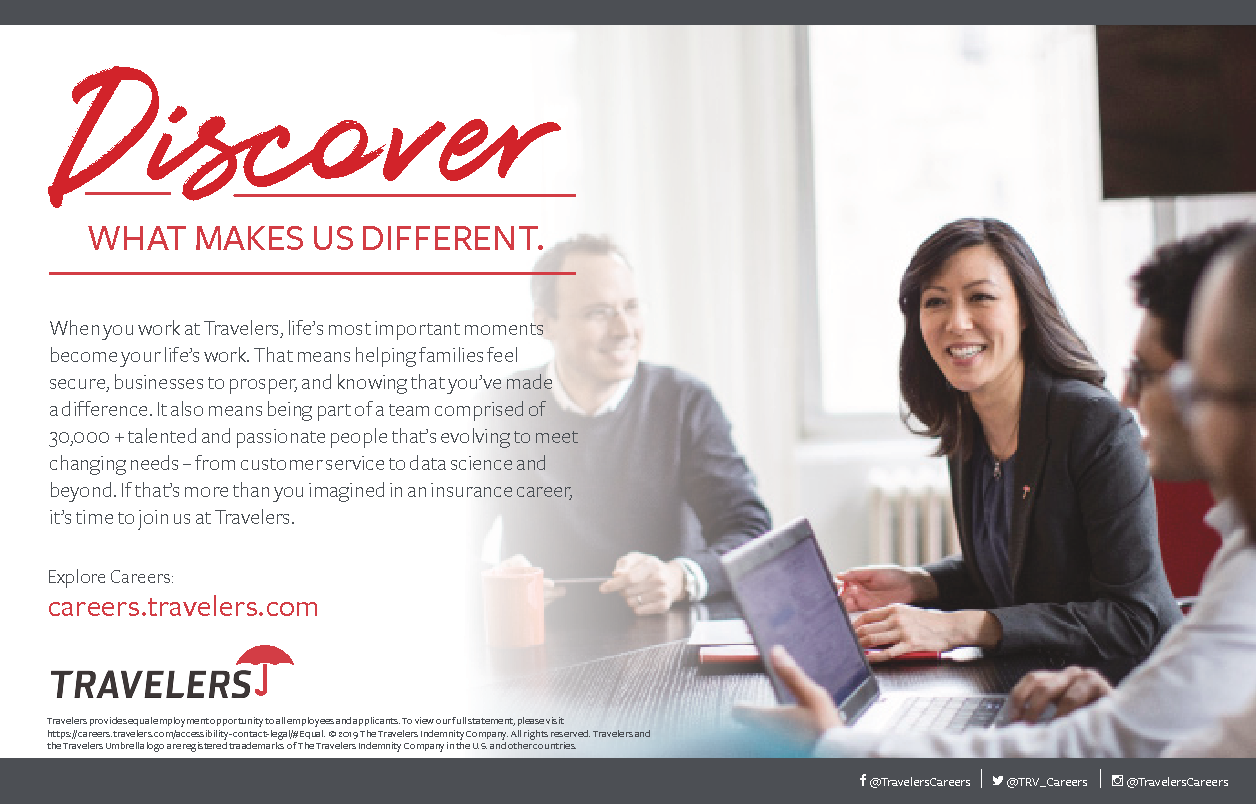
\includegraphics[width=\textwidth]{travelers.pdf}
\hfill

\includegraphics[width=\textwidth]{liberty.pdf}

\clearpage
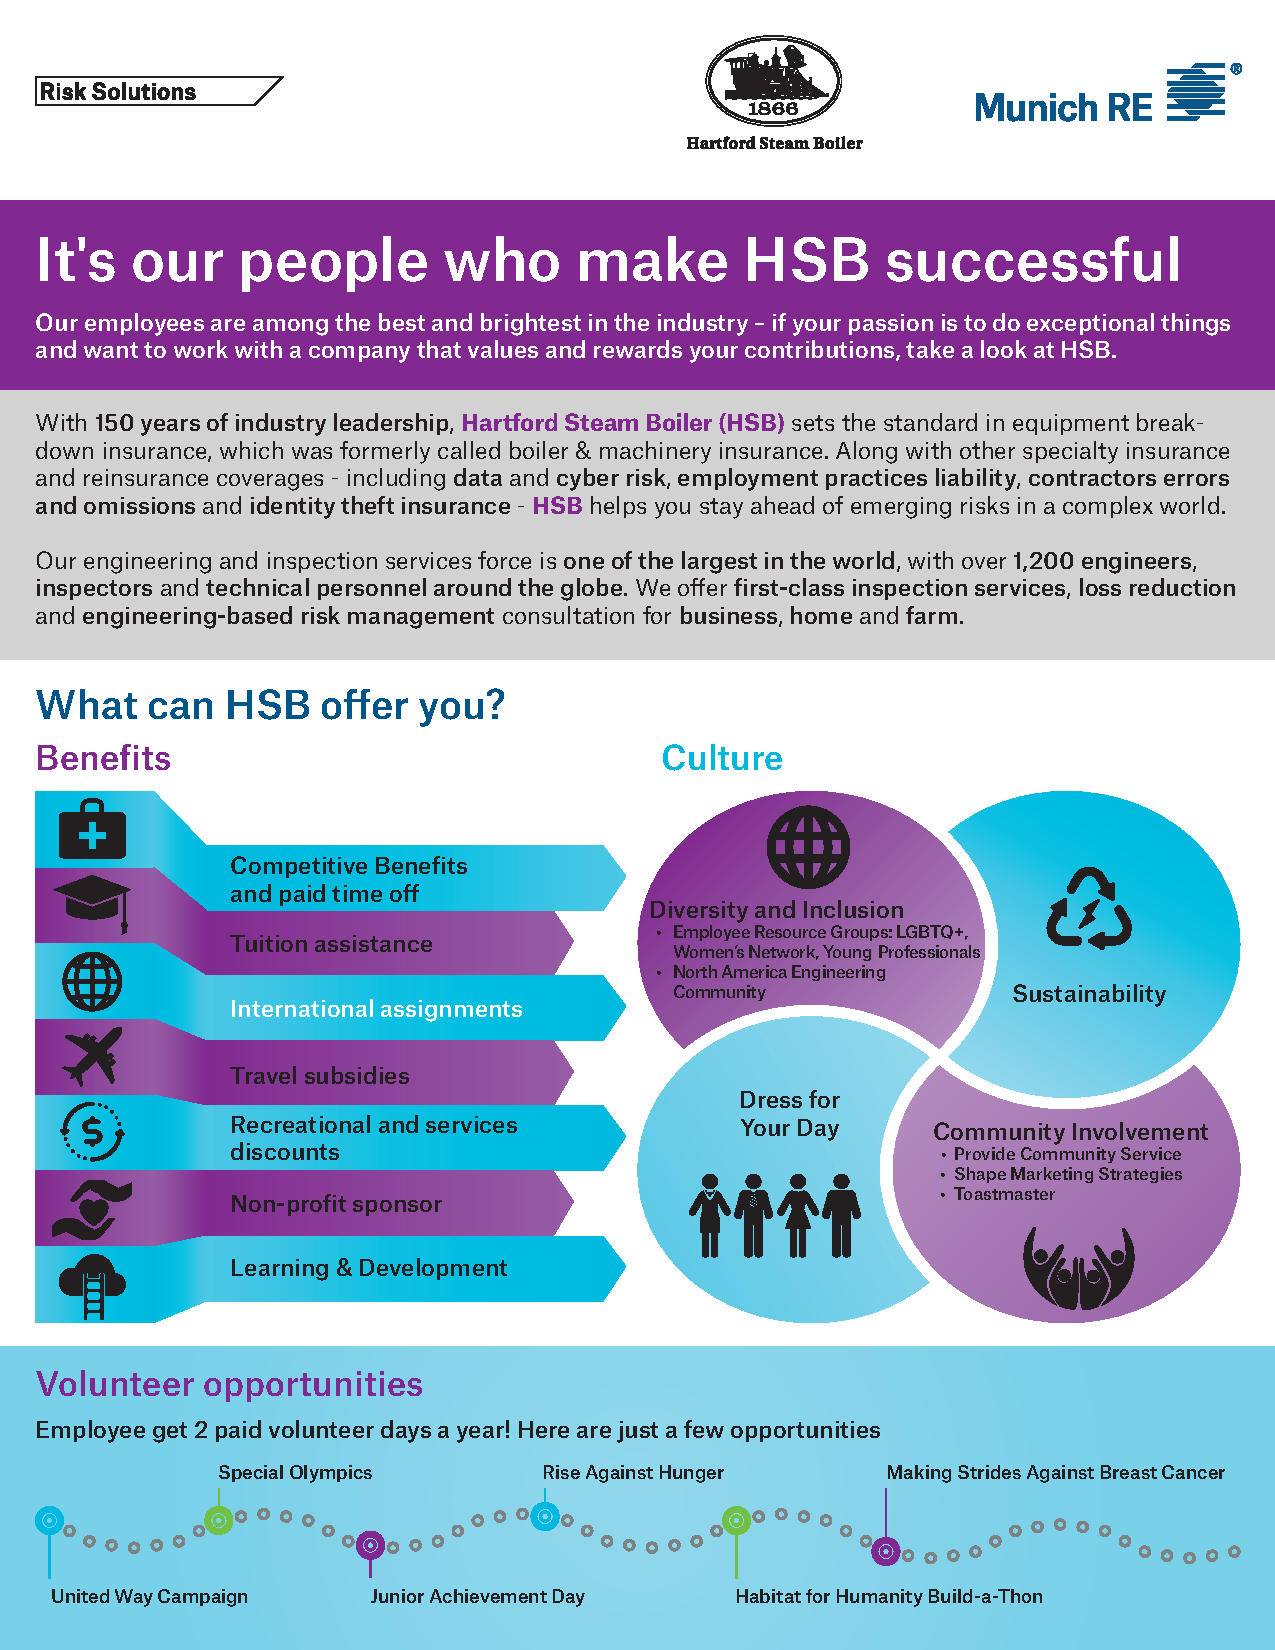
\includegraphics[page=1, width=\textwidth]{hsb.pdf}

\end{document}